\PassOptionsToPackage{unicode=true}{hyperref} % options for packages loaded elsewhere
\PassOptionsToPackage{hyphens}{url}
%
\documentclass[11pt,oneside]{report}
\usepackage{lmodern}
\usepackage{amssymb,amsmath}
\usepackage{ifxetex,ifluatex}
\usepackage{fixltx2e} % provides \textsubscript
\ifnum 0\ifxetex 1\fi\ifluatex 1\fi=0 % if pdftex
  \usepackage[T1]{fontenc}
  \usepackage[utf8]{inputenc}
  \usepackage{textcomp} % provides euro and other symbols
\else % if luatex or xelatex
  \usepackage{unicode-math}
  \defaultfontfeatures{Ligatures=TeX,Scale=MatchLowercase}
\fi
% use upquote if available, for straight quotes in verbatim environments
\IfFileExists{upquote.sty}{\usepackage{upquote}}{}
% use microtype if available
\IfFileExists{microtype.sty}{%
\usepackage[]{microtype}
\UseMicrotypeSet[protrusion]{basicmath} % disable protrusion for tt fonts
}{}
\IfFileExists{parskip.sty}{%
\usepackage{parskip}
}{% else
\setlength{\parindent}{0pt}
\setlength{\parskip}{6pt plus 2pt minus 1pt}
}
\usepackage{hyperref}
\hypersetup{
            pdftitle={R para Ciencia de Datos},
            pdfborder={0 0 0},
            breaklinks=true}
\urlstyle{same}  % don't use monospace font for urls
\usepackage[verbose,letterpaper,tmargin=25mm,bmargin=25mm,lmargin=20mm,rmargin=20mm]{geometry}
\usepackage{color}
\usepackage{fancyvrb}
\newcommand{\VerbBar}{|}
\newcommand{\VERB}{\Verb[commandchars=\\\{\}]}
\DefineVerbatimEnvironment{Highlighting}{Verbatim}{commandchars=\\\{\}}
% Add ',fontsize=\small' for more characters per line
\usepackage{framed}
\definecolor{shadecolor}{RGB}{248,248,248}
\newenvironment{Shaded}{\begin{snugshade}}{\end{snugshade}}
\newcommand{\AlertTok}[1]{\textcolor[rgb]{0.94,0.16,0.16}{#1}}
\newcommand{\AnnotationTok}[1]{\textcolor[rgb]{0.56,0.35,0.01}{\textbf{\textit{#1}}}}
\newcommand{\AttributeTok}[1]{\textcolor[rgb]{0.77,0.63,0.00}{#1}}
\newcommand{\BaseNTok}[1]{\textcolor[rgb]{0.00,0.00,0.81}{#1}}
\newcommand{\BuiltInTok}[1]{#1}
\newcommand{\CharTok}[1]{\textcolor[rgb]{0.31,0.60,0.02}{#1}}
\newcommand{\CommentTok}[1]{\textcolor[rgb]{0.56,0.35,0.01}{\textit{#1}}}
\newcommand{\CommentVarTok}[1]{\textcolor[rgb]{0.56,0.35,0.01}{\textbf{\textit{#1}}}}
\newcommand{\ConstantTok}[1]{\textcolor[rgb]{0.00,0.00,0.00}{#1}}
\newcommand{\ControlFlowTok}[1]{\textcolor[rgb]{0.13,0.29,0.53}{\textbf{#1}}}
\newcommand{\DataTypeTok}[1]{\textcolor[rgb]{0.13,0.29,0.53}{#1}}
\newcommand{\DecValTok}[1]{\textcolor[rgb]{0.00,0.00,0.81}{#1}}
\newcommand{\DocumentationTok}[1]{\textcolor[rgb]{0.56,0.35,0.01}{\textbf{\textit{#1}}}}
\newcommand{\ErrorTok}[1]{\textcolor[rgb]{0.64,0.00,0.00}{\textbf{#1}}}
\newcommand{\ExtensionTok}[1]{#1}
\newcommand{\FloatTok}[1]{\textcolor[rgb]{0.00,0.00,0.81}{#1}}
\newcommand{\FunctionTok}[1]{\textcolor[rgb]{0.00,0.00,0.00}{#1}}
\newcommand{\ImportTok}[1]{#1}
\newcommand{\InformationTok}[1]{\textcolor[rgb]{0.56,0.35,0.01}{\textbf{\textit{#1}}}}
\newcommand{\KeywordTok}[1]{\textcolor[rgb]{0.13,0.29,0.53}{\textbf{#1}}}
\newcommand{\NormalTok}[1]{#1}
\newcommand{\OperatorTok}[1]{\textcolor[rgb]{0.81,0.36,0.00}{\textbf{#1}}}
\newcommand{\OtherTok}[1]{\textcolor[rgb]{0.56,0.35,0.01}{#1}}
\newcommand{\PreprocessorTok}[1]{\textcolor[rgb]{0.56,0.35,0.01}{\textit{#1}}}
\newcommand{\RegionMarkerTok}[1]{#1}
\newcommand{\SpecialCharTok}[1]{\textcolor[rgb]{0.00,0.00,0.00}{#1}}
\newcommand{\SpecialStringTok}[1]{\textcolor[rgb]{0.31,0.60,0.02}{#1}}
\newcommand{\StringTok}[1]{\textcolor[rgb]{0.31,0.60,0.02}{#1}}
\newcommand{\VariableTok}[1]{\textcolor[rgb]{0.00,0.00,0.00}{#1}}
\newcommand{\VerbatimStringTok}[1]{\textcolor[rgb]{0.31,0.60,0.02}{#1}}
\newcommand{\WarningTok}[1]{\textcolor[rgb]{0.56,0.35,0.01}{\textbf{\textit{#1}}}}
\usepackage{graphicx,grffile}
\makeatletter
\def\maxwidth{\ifdim\Gin@nat@width>\linewidth\linewidth\else\Gin@nat@width\fi}
\def\maxheight{\ifdim\Gin@nat@height>\textheight\textheight\else\Gin@nat@height\fi}
\makeatother
% Scale images if necessary, so that they will not overflow the page
% margins by default, and it is still possible to overwrite the defaults
% using explicit options in \includegraphics[width, height, ...]{}
\setkeys{Gin}{width=\maxwidth,height=\maxheight,keepaspectratio}
\setlength{\emergencystretch}{3em}  % prevent overfull lines
\providecommand{\tightlist}{%
  \setlength{\itemsep}{0pt}\setlength{\parskip}{0pt}}
\setcounter{secnumdepth}{5}

% set default figure placement to htbp
\makeatletter
\def\fps@figure{htbp}
\makeatother

\AtBeginDocument{\let\maketitle\relax}

\usepackage{graphicx}
\usepackage{hyperref}
\hypersetup{colorlinks, citecolor=blue, filecolor=blue, linkcolor=blue, urlcolor=blue}
\usepackage{array}
\usepackage{color}
\definecolor{myblue}{RGB}{0, 24, 77}
\usepackage{afterpage}
\usepackage{tikz}
\usepackage{float}
%\usepackage{multicol}
%\usepackage{multirow}
%\usepackage{import}
%\graphicspath{{figuras/}}
\usepackage{enumerate}
\usepackage{fancyhdr}

\usepackage{titlesec}
\titleformat{\chapter}[display]
{\bfseries\large}
{\titlerule[1pt]%
\vspace{1pt}%
\titlerule
\vspace{1pc}%
\Large\MakeUppercase{\chaptertitlename} \thechapter}
{1pc}
{\titlerule
\vspace{1pc}%
\huge}
\titleformat{\section}
{\Large\bfseries}
{\thesection.}{.5em}{}
\titleformat{\subsection}
{\large \bfseries}
{\thesubsection.}{.5em}{}

\usepackage[spanish]{babel}
\usepackage[sfdefault,book]{FiraSans}
\usepackage{FiraMono}

\usepackage{tocloft}
\usepackage{wallpaper}

%para autoescalar imagenes
\makeatletter
\def\autoajuste{%
\ifdim\Gin@nat@width>\linewidth
\linewidth
\else
\Gin@nat@width
\fi
}
\makeatother

\setlength{\cftsecnumwidth}{3.5em}% Set length of number width in ToC for \section
\setlength{\cftsubsecnumwidth}{3.5em}% Make subsection numwidth the same as section
\setlength{\cftsubsecindent}{6em}% Make subsection indent the same as section

\makeatother

\parindent=0em
\parskip=1em

\title{R para Ciencia de Datos}
\author{}
\date{\vspace{-2.5em}}

\begin{document}
\maketitle

\pagenumbering{gobble}

\ThisLLCornerWallPaper{1}{portada.pdf}
\begin{center} \end{center}

\cleardoublepage

\newcommand{\HRule}{\rule{\linewidth}{0.5mm}}
\begin{titlepage}
{\sffamily 
    \begin{center}
        \vspace*{\fill}
        \rule{\linewidth}{0.5mm}\\[0.4cm]{
        \huge \bfseries R PARA CIENCIA DE DATOS}\\ [0.4cm]
        \rule{\linewidth}{0.5mm}\\[1.5cm]
        %Authors
        \begin{minipage}{0.9\textwidth}
        \begin{center}
        \large
        HADLEY WICKHAM \& GARETT GROLEMUND
        \end{center}
        \end{minipage}
    \vfill
    \end{center}}
\end{titlepage}
\setcounter{page}{2}

\setlength\parindent{0pt}

\renewcommand{\labelenumi}{\alph{enumi}.}

\newpage

\chapter*{R Para Ciencia de Datos}

HADLEY WICKHAM \& GARETT GROLEMUND

Este libro se distribuye de forma gratuita en
\href{https://github.com/cienciadedatos/datos}{https://github.com/cienciadedatos/datos}

La presente versión fue compilada el día 14 de junio de 2020.

\copyright 2016, 2017, 2018 Hadley Wickham \& Garett Grolemund

\vfill

\begin{center}

\includegraphics[width=5cm]{by-nc-nd.pdf}
\end{center}

Esta obra se distribuye bajo los términos y condiciones de la licencia
\href{http://creativecommons.org/licenses/by-nc-nd/3.0/us/}{Creative
Commons Atribución-No Comercial-Sin Derivados 3.0} vigente en los
Estados Unidos de América.

\newpage
\tableofcontents
\newpage

\pagenumbering{arabic}
\setcounter{page}{1}

\chapter*{Bienvenida}

Este es el sitio web de la versión en español de \textbf{``R for Data
Science''}, de Hadley Wickham y Garrett Grolemund. Este texto te
enseñará cómo hacer ciencia de datos con R: aprenderás a importar datos,
llevarlos a la estructura más conveniente, transformarlos, visualizarlos
y modelarlos. Así podrás poner en pŕactica las habilidades necesarias
para hacer ciencia de datos. Tal como los químicos aprenden a limpiar
tubos de ensayo y ordenar un laboratorio, aprenderás a limpiar datos y
crear gráficos--- junto a muchas otras habilidades que permiten que la
ciencia de datos tenga lugar. En este libro encontrarás las mejores
prácticas para desarrollar dichas tareas usando R. También aprenderás a
usar la gramática de gráficos, programación letrada e investigación
reproducible para ahorrar tiempo. Además, aprenderás a manejar recursos
cognitivos para facilitar el hacer descubrimientos al momento de
manipular, visualizar y explorar datos.

\section*{Sobre la traducción}

La traducción de ``R para Ciencia de Datos'' es un proyecto colaborativo
de la comunidad de R de Latinoamérica, que tiene por objetivo hacer R
más accesible en la región. .

En la traducción del libro participaron las siguientes personas (en
orden alfabético): Marcela Alfaro, Mónica Alonso, Fernando Álvarez,
Zulemma Bazurto, Yanina Bellini, Juliana Benítez, María Paula Caldas,
Elio Campitelli, Florencia D'Andrea, Rocío Espada, Joshua Kunst,
Patricia Loto, Pamela Matías, Lina Moreno, Paola Prieto, Riva Quiroga,
Lucía Rodríguez, Mauricio ``Pachá'' Vargas, Daniela Vázquez, Melina
Vidoni, Roxana N. Villafañe. ¡Muchas gracias por su trabajo! La
administración del repositorio con la traducción ha estado cargo de
Mauricio ``Pachá'' Vargas. La coordinación general y la edición, a cargo
de Riva Quiroga.

Agradecemos a todas las personas que han ayudado revisando las
traducciones y haciendo sugerencias de mejora. Puedes revisar la
\href{https://github.com/cienciadedatos/documentacion-traduccion-r4ds/blob/master/creditos-participacion.md}{documentación
del proyecto} para ver los créditos de participación. Gracias también a
Marcela Alfaro por
\href{https://twitter.com/Fichulina/status/943509009318981633}{el tuit}
que hizo visible la necesidad de la versión en español, y a Laura Ación
y Edgar Ruiz, que pusieron en contacto a las personas del equipo.

Este proyecto no solo implica la traducción del texto, sino también de
los sets de datos que se utilizan a lo largo de él. Para ello, se creó
el paquete \texttt{datos}, que contiene las versiones traducidas de
estos. Puedes revisar su documentación
\href{https://cienciadedatos.github.io/datos}{acá}. El paquete fue
desarrollado por Edgar Ruiz, Riva Quiroga, Mauricio ``Pachá'' Vargas y
Mauro Lepore. Para su creación se utilizaron funciones del paquete
\texttt{datalang} de Edgar Ruiz y las sabias sugerencias de Hadley
Wickham.\\
Si quieres conocer más sobre los principios que han orientado nuestro
trabajo puedes leer {[}la documentación del proyecto{]}
(https://github.com/cienciadedatos/documentacion-traduccion-r4ds). Para
estar al tanto de novedades sobre el paquete \{datos\} y nuevas
iniciativas del equipo, \href{https://twitter.com/R4DS_es}{sigue nuestra
cuenta en Twitter}.

\section*{Sobre la versión original en inglés}

Puedes consultar la versión original del libro en
\href{http://r4ds.had.co.nz/}{r4ds.had.co.nz/}. Existe una edición
impresa, que fue publicada por O'Reilly en enero de 2017. Puedes
adquirir una copia en \href{http://amzn.to/2aHLAQ1}{Amazon}.

(El libro ``R for Data Science'' primero se llamó ``Data Science with
R'' en ``Hands-On Programming with R'')

Esta obra se distribuye bajo los términos y condiciones de la licencia
\href{http://creativecommons.org/licenses/by-nc-nd/3.0/us/}{Creative
Commons Atribución-No Comercial-Sin Derivados 3.0} vigente en los
Estados Unidos de América.

\hypertarget{introducciuxf3n}{%
\chapter{Introducción}\label{introducciuxf3n}}

La ciencia de datos (\emph{data science}) es una disciplina fascinante
que te permite convertir datos sin procesar en entendimiento,
comprensión y conocimiento. El objetivo de este libro es ayudarte a
aprender las herramientas más importantes para que puedas hacer ciencia
de datos en R. Luego de leerlo, tendrás las herramientas para enfrentar
una gran variedad de desafíos propios de esta área, usando las mejores
partes de R.

\hypertarget{lo-que-aprenderuxe1s}{%
\section{Lo que aprenderás}\label{lo-que-aprenderuxe1s}}

La ciencia de datos es un campo muy amplio y no hay manera de que puedas
dominarlo leyendo un solo libro. El objetivo de este, en particular, es
entregarte una base sólida acerca de las herramientas más importantes.
Nuestro modelo sobre cuáles son las herramientas necesarias para un
proyecto típico de ciencia de datos se ve así:

\begin{center}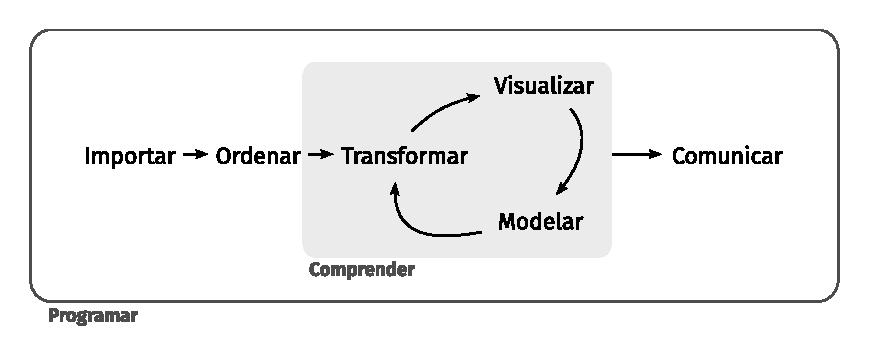
\includegraphics[width=0.75\linewidth]{diagrams_pdf/es/data-science} \end{center}

Primero, debes \textbf{importar} tus datos hacia R. Típicamente, esto
implica tomar datos que están guardados en un archivo, base de datos o
API y cargarlos como \emph{data frame} en R. Si no puedes llevar tus
datos a R, no puedes hacer ciencia de datos con él.

Una vez que has importado los datos, es una buena idea
\textbf{ordenarlos}. Ordenar los datos significa guardarlos de una
manera consistente que haga coincidir la semántica del set de datos con
la manera en que está guardado. En definitiva, cuando tus datos están
ordenados, cada columna es una variable y cada fila una observación.
Tener datos ordenados es importante porque si su estructura es
consistente, puedes enfocar tus esfuerzos en las preguntas sobre los
datos y no en luchar para que estos tengan la forma necesaria para
diferentes funciones.

Cuando tus datos están ordenados, un primer paso suele ser
\textbf{transformarlos}. La transformación implica reducir las
observaciones a aquellas que sean de interés (como todas las personas de
una ciudad o todos los datos del último año), crear nuevas variables que
sean funciones de variables ya existentes (como calcular la rapidez a
partir de la velocidad y el tiempo) y calcular una serie de estadísticos
de resumen (como recuentos y medias). Juntos, a ordenar y transformar,
se les llama \textbf{manejar o domar} los datos, porque hacer que estos
tengan la forma con la que es natural trabajarlos, suele sentirse como
una lucha.

Una vez que tienes los datos ordenados con las variables que necesitas,
hay dos principales fuentes generadoras de conocimiento: la
visualización y el modelado. Ambas tienen fortalezas y debilidades
complementarias, por lo que cualquier análisis real iterará entre ellas
varias veces.

La \textbf{visualización} es una actividad humana fundamental. Una buena
visualización te mostrará cosas que no esperabas o hará surgir nuevas
preguntas acerca de los datos. También puede darte pistas acerca de si
estás haciendo las preguntas equivocadas o si necesitas recolectar datos
diferentes. Las visualizaciones pueden sorprenderte, pero no escalan
particularmente bien, ya que requieren ser interpretadas por una
persona.

Los \textbf{modelos} son herramientas complementarias a la
visualización. Una vez que tus preguntas son lo suficientemente
precisas, puedes utilizar un modelo para responderlas. Los modelos son
herramientas matemáticas o computacionales, por lo que generalmente
escalan bien. Incluso cuando no lo hacen, resulta más económico comprar
más computadores que comprar más cerebros. Sin embargo, cada modelo
tiene supuestos y, debido a su propia naturaleza, un modelo no puede
cuestionar sus propios supuestos. Esto significa que un modelo, por
definición, no puede sorprenderte.

El último paso de la ciencia de datos es la \textbf{comunicación}, una
parte crítica de cualquier proyecto de análisis de datos. No importa qué
tan bien tus modelos y visualizaciones te hayan permitido entender tus
datos, a menos que también puedas comunicar esos resultados a otras
personas.

Alrededor de todas estas herramientas se encuentra la
\textbf{programación}. La programación es una herramienta transversal
que usarás en todas las partes de tu proyecto. No necesitas ser una
personas experta en programación para hacer ciencia de datos, pero
aprender más sobre ella es una gran ventaja porque te permite
automatizar tareas recurrentes y resolver problemas con mayor facilidad.

En cualquier proyecto de ciencia de datos tendrás que ocupar estas
herramientas, pero en muchos casos estas no serán suficientes. Hay un
regla aproximada de 80-20 en juego: puedes enfrentar alrededor del 80 \%
de cualquier proyecto usando las herramientas que aprenderás en este
libro, pero necesitarás utilizar otras para abordar el 20 \% restante. A
lo largo del libro te iremos señalando recursos donde puedes aprender
más.

\hypertarget{cuxf3mo-estuxe1-organizado-este-libro}{%
\section{Cómo está organizado este
libro}\label{cuxf3mo-estuxe1-organizado-este-libro}}

La descripción anterior de las herramientas propias de las ciencia de
datos está organizada aproximadamente de acuerdo al orden en que
usualmente se usan en el análisis (aunque, por supuesto, tendrás que
iterar entre ellas múltiples veces). Sin embargo, en nuestra experiencia
esa no es la mejor manera de aprenderlas:

\begin{itemize}
\item
  Partir con la ingesta y orden de los datos no es lo óptimo porque el
  80\% del tiempo es un proceso rutinario y aburrido y el 20\% restante
  es extraño y frustrante. ¡No es un buen lugar para aprender un tema
  nuevo! En cambio, partiremos con la visualización y transformación de
  datos que ya han sido importados y ordenados. De esta manera, cuando
  tengas que importar y ordenar tus propios datos, tu motivación se
  mantendrá alta porque sabrás que ese sufrimiento vale la pena.
\item
  Algunos temas se explican mejor con otras herramientas. Por ejemplo,
  creemos que es más fácil entender qué es un modelo si ya sabes sobre
  visualización, datos ordenados y programación.
\item
  Las herramientas de programación no son necesariamente interesantes en
  sí mismas; sin embargo, te permiten enfrentar problemas desafiantes.
  Te entregaremos una selección de herramientas de programación en la
  mitad del libro y luego verás cómo se pueden combinar con las
  herramientas propias de la ciencia de datos para enfrentar problemas
  de modelado interesantes.
\end{itemize}

En cada capítulo hemos tratado de mantener un patrón similar: partir con
algunos ejemplos motivantes que te permitan ver el panorama completo y
luego sumergirnos en los detalles. Cada sección del libro incluye
ejercicios que te ayudarán a practicar lo que has aprendido. Pese a que
puede ser tentador saltarse los ejercicios, no hay mejor manera de
aprender que practicar con problemas reales.

\hypertarget{quuxe9-no-vas-a-aprender}{%
\section{Qué no vas a aprender}\label{quuxe9-no-vas-a-aprender}}

Hay algunos temas importantes que este libro no aborda. Creemos que es
importante mantenernos enfocados con determinación en los aspectos
esenciales, con el fin de que puedas ponerte en marcha lo más rápido
posible. Eso implica que este libro no puede abordar todos los temas
importantes.

\hypertarget{big-data}{%
\subsection{Big data}\label{big-data}}

Este libro se enfoca con orgullo en conjuntos de datos pequeños
procesables en la memoria de tu computadora. Este es el lugar adecuado
para partir, ya que no es posible que te enfrentes a datos de gran
tamaño sin antes haber tenido experiencia con otros más pequeños. Las
herramientas que aprenderás en este libro permiten manejar fácilmente
datos de cientos de megabytes y, con un poco de cuidado, normalmente
podrías hacerlas funcionar con 1 o 2 Gb de datos. Si habitualmente
trabajas con datos más grandes (por ejemplo, 10-100 Gb), sería bueno que
aprendieras sobre
\href{https://github.com/Rdatatable/data.table}{data.table}. Este libro
no enseña \texttt{data.table}, ya que su interfaz concisa hace que sea
difícil de aprender por las pocas pistas lingüísticas que entrega. Sin
embargo, si trabajas con datos grandes, la ventaja en términos de
rendimiento hace que valga la pena el esfuerzo extra que requiere
aprenderlo. Si tus datos son más grandes que eso, es importante que
consideres cuidadosamente si tu problema de \emph{big data} no es, en
realidad, un problema de datos pequeños oculto. Si bien los datos
completos pueden ser grandes, muchas veces los necesarios para responder
una pregunta específica son menos. Puede que encuentres un subconjunto,
una submuestra o un resumen de datos que sí caben en la memoria y que de
todos modos te permiten responder la pregunta que te interesa. El
desafío en este caso es encontrar los datos pequeños adecuados, lo que
usualmente requiere muchas iteraciones.

Otra posibilidad es que tu problema de \emph{big data} sea realmente una
suma de problemas de datos pequeños. Puede que cada uno de estos
problema individuales quepa en la memoria; el problema es que tienes
millones de ellos. Por ejemplo, puedes querer ajustar un modelo para
cada persona de tu conjunto de datos. Eso sería trivial si tuvieras solo
10 o 100 personas, pero no si tienes un millón. Afortunadamente, cada
problema es independiente del resto (una configuración a la que a veces
se le llama de manera vergonzosa \emph{paralela}), por lo que solo
necesitas un sistema (como Hadoop o Spark) que te permita enviar
diferentes sets de datos a diferentes computadoras para procesarlos. Una
vez que hayas resuelto cómo responder la pregunta para un subset de
datos usando las herramientas descritas en este libro, podrás aprender
otras nuevas como \texttt{sparklyr}, \texttt{RHIPE} y \texttt{ddr} para
responder la pregunta para todo el \emph{dataset}.

\hypertarget{python-julia-y-amigos}{%
\subsection{Python, Julia y amigos}\label{python-julia-y-amigos}}

En este libro no aprenderás nada sobre Python, Julia u otros lenguajes
de programación útiles para hacer ciencia de datos. No es que creamos
que estas herramientas sean malas. ¡No lo son! En la práctica, la
mayoría de los equipos de ciencia de datos utilizan una mezcla de
lenguajes, habitualmente al menos R y Python.

Sin embargo, creemos fuertemente que es preferible dominar una sola
herramienta a la vez. Mejorarás más rápido si te sumerges en un tema con
profundidad, en vez de dispersarte entre muchos temas distintos. Esto no
quiere decir que solo tengas que saber una cosa, solamente que
aprenderás más rápido si te enfocas en una a la vez. Debes tratar de
aprender cosas nuevas a lo largo de tu carrera, pero asegúrate de que tu
entendimiento sea sólido antes de moverte hacia el siguiente tema
interesante.

Creemos que R es un gran lugar para empezar tu camino en la ciencia de
datos, ya que es un ambiente diseñado desde las bases hacia arriba para
apoyarla. R no es solo un lenguaje de programación, sino también un
ambiente interactivo para hacer ciencia de datos. Para apoyar esta
interacción, R es mucho más flexible que muchos de sus equivalentes. Si
bien esta flexibilidad tiene desventajas, su lado positivo es que
permite desarrollar con facilidad gramáticas que se ajustan a las
distintas partes de la ciencia de datos. Estos mini-lenguajes te ayudan
a pensar los problemas como científico/a de datos, al tiempo que apoyan
una interacción fluida entre tu cerebro y la computadora.

\hypertarget{datos-no-rectangulares}{%
\subsection{Datos no rectangulares}\label{datos-no-rectangulares}}

Este libro se enfoca exclusivamente en datos rectangulares, esto es, en
conjuntos de valores que están asociados cada uno con una variable y una
observación. Hay muchos conjuntos de datos que no se ajustan
naturalmente a este paradigma, los que incluyen imágenes, sonidos,
árboles y texto. Sin embargo, los \emph{data frames} rectangulares son
tan comunes en la ciencia y en la industria, que creemos que son un buen
lugar para iniciar tu camino en la ciencia de datos.

\hypertarget{confirmaciuxf3n-de-hipuxf3tesis}{%
\subsection{Confirmación de
hipótesis}\label{confirmaciuxf3n-de-hipuxf3tesis}}

Es posible dividir el análisis de datos en dos áreas: generación de
hipótesis y confirmación de hipótesis (a veces llamada análisis
confirmatorio). El foco de este libro está puesto decididamente en la
generación de hipótesis o exploración de datos. Acá mirarás con
profundidad los datos y, en combinación con tu propio conocimiento,
generarás muchas hipótesis interesantes que ayudarán a explicar por qué
se comportan como lo hacen. Evaluarás las hipótesis informalmente,
usando tu escepticismo para cuestionar los datos de distintas maneras.

El complemento de la generación de hipótesis es la confirmación de
hipótesis. Esta última es difícil por dos razones:

\begin{enumerate}
\def\labelenumi{\arabic{enumi}.}
\item
  Necesitas un modelo matemático con el fin de generar predicciones
  falseables. Esto usualmente requiere considerable sofisticación
  estadística.
\item
  Cada observación puede ser utilizada una sola vez para confirmar una
  hipótesis. En el momento en que la usas más de una vez ya estás de
  vuelta haciendo análisis exploratorio. Esto quiere decir que para
  hacer confirmación de hipótesis tienes que haber ``pre-registrado''
  (es decir, haber escrito con anticipación) tu plan de análisis y no
  desviarte de él incluso cuando hayas visto tus datos. Hablaremos un
  poco acerca de estrategias que puedes utilizar para hacer esto más
  fácil en el capítulo sobre \protect\hyperlink{model-intro}{modelos}.
\end{enumerate}

Es habitual pensar en el modelado como una herramienta para la
confirmación de hipótesis y a la visualización como una herramienta para
la generación de hipótesis. Sin embargo, esa es una falsa dicotomía: los
modelos son utilizados usualmente para la exploración y, con un poco de
cuidado, puedes usar la visualización para confirmar una hipótesis. La
diferencia clave es qué tan seguido mires cada observación: si la miras
solo una vez es confirmación; si la miras más de una vez es exploración.

\hypertarget{prerrequisitos}{%
\section{Prerrequisitos}\label{prerrequisitos}}

Hemos asumido algunas cosas respecto de lo que ya sabes con el fin de
poder sacar mayor provecho de este libro. Tienes que tener una
\emph{literacidad} numérica general y sería útil que tuvieses algo de
experiencia programando. Si nunca has programado antes y puedes leer en
inglés, \href{https://rstudio-education.github.io/hopr/}{Hands on
Programming with R} escrito por Garrett podría ser un buen
acompañamiento para este libro.

Hay cinco cosas que necesitas para poder ejecutar el código incluido en
este libro: R, RStudio, una colección de paquetes llamada
\textbf{tidyverse}, el paquete \textbf{datos} (que incluye los datos en
español se se utilizan en los ejemplos y ejercicios) y una serie de
otros paquetes. Los paquetes son la unidad fundamental de código
reproducible de R. Incluyen funciones reutilizables, la documentación
que describe cómo usarlas y datos de muestra.

\hypertarget{r}{%
\subsection{R}\label{r}}

Para descargar R debes acceder a CRAN, llamado así por sus siglas en
inglés: the \textbf{c}omprehensive \textbf{R} \textbf{a}rchive
\textbf{n}etwork. CRAN está compuesto de una serie de servidores espejo
repartidos alrededor del mundo y es utilizado para distribuir tanto R
como los paquetes de R. No es necesario que intentes elegir un servidor
que esté cerca tuyo: en su lugar, puedes utilizar el servidor en la
nube, \url{https://cloud.r-project.org}, que automáticamente lo
identifica por ti.

Una vez al año sale una nueva versión importante de R y hay entre 2 y 3
ediciones menores en ese período. Es una buena idea actualizarlo
regularmente. El proceso puede ser un poco engorroso, especialmente en
el caso de las versiones mayores, que requieren que reinstales todos los
paquetes que ya tienes. Sin embargo, no hacerlo puede ser peor. Para
este libro, asegúrate de tener al menos la versión 3.5.

\hypertarget{rstudio}{%
\subsection{RStudio}\label{rstudio}}

RStudio es un ambiente de desarrollo integrado (o IDE, por su sigla en
inglés: Integrated Development Environment) para programar en R. Puedes
descargarlo e instalarlo desde \url{http://www.rstudio.com/download}.
RStudio se actualiza un par de veces al año. Cuando haya una nueva
versión disponible, el mismo programa te lo hará saber. Es una buena
idea mantenerlo actualizado para que puedas aprovechar las mejores y más
recientes características. Para este libro, asegúrate de tener al menos
la versión 1.0.0.

Cuando abras RStudio, verás en la interfaz dos regiones clave:

\begin{center}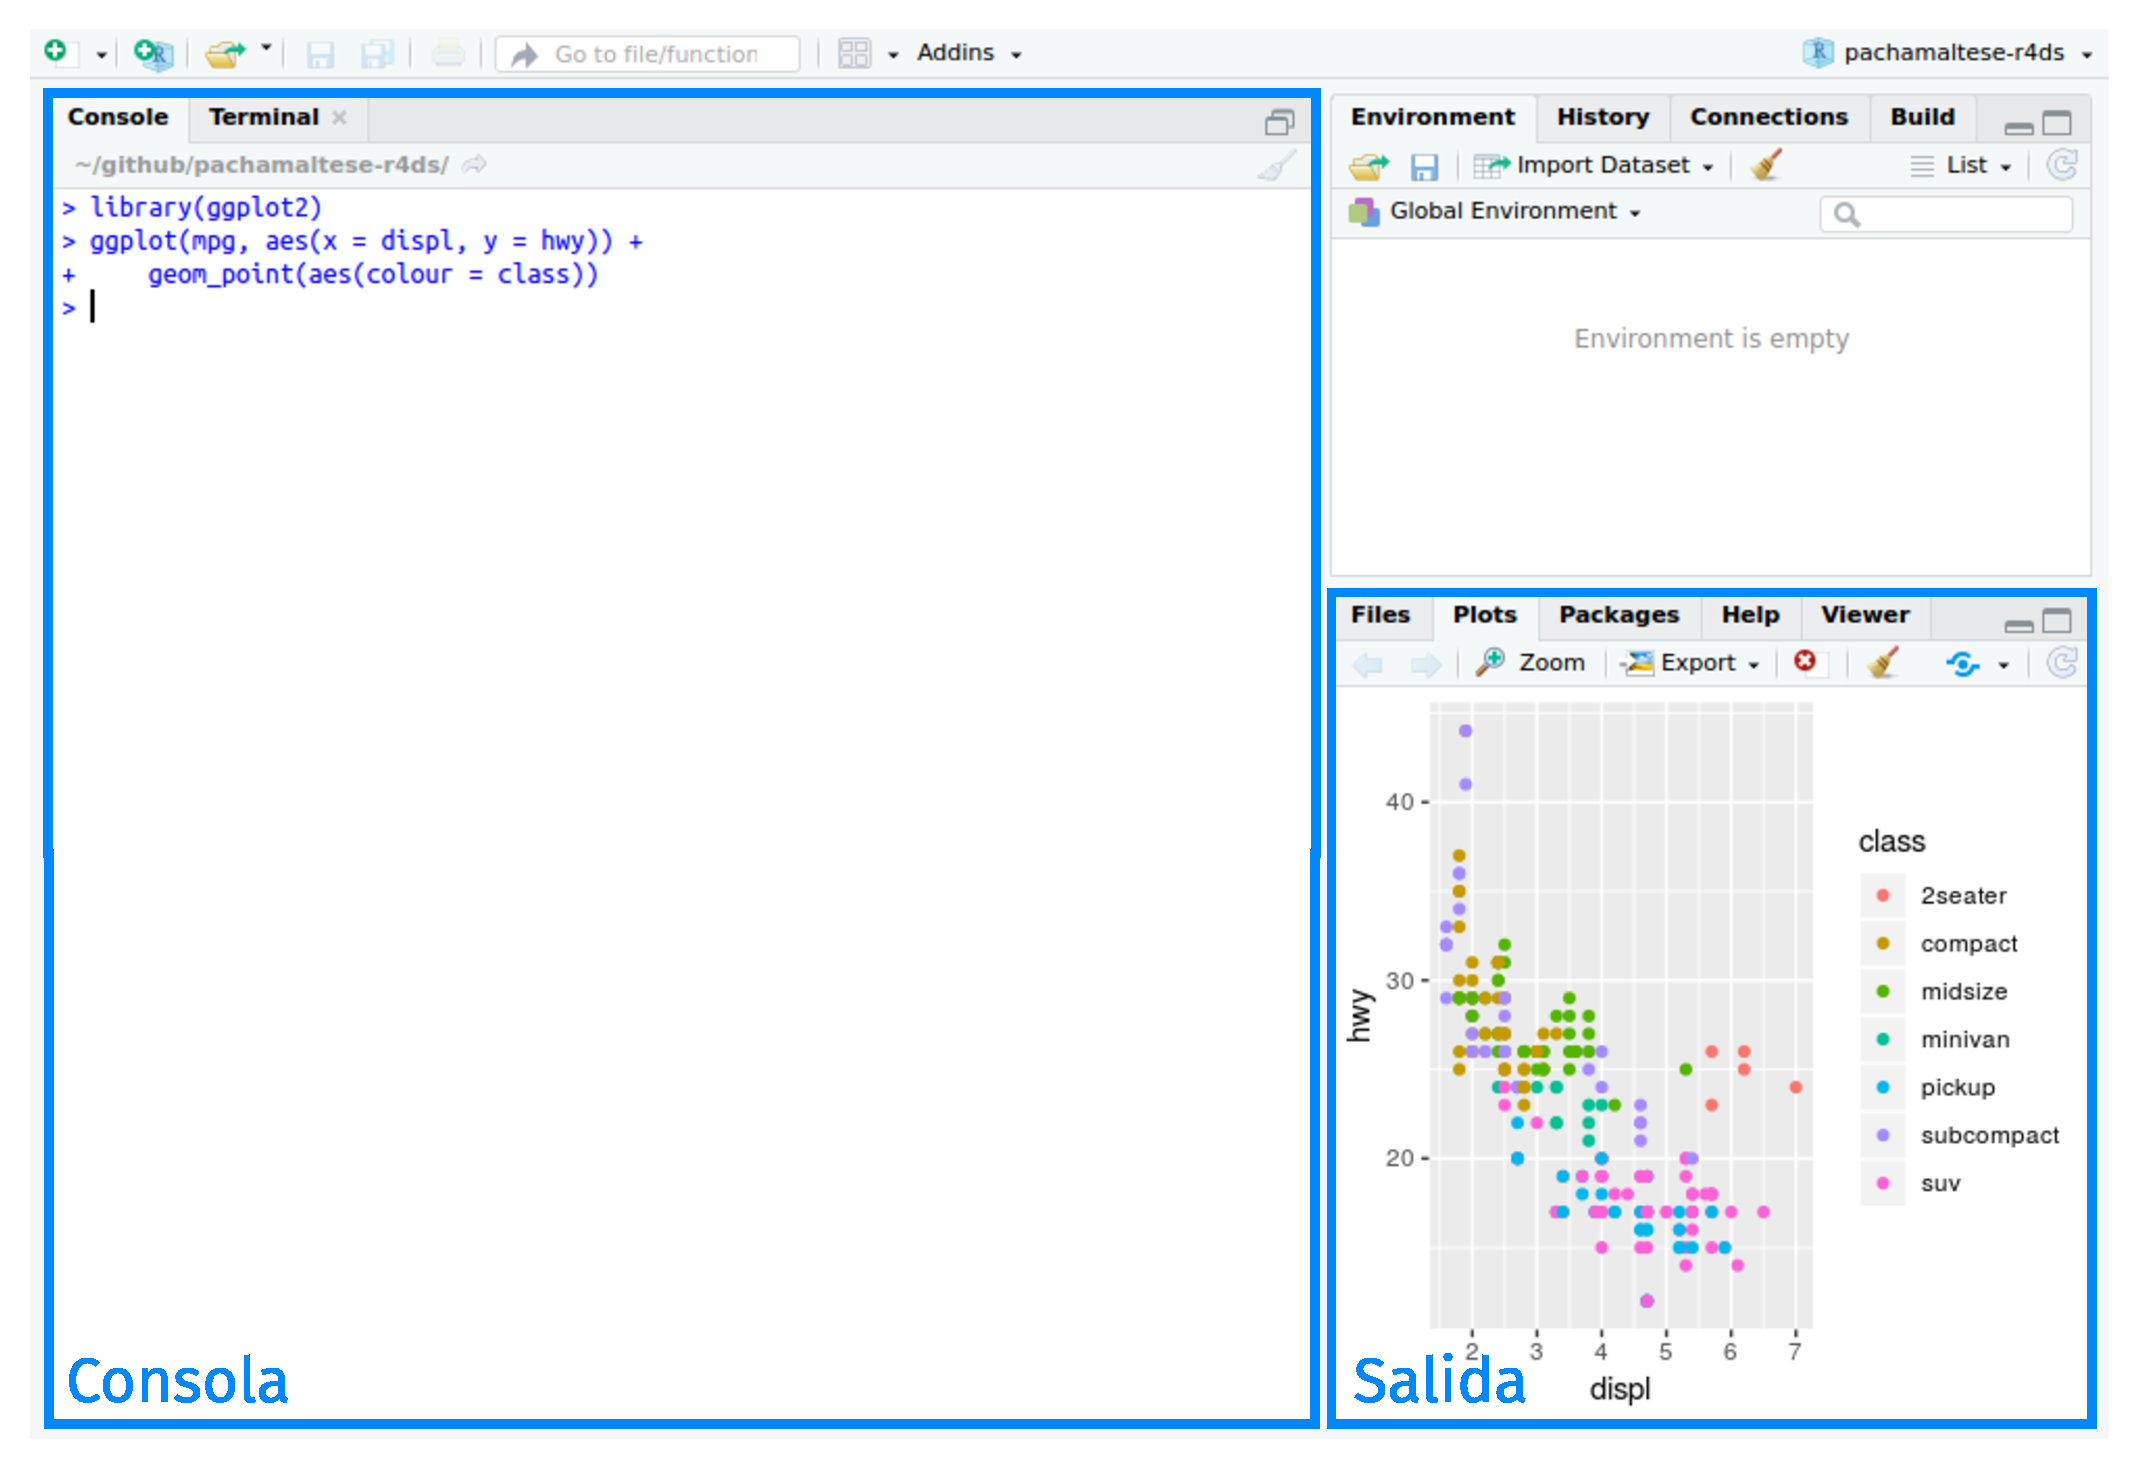
\includegraphics[width=0.75\linewidth]{diagrams_pdf/es/rstudio-console} \end{center}

Por ahora, todo lo que tienes que saber es que el código de R se escribe
en la Consola y que hay que presionar Enter para ejecutarlo. ¡Aprenderás
más a medida que avancemos!

\hypertarget{el-tidyverse}{%
\subsection{El Tidyverse}\label{el-tidyverse}}

Es necesario que instales también algunos paquetes de R. Un
\textbf{paquete} es una colección de funciones, datos y documentación
que permite extender las capacidades de R base. Los paquetes son clave
para usar R de manera exitosa. La mayoría de los paquetes que aprenderás
a usar en este libro son parte del llamado ``Tidyverse''. Los paquetes
del Tidyverse comparten una filosofía acerca de los datos y la
programación en R, y están diseñados para trabajar juntos con
naturalidad. Su nombre viene de la palabra en inglés ``tidy'', que
quiere decir ``ordenado''.

Puedes instalar el \textbf{tidyverse} completo con una sola línea de
código:

\begin{Shaded}
\begin{Highlighting}[]
\KeywordTok{install.packages}\NormalTok{(}\StringTok{"tidyverse"}\NormalTok{)}
\end{Highlighting}
\end{Shaded}

Escribe en tu computadora esa línea de código en la consola y luego
presiona Enter para ejecutarla. R descargará los paquetes de CRAN y los
instalará en tu computadora. Si tienes problemas durante la instalación,
asegúrate que tienes conexión a Internet y que
\url{https://cloud.r-project.org/} no está bloqueado por tu firewall o
proxy.

No podrás usar las funciones, objetos y archivos de ayuda de un paquete
hasta que lo hayas cargado con \texttt{library()}. Una vez que has
instalado un paquete, puedes cargarlo con la función \texttt{library()}:

\begin{Shaded}
\begin{Highlighting}[]
\KeywordTok{library}\NormalTok{(tidyverse)}
\end{Highlighting}
\end{Shaded}

Este mensaje te indica que el tidyverse está cargando los paquetes
\textbf{ggplot2}, \textbf{tibble}, \textbf{tidyr}, \textbf{readr},
\textbf{purrr}, \textbf{dplyr}, \textbf{stringr} y \textbf{forcats}.
Estos son considerados el \textbf{corazón} del Tidyverse porque los
usarás prácticamente en cualquier análisis.

Los paquetes del Tidyverse cambian con bastante frecuencia. Puedes ver
si existen actualizaciones disponibles y opcionalmente instalarlas
ejecutando \texttt{tidyverse\_update()}.

\hypertarget{el-paquete-datos}{%
\subsection{\texorpdfstring{El paquete
\texttt{datos}}{El paquete datos}}\label{el-paquete-datos}}

Con el fin de que este libro sea más accesible para el público
hispanoparlante, además de la traducción del texto se han traducido los
datos que se utilizan en los ejemplos y ejercicios.

El paquete \texttt{datos} se encuentra disponible en Github y puedes
instalarlo ejecutando el siguiente código:

\begin{Shaded}
\begin{Highlighting}[]
\CommentTok{#install.packages("remotes")}
\NormalTok{remotes}\OperatorTok{::}\KeywordTok{install_github}\NormalTok{(}\StringTok{"cienciadedatos/datos"}\NormalTok{)}
\end{Highlighting}
\end{Shaded}

\hypertarget{otros-paquetes}{%
\subsection{Otros paquetes}\label{otros-paquetes}}

Existen muchas otros paquetes excelentes que no son parte del
\textbf{tidyverse} porque resuelven problemas de otros ámbitos o porque
los principios en los que se basa su diseño son distintos. Esto no los
hace mejores o peores, solo diferentes. En otras palabras, el
complemento del \textbf{tidyverse} no es el \emph{messyverse} (del
inglés \emph{messy}, desordenado), sino muchos otros universos de
paquetes interrelacionados. A medida que te enfrentes a más proyectos de
ciencia de datos con R, aprenderás sobre nuevos paquetes y nuevas formas
de pensar los datos.

\hypertarget{ejecutar-cuxf3digo-en-r}{%
\section{Ejecutar código en R}\label{ejecutar-cuxf3digo-en-r}}

En la sección anterior te mostramos algunos ejemplos de cómo ejecutar
código en R. En el libro, el código se ve así:

\begin{Shaded}
\begin{Highlighting}[]
\DecValTok{1} \OperatorTok{+}\StringTok{ }\DecValTok{2}
\end{Highlighting}
\end{Shaded}

\begin{verbatim}
[1] 3
\end{verbatim}

\begin{Shaded}
\begin{Highlighting}[]
\CommentTok{#> [1] 3}
\end{Highlighting}
\end{Shaded}

Si ejecutas el mismo código en tu consola local, se verá así:

\begin{verbatim}
> 1 + 2
[1] 3
\end{verbatim}

Hay dos diferencias principales. La primera, es que en tu consola debes
escribir el código después del signo \texttt{\textgreater{}}, llamado
\emph{prompt}; en el libro no te mostraremos el \emph{prompt}. La
segunda, es que en el libro el \emph{output}, es decir, el resultado de
ejecutar el código, está comentado: \texttt{\#\textgreater{}}. En tu
consola, el output aparecerá directamente después del código. Estas dos
diferencias implican que, como esta es una versión electrónica del
libro, puedes copiar directamente el código que aparece acá y pegarlo en
tu consola.

A lo largo del libro usaremos una serie consistente de convenciones para
referirnos al código:

\begin{itemize}
\item
  Las funciones están escritas en una fuente para código y seguidas de
  paréntesis. La primera vez que son mencionadas ofreceremos una
  traducción al español: \texttt{sum()} (del inglés \emph{suma}) o
  \texttt{mean()} (del inglés \emph{media}).
\item
  Otros tipos de objetos de R (como datos o argumentos de funciones)
  estarán en fuente para código, pero sin paréntesis: \texttt{vuelos} o
  \texttt{x}.
\item
  Si queremos dejar claro de qué paquete viene un objeto, usaremos el
  nombre del paquete seguido de doble dos puntos:
  \texttt{dplyr::mutate()} o \texttt{datos::paises}. Esto también es
  válido para el código de R.
\end{itemize}

\hypertarget{pedir-ayuda-y-aprender-muxe1s}{%
\section{Pedir ayuda y aprender
más}\label{pedir-ayuda-y-aprender-muxe1s}}

Este libro no es una isla. No existe ningún recurso que por sí mismo te
permita dominar R. A medida que empieces a aplicar las técnicas
descritas en este libro a tus propios datos te encontrarás con preguntas
que acá no respondemos. En esta sección se describen algunas sugerencias
sobre cómo pedir ayuda y cómo seguir aprendiendo.

Si en algún momento ya no puedes avanzar, empieza buscando en Google.
Usualmente, agregar ``R'' a tu búsqueda es suficiente para que se
restrinja solo a resultados relevantes. Si lo que encuentras no es útil,
probablemente sea porque no hay resultados disponibles en español.
Google es particularmente útil para los mensajes de error. Si te aparece
uno y no tienes idea de lo que significa, ¡prueba buscando en Google! Lo
más probable es que alguien más se haya confundido con ese mensaje en el
pasado y que haya ayuda en la web. Si el error te aparece en español u
otro idioma, ejecuta en la consola
\texttt{Sys.setenv(LANGUAGE\ =\ "en")} y luego vuelve a ejecutar el
código. Es más probable que encuentres ayuda si el error que arroja R
está en inglés.

Si Google no ayuda, prueba con la versión en español de
\href{https://es.stackoverflow.com/}{stackoverflow}. Parte dedicando un
tiempo a buscar si existe ya una respuesta a tu pregunta agregando
\texttt{{[}R{]}} a tu búsqueda para restringir los resultados a
preguntas y respuestas que usen R. Si no encuentras nada útil, prepara
un ejemplo reproducible o \textbf{reprex}. Un buen \emph{reprex} hace
más fácil que otras personas te puedan ayudar y al prepararlo
probablemente resuelvas el problema por tu cuenta.

Hay tres cosas que debes incluir para hacer que tu ejemplo sea
reproducible: los paquetes necesarios, datos y código.

\begin{enumerate}
\def\labelenumi{\arabic{enumi}.}
\item
  Los \textbf{paquetes} deben ser cargados al inicio del \emph{script}
  (que es como se le llama a la secuencia de comandos) para que sea
  fácil ver cuáles se necesitan para el ejemplo. Es una buena
  oportunidad para chequear que estás utilizando la última versión de
  cada paquete. Es posible que hayas descubierto un error (o \emph{bug},
  en inglés) que ya fue resuelto desde que instalaste el paquete. Para
  los paquetes del \textbf{tidyverse}, la manera más fácil de hacerlo es
  ejecutando \texttt{tidyverse\_update()}.
\item
  La manera más simple de incluir \textbf{datos} en una pregunta es usar
  \texttt{dput()} para generar el código de R que los recree. Por
  ejemplo, para recrear el conjunto de datos \texttt{mtautos} en R,
  tendríamos que realizar los siguientes pasos.
\item
  Cargar el paquete que contiene los datos: \texttt{library(datos})
\item
  Ejecutar \texttt{dput(mtautos)} en R
\item
  Copiar el output
\item
  En tu script reproducible, escribir \texttt{mtautos\ \textless{}-} y
  luego pegar lo copiado.
\end{enumerate}

Trata de buscar el subconjunto más pequeño de tus datos que te permita
mostrar tu problema.

\begin{enumerate}
\def\labelenumi{\arabic{enumi}.}
\tightlist
\item
  Dedica tiempo a asegurarte que tu \textbf{código} puede ser fácilmente
  leído por otras personas:
\end{enumerate}

\begin{itemize}
\item
  Asegúrate de haber utilizado espacios y que los nombre de tus
  variables son a la vez concisos e informativos.
\item
  Realiza comentarios que indiquen dónde se encuentra el problema.
\item
  Haz lo posible por remover todo lo que no esté relacionado con el
  problema. Mientras más breve tu código, más fácil de entender y más
  fácil de arreglar.
\end{itemize}

Finalmente, revisa que tu ejemplo es efectivamente reproducible. Para
ello, inicia una nueva sesión de R y copia y pega tu script ahí.

También deberías dedicar tiempo a prepararte para resolver problemas por
tu cuenta antes de que ocurran. Invertir un poco de tiempo cada día
aprendiendo R te entrega grandes beneficios a largo plazo. Una manera es
siguiendo lo que hacen Hadley, Garrett y todas las personas de RStudio
en el \href{https://blog.rstudio.org}{blog de RStudio}. Ahí es donde se
publican anuncios sobre nuevos paquetes, nuevas características del
entorno de desarrollo integrado (IDE) y talleres presenciales. También
te podría interesar seguir a Hadley
(\href{https://twitter.com/hadleywickham}{@hadleywickham}) o a Garrett
(\href{https://twitter.com/statgarrett}{@statgarrett}) en Twitter, o a
la cuenta \href{https://twitter.com/rstudiotips}{@rstudiotips} para
mantenerte al día sobre las nuevas características RStudio.

Para estar al tanto acerca de la comunidad de R en general, puedes leer
\url{http://www.r-bloggers.com}: que agrupa cerca de 500 blogs sobre R
de todas partes del mundo, algunos incluso en español. Si tienes cuenta
en Twitter, puedes seguir el hashtag \texttt{\#rstatsES} (en español) o
\texttt{\#rstats} (en inglés). Twitter es una de las herramientas clave
que usa Hadley para mantenerse al día sobre los nuevos desarrollos de la
comunidad.

\hypertarget{agradecimientos}{%
\section{Agradecimientos}\label{agradecimientos}}

Este libro no es solo el producto de Hadley y Garrett, sino el resultado
de muchas conversaciones (en persona y en línea) que hemos tenido con
gente de la comunidad de R. Hay algunas personas a las que nos gustaría
agradecer de manera particular, ya que han invertido muchas horas
respondiendo preguntas tontas y ayudándonos a pensar mejor acerca de la
ciencia de datos:

\begin{itemize}
\item
  Jenny Bryan y Lionel Henry, por las muchas conversaciones útiles en
  torno al trabajo con listas y listas-columnas.
\item
  Los tres capítulos sobre flujo de trabajo fueron adaptados (con
  permiso) de
  \url{http://stat545.com/block002_hello-r-workspace-wd-project.html} de
  Jenny Bryan.
\item
  Genevera Allen por las dicusiones acerca de modelos, modelado, la
  perspectiva sobre de aprendizaje estadístico y la diferencia entre
  generación de hipótesis y confirmación de hipótesis.
\item
  Yihui Xie por su trabajo en el paquete
  \href{https://github.com/rstudio/bookdown}{bookdown}, y por responder
  incansablemente las peticiones de nuevas características.
\item
  Bill Behrman por la lectura atenta del libro completo y por probarlo
  en su curso de Ciencia de Datos en Stanford.
\item
  A la comunidad en Twitter de \#rstats que revisó todos los borradores
  de los capítulos y ofreció un montón de retroalimentación útil.
\item
  Tal Galili, por aumentar su paquete \textbf{dendextend} para soportar
  una sección sobre \emph{clustering} que no llegó al borrador final.
\end{itemize}

Este libro fue escrito de manera abierta y muchas personas contribuyeron
con \emph{pull requests} para resolver problemas pequeños. Especiales
agradecimientos para todos quienes contribuyeron via Github:

Thanks go to all contributers in alphabetical order: adi pradhan, Ahmed
ElGabbas, Ajay Deonarine, @Alex, Andrew Landgraf, bahadir cankardes,
@batpigandme, @behrman, Ben Marwick, Bill Behrman, Brandon Greenwell,
Brett Klamer, Christian G. Warden, Christian Mongeau, Colin Gillespie,
Cooper Morris, Curtis Alexander, Daniel Gromer, David Clark, Derwin
McGeary, Devin Pastoor, Dylan Cashman, Earl Brown, Eric Watt, Etienne B.
Racine, Flemming Villalona, Gregory Jefferis, @harrismcgehee, Hengni
Cai, Ian Lyttle, Ian Sealy, Jakub Nowosad, Jennifer (Jenny) Bryan,
@jennybc, Jeroen Janssens, Jim Hester, @jjchern, Joanne Jang, John
Sears, Jon Calder, Jonathan Page, @jonathanflint, Jose Roberto Ayala
Solares, Julia Stewart Lowndes, Julian During, Justinas Petuchovas, Kara
Woo, @kdpsingh, Kenny Darrell, Kirill Sevastyanenko, @koalabearski,
@KyleHumphrey, Lawrence Wu, Matthew Sedaghatfar, Mine Cetinkaya-Rundel,
@MJMarshall, Mustafa Ascha, @nate-d-olson, Nelson Areal, Nick Clark,
@nickelas, Nirmal Patel, @nwaff, @OaCantona, Patrick Kennedy, @Paul,
Peter Hurford, Rademeyer Vermaak, Radu Grosu, @rlzijdeman, Robert
Schuessler, @robinlovelace, @robinsones, S'busiso Mkhondwane,
@seamus-mckinsey, @seanpwilliams, Shannon Ellis, @shoili, @sibusiso16,
@spirgel, Steve Mortimer, @svenski, Terence Teo, Thomas Klebel, TJ Mahr,
Tom Prior, Will Beasley, @yahwes, Yihui Xie, @zeal626.

\hypertarget{colofuxf3n}{%
\section{Colofón}\label{colofuxf3n}}

La versión \emph{online} de este libro está disponible en
\url{http://es.r4ds.hadley.nz}. El original en inglés puedes encontrarlo
en \url{http://r4ds.had.co.nz}. Las versiones \emph{online} seguirán
evolucionando entre reimpresiones del libro físico. La fuente del libro
en español está disponible en
\url{https://github.com/cienciadedatos/r4ds} y la del libro en inglés en
\url{https://github.com/hadley/r4ds}. El libro funciona con
\url{https://bookdown.org}, que hace fácil convertir archivos de R
Markdown a HTML, PDF e EPUB.

Este libro fue construido con:

\begin{Shaded}
\begin{Highlighting}[]
\NormalTok{devtools}\OperatorTok{::}\KeywordTok{session_info}\NormalTok{(}\KeywordTok{c}\NormalTok{(}\StringTok{"tidyverse"}\NormalTok{))}
\end{Highlighting}
\end{Shaded}

\begin{verbatim}
- Session info ---------------------------------------------------------------
 setting  value                       
 version  R version 3.6.3 (2020-02-29)
 os       Ubuntu 18.04.4 LTS          
 system   x86_64, linux-gnu           
 ui       X11                         
 language (EN)                        
 collate  en_US.UTF-8                 
 ctype    en_US.UTF-8                 
 tz       America/Santiago            
 date     2020-06-14                  

- Packages -------------------------------------------------------------------
 package      * version  date       lib source        
 askpass        1.1      2019-01-13 [1] CRAN (R 3.6.3)
 assertthat     0.2.1    2019-03-21 [1] CRAN (R 3.6.3)
 backports      1.1.7    2020-05-13 [1] CRAN (R 3.6.3)
 base64enc      0.1-3    2015-07-28 [1] CRAN (R 3.6.3)
 BH             1.72.0-3 2020-01-08 [1] CRAN (R 3.6.3)
 blob           1.2.1    2020-01-20 [1] CRAN (R 3.6.3)
 broom          0.5.6    2020-04-20 [1] CRAN (R 3.6.3)
 callr          3.4.3    2020-03-28 [1] CRAN (R 3.6.3)
 cellranger     1.1.0    2016-07-27 [1] CRAN (R 3.6.3)
 cli            2.0.2    2020-02-28 [1] CRAN (R 3.6.3)
 clipr          0.7.0    2019-07-23 [1] CRAN (R 3.6.3)
 colorspace     1.4-1    2019-03-18 [1] CRAN (R 3.6.3)
 crayon         1.3.4    2017-09-16 [1] CRAN (R 3.6.3)
 curl           4.3      2019-12-02 [1] CRAN (R 3.6.3)
 DBI            1.1.0    2019-12-15 [1] CRAN (R 3.6.3)
 dbplyr         1.4.4    2020-05-27 [1] CRAN (R 3.6.3)
 desc           1.2.0    2018-05-01 [1] CRAN (R 3.6.3)
 digest         0.6.25   2020-02-23 [1] CRAN (R 3.6.3)
 dplyr        * 1.0.0    2020-05-29 [1] CRAN (R 3.6.3)
 ellipsis       0.3.1    2020-05-15 [1] CRAN (R 3.6.3)
 evaluate       0.14     2019-05-28 [1] CRAN (R 3.6.3)
 fansi          0.4.1    2020-01-08 [1] CRAN (R 3.6.3)
 farver         2.0.3    2020-01-16 [1] CRAN (R 3.6.3)
 forcats      * 0.5.0    2020-03-01 [1] CRAN (R 3.6.3)
 fs             1.4.1    2020-04-04 [1] CRAN (R 3.6.3)
 generics       0.0.2    2018-11-29 [1] CRAN (R 3.6.3)
 ggplot2      * 3.3.1    2020-05-28 [1] CRAN (R 3.6.3)
 glue           1.4.1    2020-05-13 [1] CRAN (R 3.6.3)
 gtable         0.3.0    2019-03-25 [1] CRAN (R 3.6.3)
 haven          2.3.1    2020-06-01 [1] CRAN (R 3.6.3)
 highr          0.8      2019-03-20 [1] CRAN (R 3.6.3)
 hms            0.5.3    2020-01-08 [1] CRAN (R 3.6.3)
 htmltools      0.4.0    2019-10-04 [1] CRAN (R 3.6.3)
 httr           1.4.1    2019-08-05 [1] CRAN (R 3.6.3)
 isoband        0.2.1    2020-04-12 [1] CRAN (R 3.6.3)
 jsonlite       1.6.1    2020-02-02 [1] CRAN (R 3.6.3)
 knitr          1.28     2020-02-06 [1] CRAN (R 3.6.3)
 labeling       0.3      2014-08-23 [1] CRAN (R 3.6.3)
 lattice        0.20-41  2020-04-02 [4] CRAN (R 3.6.3)
 lifecycle      0.2.0    2020-03-06 [1] CRAN (R 3.6.3)
 lubridate      1.7.9    2020-06-08 [1] CRAN (R 3.6.3)
 magrittr       1.5      2014-11-22 [1] CRAN (R 3.6.3)
 markdown       1.1      2019-08-07 [1] CRAN (R 3.6.3)
 MASS           7.3-51.6 2020-04-26 [4] CRAN (R 3.6.3)
 Matrix         1.2-18   2019-11-27 [4] CRAN (R 3.6.1)
 mgcv           1.8-31   2019-11-09 [4] CRAN (R 3.6.1)
 mime           0.9      2020-02-04 [1] CRAN (R 3.6.3)
 modelr         0.1.8    2020-05-19 [1] CRAN (R 3.6.3)
 munsell        0.5.0    2018-06-12 [1] CRAN (R 3.6.3)
 nlme           3.1-147  2020-04-13 [4] CRAN (R 3.6.3)
 openssl        1.4.1    2019-07-18 [1] CRAN (R 3.6.3)
 pillar         1.4.4    2020-05-05 [1] CRAN (R 3.6.3)
 pkgbuild       1.0.8    2020-05-07 [1] CRAN (R 3.6.3)
 pkgconfig      2.0.3    2019-09-22 [1] CRAN (R 3.6.3)
 pkgload        1.1.0    2020-05-29 [1] CRAN (R 3.6.3)
 plyr           1.8.6    2020-03-03 [1] CRAN (R 3.6.3)
 praise         1.0.0    2015-08-11 [1] CRAN (R 3.6.3)
 prettyunits    1.1.1    2020-01-24 [1] CRAN (R 3.6.3)
 processx       3.4.2    2020-02-09 [1] CRAN (R 3.6.3)
 progress       1.2.2    2019-05-16 [1] CRAN (R 3.6.3)
 ps             1.3.3    2020-05-08 [1] CRAN (R 3.6.3)
 purrr        * 0.3.4    2020-04-17 [1] CRAN (R 3.6.3)
 R6             2.4.1    2019-11-12 [1] CRAN (R 3.6.3)
 RColorBrewer   1.1-2    2014-12-07 [1] CRAN (R 3.6.3)
 Rcpp           1.0.4.6  2020-04-09 [1] CRAN (R 3.6.3)
 readr        * 1.3.1    2018-12-21 [1] CRAN (R 3.6.3)
 readxl         1.3.1    2019-03-13 [1] CRAN (R 3.6.3)
 rematch        1.0.1    2016-04-21 [1] CRAN (R 3.6.3)
 reprex         0.3.0    2019-05-16 [1] CRAN (R 3.6.3)
 reshape2       1.4.4    2020-04-09 [1] CRAN (R 3.6.3)
 rlang          0.4.6    2020-05-02 [1] CRAN (R 3.6.3)
 rmarkdown      2.2      2020-05-31 [1] CRAN (R 3.6.3)
 rprojroot      1.3-2    2018-01-03 [1] CRAN (R 3.6.3)
 rstudioapi     0.11     2020-02-07 [1] CRAN (R 3.6.3)
 rvest          0.3.5    2019-11-08 [1] CRAN (R 3.6.3)
 scales         1.1.1    2020-05-11 [1] CRAN (R 3.6.3)
 selectr        0.4-2    2019-11-20 [1] CRAN (R 3.6.3)
 stringi        1.4.6    2020-02-17 [1] CRAN (R 3.6.3)
 stringr      * 1.4.0    2019-02-10 [1] CRAN (R 3.6.3)
 sys            3.3      2019-08-21 [1] CRAN (R 3.6.3)
 testthat       2.3.2    2020-03-02 [1] CRAN (R 3.6.3)
 tibble       * 3.0.1    2020-04-20 [1] CRAN (R 3.6.3)
 tidyr        * 1.1.0    2020-05-20 [1] CRAN (R 3.6.3)
 tidyselect     1.1.0    2020-05-11 [1] CRAN (R 3.6.3)
 tidyverse    * 1.3.0    2019-11-21 [1] CRAN (R 3.6.3)
 tinytex        0.23     2020-05-19 [1] CRAN (R 3.6.3)
 utf8           1.1.4    2018-05-24 [1] CRAN (R 3.6.3)
 vctrs          0.3.1    2020-06-05 [1] CRAN (R 3.6.3)
 viridisLite    0.3.0    2018-02-01 [1] CRAN (R 3.6.3)
 whisker        0.4      2019-08-28 [1] CRAN (R 3.6.3)
 withr          2.2.0    2020-04-20 [1] CRAN (R 3.6.3)
 xfun           0.14     2020-05-20 [1] CRAN (R 3.6.3)
 xml2           1.3.2    2020-04-23 [1] CRAN (R 3.6.3)
 yaml           2.2.1    2020-02-01 [1] CRAN (R 3.6.3)

[1] /home/pacha/R/x86_64-pc-linux-gnu-library/3.6
[2] /usr/local/lib/R/site-library
[3] /usr/lib/R/site-library
[4] /usr/lib/R/library
\end{verbatim}

\hypertarget{part-explorar}{%
\chapter*{(PART) Explorar}\label{part-explorar}}
\addcontentsline{toc}{chapter}{(PART) Explorar}

\hypertarget{explorar-introduccion}{%
\chapter{Introducción}\label{explorar-introduccion}}

El objetivo de la primera parte de este libro es introducirte en las
herramientas básicas de \emph{exploración de datos} de la manera más
veloz posible. La exploración de datos es el arte de mirar tus datos,
generar hipótesis rápidamente, testearlas con celeridad y luego repetir
el proceso de manera iterativa. El objetivo de la exploración de datos
es generar muchos hallazgos prometedores que luego puedas retomar para
explorarlos en mayor profundidad.

\begin{center}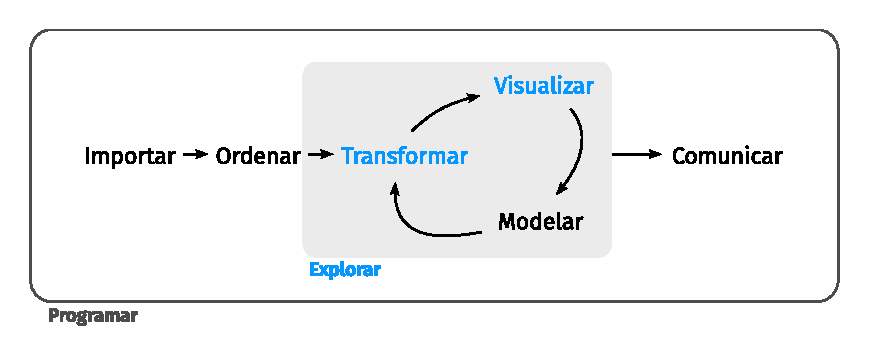
\includegraphics[width=0.75\linewidth]{diagrams_pdf/es/data-science-explore} \end{center}

En esta parte del libro aprenderás algunas herramientas útiles que
tienen un beneficio inmediato: * La visualización es un buen lugar en el
que comenzar a programar en R, ya que el retorno que se obtiene es
claro: puedes crear gráficos elegantes e informativos que te ayuden a
entender los datos. En el capítulo sobre
\protect\hyperlink{visualizaciuxf3n-de-datos}{visualización de datos}
vas a profundizar en este tema y aprenderás la estructura básica de un
gráfico en \textbf{ggplot2},técnicas que te permitirán convertir datos
en gráficos.

\begin{itemize}
\item
  La visualización por sí sola a menudo no es suficiente, por lo que en
  \protect\hyperlink{transform}{transformación de datos} aprenderás los
  verbos clave que te permitirán seleccionar variables importantes,
  filtrar observaciones, crear nuevas variables y calcular estadísticos
  que resuman información.
\item
  Finalmente, en {[}análisis exploratorio de datos (EDA){]} vas a
  combinar visualización y transformación con tu curiosidad y
  escepticismo para formular y responder preguntas en torno a los datos.
\end{itemize}

Si bien modelar es un aspecto importante del proceso exploratorio, aún
no tienes las habilidades para aprenderlo con efectividad o aplicarlo.
Volveremos sobre este tema en el
\protect\hyperlink{model-intro}{capítulo sobre introductorio de
Modelos}, una vez que ya tengas las herramientas de manejo de datos y
programación.

Entre estos tres capítulos que enseñan las herramientas de exploración
de datos hay otros tres capítulos que se enfocan en el flujo de trabajo
en R. En
\protect\hyperlink{flujo-de-trabajo-conocimientos-buxe1sicos}{flujo de
trabajo: conocimientos básicos}, {[}flujo de trabajo: \emph{Scripts}{]}
y {[}flujo de trabajo: proyectos{]} aprenderás buenas prácticas para
escribir y organizar tu código en R. Estas prácticas te prepararán para
el éxito a el largo plazo, en términos de que te entregan las
herramientas necesarias para organizarte cuando abordes proyectos
reales.

\hypertarget{visualizaciuxf3n-de-datos}{%
\chapter{Visualización de datos}\label{visualizaciuxf3n-de-datos}}

\hypertarget{introducciuxf3n-1}{%
\section{Introducción}\label{introducciuxf3n-1}}

\begin{quote}
``Un simple gráfico ha brindado más información a la mente del analista
de datos que cualquier otro dispositivo''. --- John Tukey
\end{quote}

En este capítulo aprenderás cómo visualizar tus datos usando el paquete
\textbf{ggplot2}. De los muchos sistemas que posee R para hacer
gráficos, \textbf{ggplot2} es uno de los más elegantes y versátiles.
Esto se debe a que \textbf{ggplot2} implementa un sistema coherente para
describir y construir gráficos, conocido como la \textbf{gramática de
gráficos}. Con \textbf{ggplot2} puedes hacer más cosas en menor tiempo,
aprendiendo un único sistema y aplicándolo en diferentes ámbitos.

Si deseas obtener más información sobre los fundamentos teóricos de
\textbf{ggplot2} antes de comenzar, te recomendamos leer ``La gramática
de gráficos en capas'',
\url{http://vita.had.co.nz/papers/layered-grammar.pdf}.

\hypertarget{prerrequisitos-1}{%
\subsection{Prerrequisitos}\label{prerrequisitos-1}}

Este capítulo se centra en \textbf{ggplot2}, uno de los paquetes
principales del Tidyverse. Para acceder a sus funciones y las páginas de
ayuda que utilizaremos en este capítulo, debes cargar el Tidyverse
ejecutando este código:

\begin{Shaded}
\begin{Highlighting}[]
\KeywordTok{library}\NormalTok{(tidyverse)}
\end{Highlighting}
\end{Shaded}

Esa única línea de código carga el núcleo del Tidyverse, que está
compuesto por los paquetes que usarás en casi todos tus análisis de
datos. Al correr esta línea también verás cuáles funciones de tidyverse
pueden tener conflicto con funciones de R base (o de otros paquetes que
puedas haber cargado previamente).

Si ejecutas este código y recibes el mensaje de error ``Error in
library(tidyverse): there is no package called `tidyverse'\,'' (no hay
ningún paquete llamado `tidyverse'), primero deberás instalarlo y luego
ejecutar \texttt{library()}:.

\begin{Shaded}
\begin{Highlighting}[]
\KeywordTok{install.packages}\NormalTok{(}\StringTok{"tidyverse"}\NormalTok{)}
\KeywordTok{library}\NormalTok{(tidyverse)}
\end{Highlighting}
\end{Shaded}

Solo es necesario que instales los paquetes una única vez; sin embargo,
tendrás que cargarlos siempre que inicies una nueva sesión.

Cuando necesitemos especificar la procedencia de una función (o un
conjunto de datos), usaremos el formato especial
\texttt{paquete::funcion()}. Por ejemplo, \texttt{ggplot2::ggplot()}
dice explícitamente que estamos usando la función \texttt{ggplot()} del
paquete ggplot2.

Además del Tidyverse, es necesario que cargue el paquete \texttt{datos},
ya que en él están contenidas las versiones en español de los datos que
utilizaremos en este capítulo:

\begin{Shaded}
\begin{Highlighting}[]
\CommentTok{# install.packages("remotes")}
\CommentTok{# remotes::install_github("cienciadedatos/datos")}
\KeywordTok{library}\NormalTok{(datos)}
\end{Highlighting}
\end{Shaded}

\hypertarget{primeros-pasos}{%
\section{Primeros pasos}\label{primeros-pasos}}

Usemos nuestro primer gráfico para responder una pregunta: ¿los
automóviles con motores grandes consumen más combustible que los
automóviles con motores pequeños? Probablemente ya tengas una respuesta,
pero trata de responder de forma precisa. ¿Cómo es la relación entre el
tamaño del motor y la eficiencia del combustible? ¿Es positiva? ¿Es
negativa? ¿Es lineal o no lineal?

\hypertarget{el-data-frame-millas}{%
\subsection{\texorpdfstring{El \emph{data frame}
\texttt{millas}}{El data frame millas}}\label{el-data-frame-millas}}

Puedes poner a prueba tu respuesta empleando el \emph{data frame}
\texttt{millas} que se encuentra en el paquete \textbf{datos}
(\texttt{datos::millas}). Un \emph{data frame} es una colección
rectangular de variables (columnas) y observaciones (filas). El
\emph{data frame} \texttt{millas} contiene observaciones para 38 modelos
de automóviles recopiladas por la Agencia de Protección Ambiental de los
EE. UU.

\begin{Shaded}
\begin{Highlighting}[]
\NormalTok{millas}
\CommentTok{#> # A tibble: 234 x 11}
\CommentTok{#>   fabricante modelo cilindrada  anio cilindros transmision traccion ciudad}
\CommentTok{#>   <chr>      <chr>       <dbl> <int>     <int> <chr>       <chr>     <int>}
\CommentTok{#> 1 audi       a4            1.8  1999         4 auto(l5)    d            18}
\CommentTok{#> 2 audi       a4            1.8  1999         4 manual(m5)  d            21}
\CommentTok{#> 3 audi       a4            2    2008         4 manual(m6)  d            20}
\CommentTok{#> 4 audi       a4            2    2008         4 auto(av)    d            21}
\CommentTok{#> 5 audi       a4            2.8  1999         6 auto(l5)    d            16}
\CommentTok{#> 6 audi       a4            2.8  1999         6 manual(m5)  d            18}
\CommentTok{#> # ... with 228 more rows, and 3 more variables: autopista <int>,}
\CommentTok{#> #   combustible <chr>, clase <chr>}
\end{Highlighting}
\end{Shaded}

Entre las variables de \texttt{millas} se encuentran:

\begin{enumerate}
\def\labelenumi{\arabic{enumi}.}
\item
  \texttt{cilindrada}: tamaño del motor del automóvil, en litros.
\item
  \texttt{autopista}: eficiencia del uso de combustible de un automóvil
  en carretera, en millas por galón. Al recorrer la misma distancia, un
  automóvil de baja eficiencia consume más combustible que un automóvil
  de alta eficiencia.
\end{enumerate}

Para obtener más información sobre el \emph{data frame} \texttt{millas},
abre su página de ayuda ejecutando \texttt{?millas}.

\hypertarget{creando-un-gruxe1fico-con-ggplot}{%
\subsection{Creando un gráfico con
ggplot}\label{creando-un-gruxe1fico-con-ggplot}}

Para graficar \texttt{millas}, ejecuta este código para poner
\texttt{cilindrada} en el eje \texttt{x} y \texttt{autopista} en el eje
\texttt{y}:

\begin{Shaded}
\begin{Highlighting}[]
\KeywordTok{ggplot}\NormalTok{(}\DataTypeTok{data =}\NormalTok{ millas) }\OperatorTok{+}
\StringTok{  }\KeywordTok{geom_point}\NormalTok{(}\DataTypeTok{mapping =} \KeywordTok{aes}\NormalTok{(}\DataTypeTok{x =}\NormalTok{ cilindrada, }\DataTypeTok{y =}\NormalTok{ autopista))}
\end{Highlighting}
\end{Shaded}

\begin{center}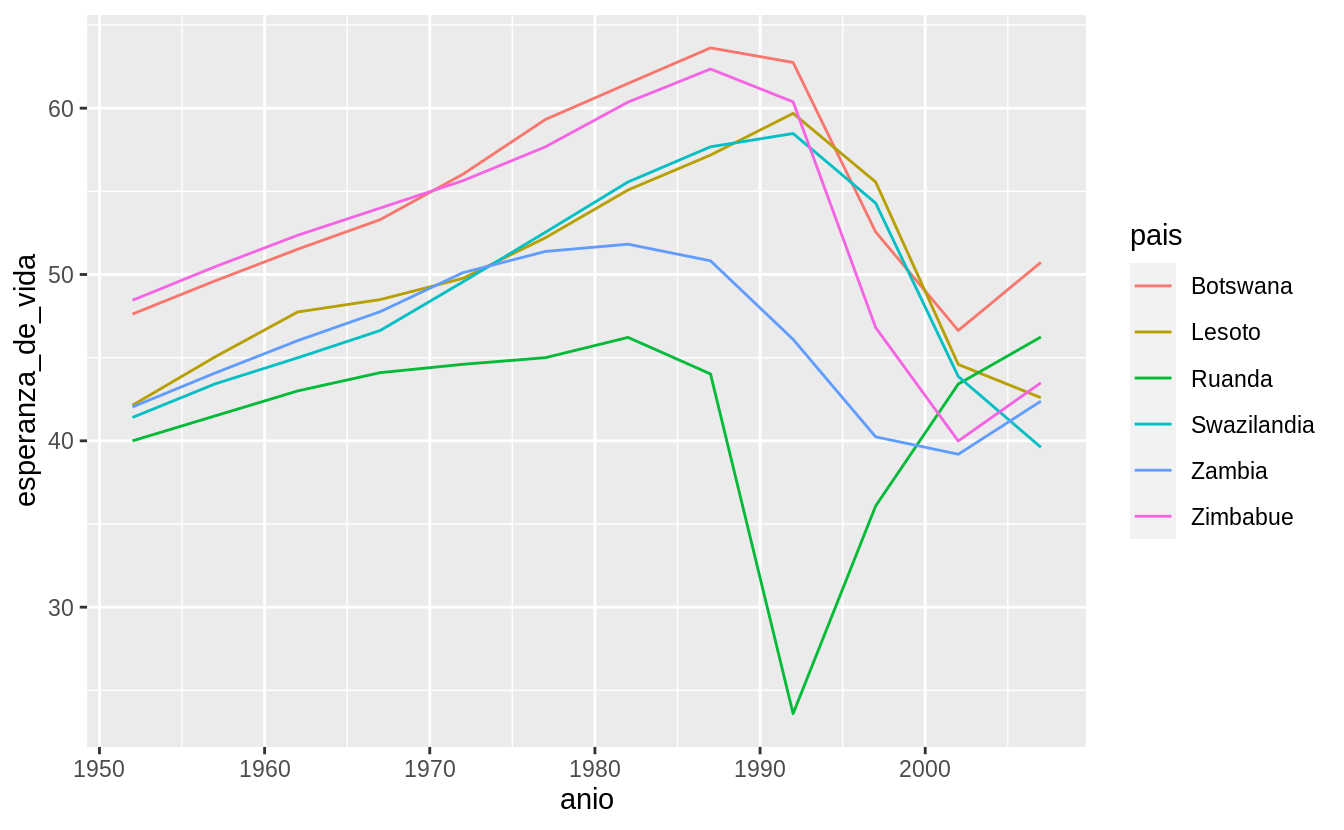
\includegraphics[width=0.7\linewidth]{book_figures/unnamed-chunk-19-1} \end{center}

El gráfico muestra una relación negativa entre el tamaño del motor
(\texttt{cilindrada}) y la eficiencia del combustible
(\texttt{autopista}). En otras palabras, los vehículos con motores
grandes usan más combustible. Este resultado, ¿confirma o refuta tu
hipótesis acerca de la relación entre la eficiencia del combustible y el
tamaño del motor?

Para comenzar un gráfico con \textbf{ggplot2} se utiliza la función
\texttt{ggplot()}. \texttt{ggplot()} crea un sistema de coordenadas al
que puedes agregar capas. El primer argumento de \texttt{ggplot()} es el
conjunto de datos que se utilizará en el gráfico. Si corres
\texttt{ggplot(data\ =\ millas)}, obtendrás un gráfico vacío. Como no es
muy interesante, no vamos a mostrarlo aquí.

Para completar tu gráfico debes agregar una o más capas a
\texttt{ggplot()}. La función \texttt{geom\_point()} agrega una capa de
puntos al gráfico, que crea un diagrama de dispersión (o
\emph{scatterplot}). \textbf{ggplot2} incluye muchas funciones
\emph{geom}, cada una de las cuales agrega un tipo de capa diferente a
un gráfico. Aprenderás muchas de ellas a lo largo de este capítulo.

Cada función geom en \textbf{ggplot2} tiene un argumento de
\texttt{mapping}. Este define cómo se ``mapean'' o se asignan las
variables del conjunto de datos a propiedades visuales. El argumento de
\texttt{mapping} siempre aparece emparejado con \texttt{aes()} y los
argumentos \texttt{x} e \texttt{y} dentro de \texttt{aes()} especifican
qué variables asignar a estos ejes. \textbf{ggplot2} busca la variable
asignada en el argumento \texttt{data}, en este caso, \texttt{millas}.

\hypertarget{una-plantilla-de-gruxe1ficos}{%
\subsection{Una plantilla de
gráficos}\label{una-plantilla-de-gruxe1ficos}}

Convirtamos ahora este código en una plantilla reutilizable para hacer
gráficos con \textbf{ggplot2}. Para hacer un gráfico, reemplaza las
secciones entre corchetes en el siguiente código con un conjunto de
datos, una función geom o una colección de mapeos.

\begin{Shaded}
\begin{Highlighting}[]
\KeywordTok{ggplot}\NormalTok{(}\DataTypeTok{data =} \OperatorTok{<}\NormalTok{DATOS}\OperatorTok{>}\NormalTok{) }\OperatorTok{+}
\StringTok{  }\ErrorTok{<}\NormalTok{GEOM_FUNCIÓN}\OperatorTok{>}\NormalTok{(}\DataTypeTok{mapping =} \KeywordTok{aes}\NormalTok{(}\OperatorTok{<}\NormalTok{MAPEOS}\OperatorTok{>}\NormalTok{))}
\end{Highlighting}
\end{Shaded}

El resto de este capítulo te mostrará cómo utilizar y adaptar esta
plantilla para crear diferentes tipos de gráficos. Comenzaremos por el
componente \texttt{\textless{}MAPEOS\textgreater{}}

\hypertarget{ejercicios}{%
\subsection{Ejercicios}\label{ejercicios}}

\begin{enumerate}
\def\labelenumi{\arabic{enumi}.}
\item
  Ejecuta \texttt{ggplot(data\ =\ millas)}. ¿Qué observas?
\item
  ¿Cuántas filas hay en \texttt{millas}? ¿Cuántas columnas?
\item
  ¿Qué describe la variable \texttt{traccion}? Lee la ayuda de
  \texttt{?millas} para encontrar la respuesta.
\item
  Realiza un gráfico de dispersión de \texttt{autopista} versus
  \texttt{cilindros}.
\item
  ¿Qué sucede cuando haces un gráfico de dispersión (\emph{scatterplot})
  de \texttt{clase} versus \texttt{traccion}? ¿Por qué no es útil este
  gráfico?
\end{enumerate}

\hypertarget{mapeos-estuxe9ticos}{%
\section{Mapeos estéticos}\label{mapeos-estuxe9ticos}}

\begin{quote}
``El mayor valor de una imagen es cuando nos obliga a observar lo que no
esperábamos ver''. --- John Tukey
\end{quote}

En el siguiente gráfico, un grupo de puntos (resaltados en rojo) parece
quedar fuera de la tendencia lineal. Estos automóviles tienen un
kilometraje mayor de lo que esperaríamos. ¿Cómo puedes explicar estos
vehículos?

\begin{center}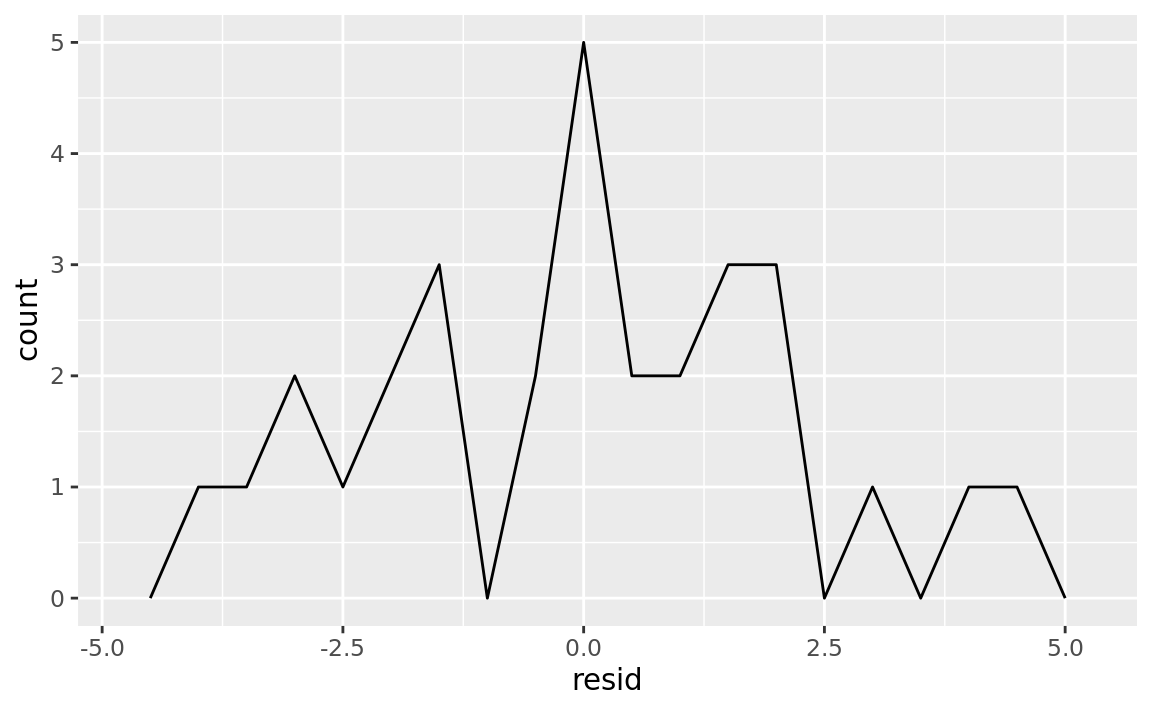
\includegraphics[width=0.7\linewidth]{book_figures/unnamed-chunk-21-1} \end{center}

Supongamos que estos automóviles son híbridos. Una forma de probar esta
hipótesis es observando la variable que indica la \texttt{clase} de cada
automóvil. La variable \texttt{clase} del conjunto de datos de
\texttt{millas} clasifica los autos en grupos como compacto, mediano y
SUV. Si los puntos periféricos corresponden a automóviles híbridos,
deberían estar clasificados como compactos o, tal vez, subcompactos (ten
en cuenta que estos datos se recopilaron antes de que las camionetas
híbridas y SUV se hicieran populares).

Puedes agregar una tercera variable, como \texttt{clase}, a un diagrama
de dispersión bidimensional asignándolo a un parámetro
\textbf{estético}. Un parámetro estético (o \emph{estética}) es una
propiedad visual de los objetos de un gráfico. Las estéticas incluye
cosas como el tamaño, la forma o el color de tus puntos. Puedes mostrar
un punto (como el siguiente) de diferentes maneras si cambias los
valores de sus propiedades estéticas. Como ya usamos la palabra
``valor'' para describir los datos, usemos la palabra ``nivel'' para
describir las propiedades estéticas. Aquí cambiamos los niveles del
tamaño, la forma y el color de un punto para que el punto sea pequeño,
triangular o azul:

\begin{center}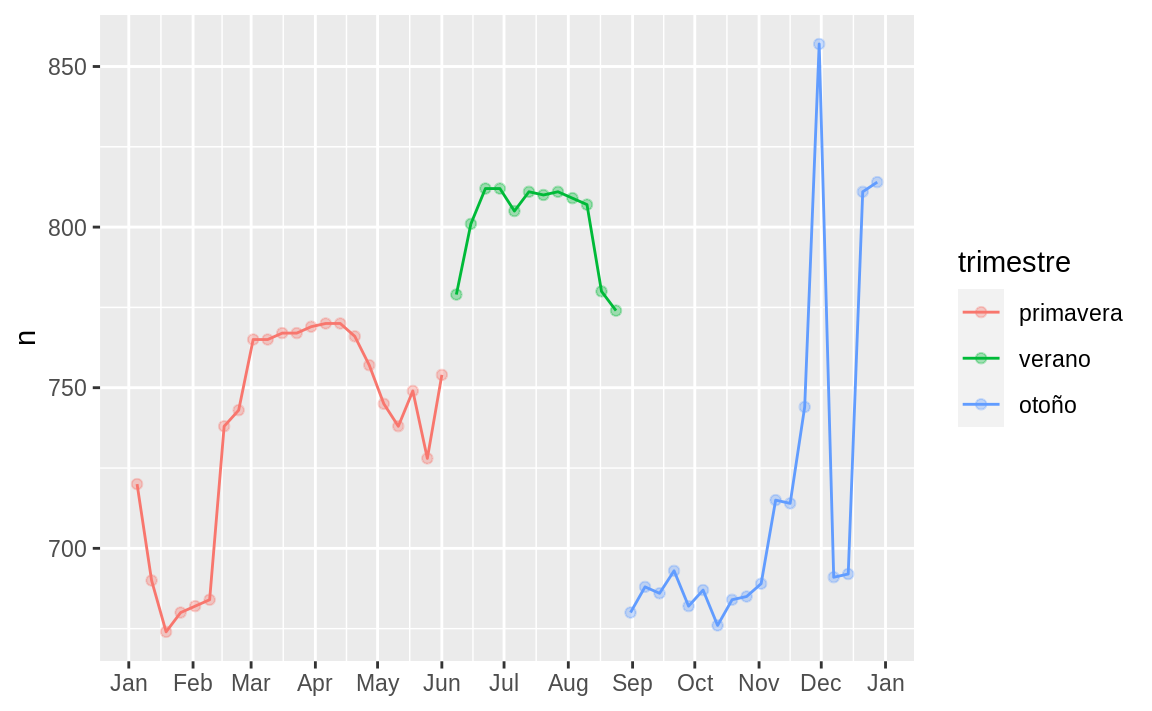
\includegraphics[width=0.7\linewidth]{book_figures/unnamed-chunk-22-1} \end{center}

El mapeo entre las propiedades estéticas de tu gráfico y las variables
de tu \emph{dataset} te permite comunicar información sobre tus datos.
Por ejemplo, puedes asignar los colores de los puntos de acuerdo a la
variable \texttt{clase} para indicar a qué clase pertenece cada
automóvil.

\begin{Shaded}
\begin{Highlighting}[]
\KeywordTok{ggplot}\NormalTok{(}\DataTypeTok{data =}\NormalTok{ millas) }\OperatorTok{+}
\StringTok{  }\KeywordTok{geom_point}\NormalTok{(}\DataTypeTok{mapping =} \KeywordTok{aes}\NormalTok{(}\DataTypeTok{x =}\NormalTok{ cilindrada, }\DataTypeTok{y =}\NormalTok{ autopista, }\DataTypeTok{color =}\NormalTok{ clase))}
\end{Highlighting}
\end{Shaded}

\begin{center}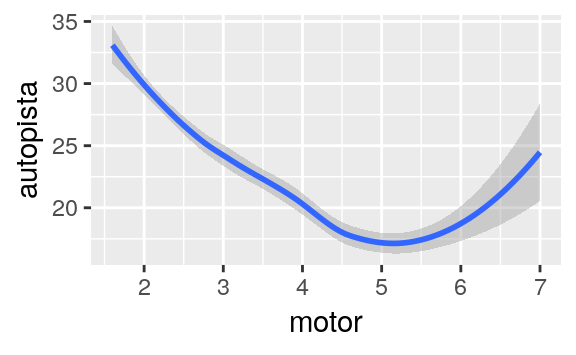
\includegraphics[width=0.7\linewidth]{book_figures/unnamed-chunk-23-1} \end{center}

(Si prefieres el inglés británico, como Hadley, puedes usar
\texttt{colour} en lugar de \texttt{color}).

Para mapear (o asignar) una estética a una variable, debes asociar el
nombre de la estética al de la variable dentro de \texttt{aes()}.
\textbf{ggplot2} asignará automáticamente un nivel único de la estética
(en este ejemplo, un color) a cada valor único de la variable. Este
proceso es conocido como \textbf{escalamiento} (\emph{scaling}).
\textbf{ggplot2} acompañará el gráfico con una leyenda que explica qué
niveles corresponden a qué valores.

Los colores revelan que muchos de los puntos inusuales son automóviles
de dos asientos. ¡Estos no parecen híbridos y son, de hecho, automóviles
deportivos! Los automóviles deportivos tienen motores grandes, como las
camionetas todo terreno o \emph{pickups}, pero su cuerpo es pequeño,
como los automóviles medianos y compactos, lo que mejora su consumo de
gasolina. En retrospectiva, es poco probable que estos automóviles sean
híbridos, ya que tienen motores grandes.

En el ejemplo anterior asignamos la variable \texttt{clase} a la
estética de color, pero podríamos haberla asignado a la estética del
tamaño del mismo modo. En este caso, el tamaño exacto de cada punto
revelaría a qué clase pertenece. Recibimos aquí una \textbf{advertencia}
(\emph{warning}), porque mapear una variable no ordenada
(\texttt{clase}) a una estética ordenada (\texttt{size}) no es una buena
idea.

\begin{Shaded}
\begin{Highlighting}[]
\KeywordTok{ggplot}\NormalTok{(}\DataTypeTok{data =}\NormalTok{ millas) }\OperatorTok{+}
\StringTok{  }\KeywordTok{geom_point}\NormalTok{(}\DataTypeTok{mapping =} \KeywordTok{aes}\NormalTok{(}\DataTypeTok{x =}\NormalTok{ cilindrada, }\DataTypeTok{y =}\NormalTok{ autopista, }\DataTypeTok{size =}\NormalTok{ clase))}
\end{Highlighting}
\end{Shaded}

\begin{center}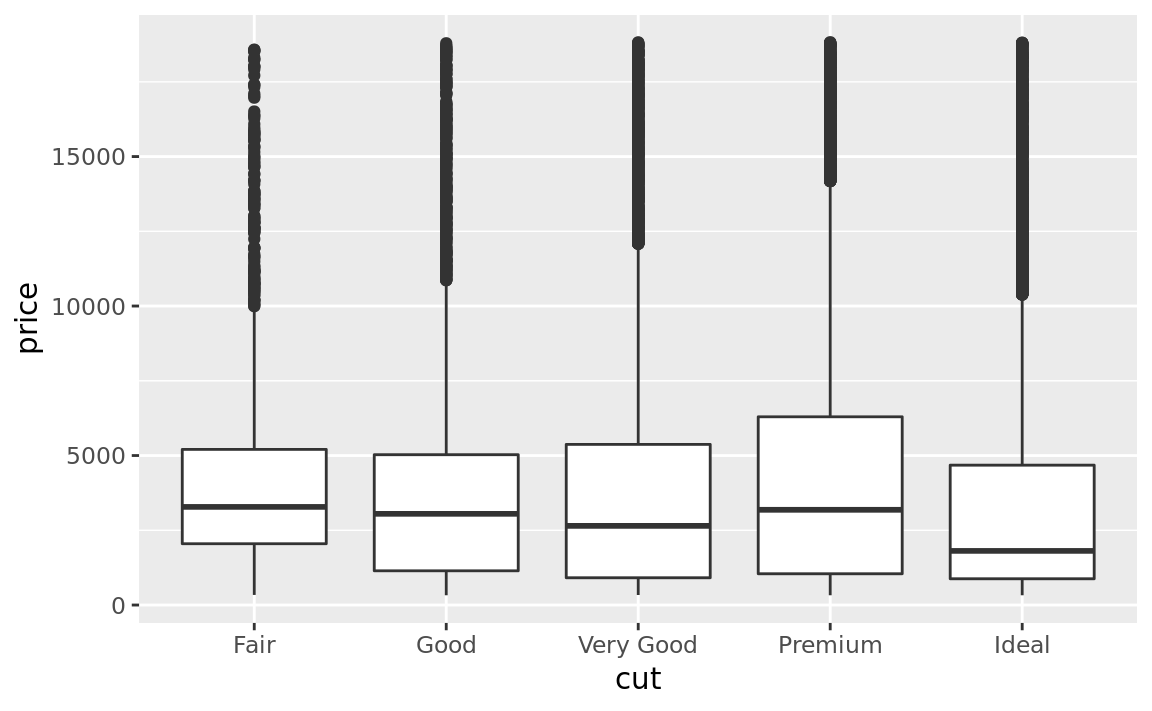
\includegraphics[width=0.7\linewidth]{book_figures/unnamed-chunk-24-1} \end{center}

También podríamos haber asignado la variable \texttt{clase} a la
estética \emph{alpha}, que controla la transparencia de los puntos, o a
la estética \emph{shape} que controla la forma (\emph{shape}) de los
puntos.

\begin{Shaded}
\begin{Highlighting}[]
\CommentTok{# Izquierda}
\KeywordTok{ggplot}\NormalTok{(}\DataTypeTok{data =}\NormalTok{ millas) }\OperatorTok{+}
\StringTok{  }\KeywordTok{geom_point}\NormalTok{(}\DataTypeTok{mapping =} \KeywordTok{aes}\NormalTok{(}\DataTypeTok{x =}\NormalTok{ cilindrada, }\DataTypeTok{y =}\NormalTok{ autopista, }\DataTypeTok{alpha =}\NormalTok{ clase))}

\CommentTok{# Derecha}
\KeywordTok{ggplot}\NormalTok{(}\DataTypeTok{data =}\NormalTok{ millas) }\OperatorTok{+}
\StringTok{  }\KeywordTok{geom_point}\NormalTok{(}\DataTypeTok{mapping =} \KeywordTok{aes}\NormalTok{(}\DataTypeTok{x =}\NormalTok{ cilindrada, }\DataTypeTok{y =}\NormalTok{ autopista, }\DataTypeTok{shape =}\NormalTok{ clase))}
\end{Highlighting}
\end{Shaded}

\begin{figure}
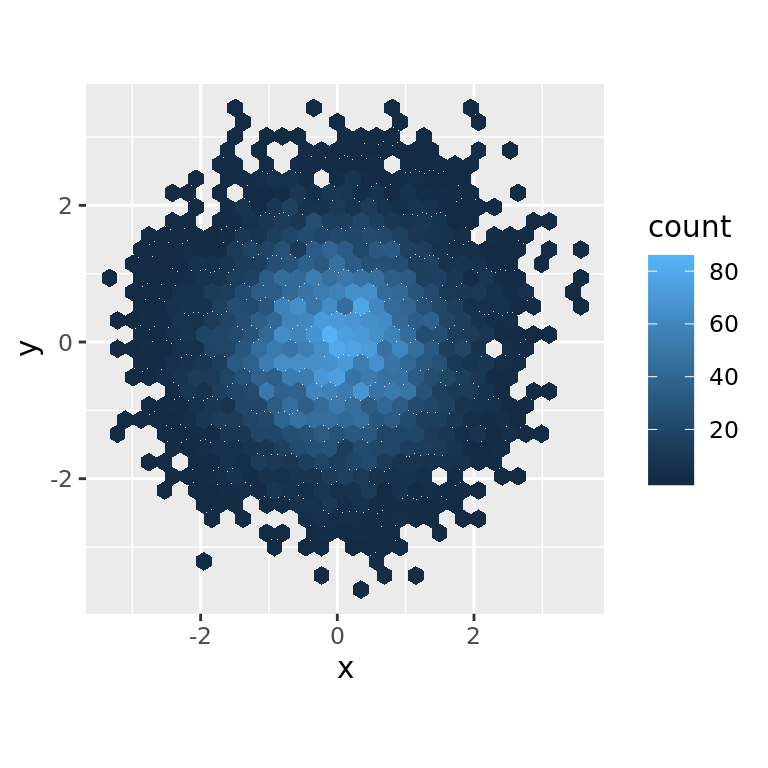
\includegraphics[width=0.5\linewidth]{book_figures/unnamed-chunk-25-1} 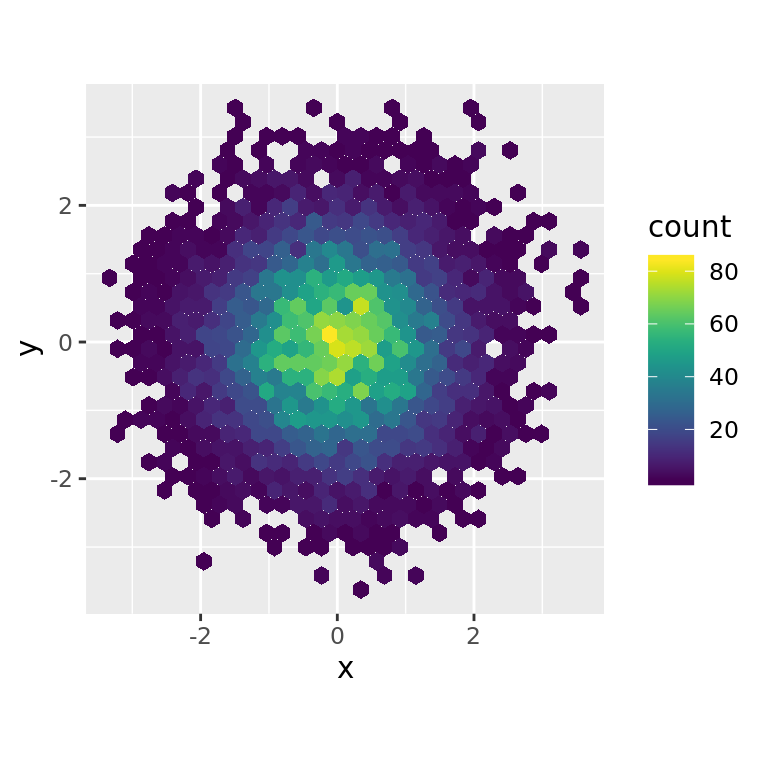
\includegraphics[width=0.5\linewidth]{book_figures/unnamed-chunk-25-2} \end{figure}

¿Qué pasó con los SUV? \textbf{ggplot2} solo puede usar seis formas a la
vez. De forma predeterminada, los grupos adicionales no se grafican
cuando se emplea la estética de la forma (\emph{shape}).

Para cada estética utilizamos \texttt{aes()} para asociar su nombre con
la variable seleccionada para graficar. La función \texttt{aes()} reúne
cada una de las asignaciones estéticas utilizadas por una capa y las
pasa al argumento de mapeo de la capa. La sintaxis resalta una visión
útil sobre \texttt{x} e \texttt{y}: las ubicaciones de x e y de un punto
son en sí mismas también estéticas, es decir propiedades visuales que se
puede asignar a las variables para mostrar información sobre los datos.

Una vez que asignas (o ``mapeas'') una estética, \textbf{ggplot2} se
ocupa del resto. El paquete selecciona una escala razonable para usar
con la estética elegida y construye una leyenda que explica la relación
entre niveles y valores. Para la estética \texttt{x} e \texttt{y},
\textbf{ggplot2} no crea una leyenda, pero sí una línea que delimita el
eje con sus marcas de graduación y una etiqueta. La línea del eje actúa
como una leyenda; explica el mapeo entre ubicaciones y valores.

También puedes \emph{fijar} las propiedades estéticas de tu \emph{geom}
manualmente. Por ejemplo, podemos hacer que todos los puntos del gráfico
sean azules:

\begin{Shaded}
\begin{Highlighting}[]
\KeywordTok{ggplot}\NormalTok{(}\DataTypeTok{data =}\NormalTok{ millas) }\OperatorTok{+}
\StringTok{ }\KeywordTok{geom_point}\NormalTok{(}\DataTypeTok{mapping =} \KeywordTok{aes}\NormalTok{(}\DataTypeTok{x =}\NormalTok{ cilindrada, }\DataTypeTok{y =}\NormalTok{ autopista), }\DataTypeTok{color =} \StringTok{"blue"}\NormalTok{)}
\end{Highlighting}
\end{Shaded}

\begin{center}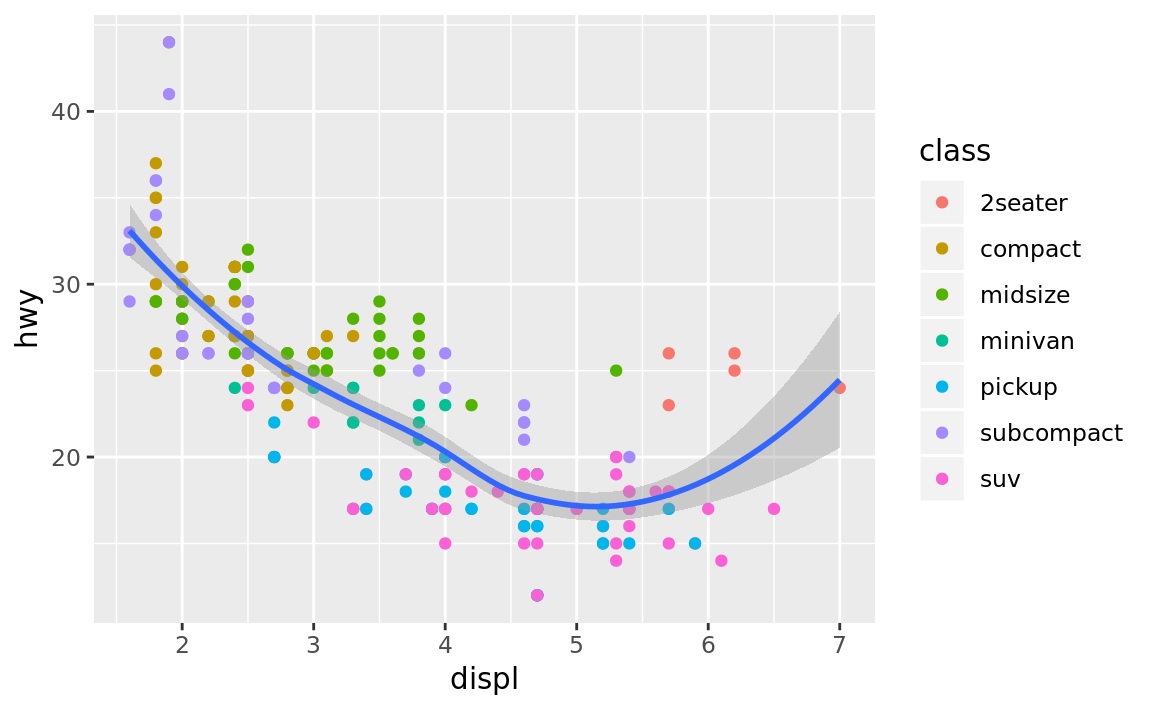
\includegraphics[width=0.7\linewidth]{book_figures/unnamed-chunk-26-1} \end{center}

Aquí, el color no transmite información sobre una variable, sino que
cambia la apariencia del gráfico. Para establecer una estética de forma
manual, debes usar el nombre de la estética como un argumento de la
función geom; es decir, va \emph{fuera} de \texttt{aes()}. Tendrás que
elegir un nivel que tenga sentido para esa estética:

\begin{itemize}
\item
  El nombre de un color como cadena de caracteres.
\item
  El tamaño de un punto en mm.
\item
  La forma de un punto como un número, tal como se muestra en la Figura
  @ref(fig:shapes).
\end{itemize}

\begin{figure}

{\centering 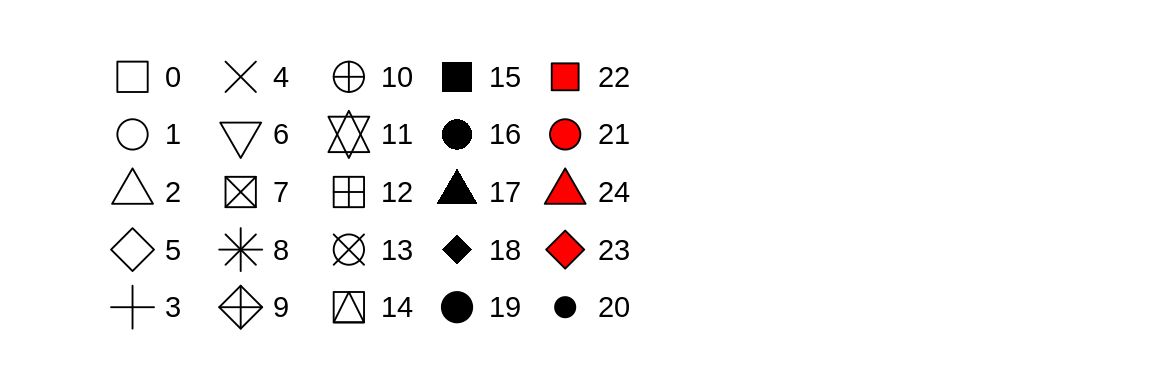
\includegraphics[width=0.75\linewidth]{book_figures/shapes-1} 

}

\caption{R tiene 25 formas predefinidas que están identificadas por números. Hay algunas que parecen duplicados: por ejemplo 0, 15 y 22 son todos cuadrados. La diferencia viene de la interacción entre las estéticas `color` y `fill` (*relleno*). Las formas vacías (0--14) tienen un borde determinado por `color`; las formas sólidas (15--18) están rellenas con `color`; las formas rellenas (21--24) tienen un borde de `color` y están rellenas por `fill`.}\label{fig:shapes}
\end{figure}

\hypertarget{ejercicios-1}{%
\subsection{Ejercicios}\label{ejercicios-1}}

\begin{enumerate}
\def\labelenumi{\arabic{enumi}.}
\tightlist
\item
  ¿Qué no va bien en este código? ¿Por qué hay puntos que no son azules?
\end{enumerate}

\begin{Shaded}
\begin{Highlighting}[]
 \KeywordTok{ggplot}\NormalTok{(}\DataTypeTok{data =}\NormalTok{ millas) }\OperatorTok{+}
\StringTok{   }\KeywordTok{geom_point}\NormalTok{(}\DataTypeTok{mapping =} \KeywordTok{aes}\NormalTok{(}\DataTypeTok{x =}\NormalTok{ cilindrada, }\DataTypeTok{y =}\NormalTok{ autopista, }\DataTypeTok{color =} \StringTok{"blue"}\NormalTok{))}
\end{Highlighting}
\end{Shaded}

\begin{center}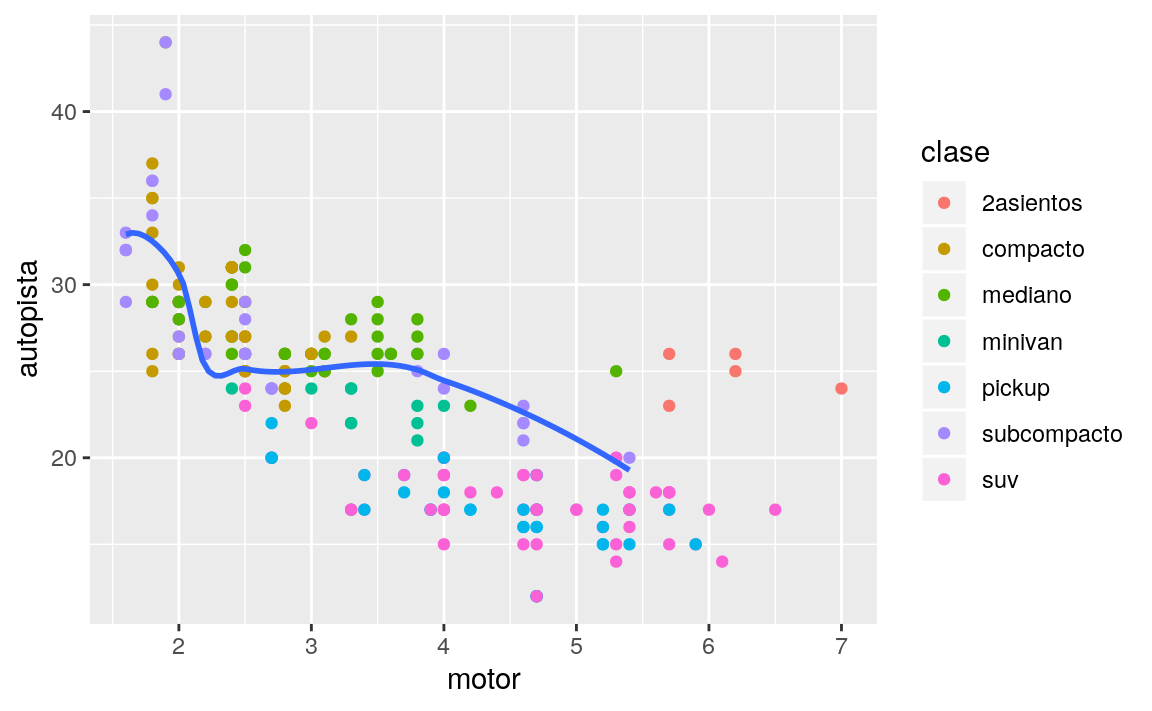
\includegraphics[width=0.7\linewidth]{book_figures/unnamed-chunk-27-1} \end{center}

\begin{enumerate}
\def\labelenumi{\arabic{enumi}.}
\setcounter{enumi}{1}
\item
  ¿Qué variables en \texttt{millas} son categóricas? ¿Qué variables son
  continuas? (Pista: escribe \texttt{?millas} para leer la documentación
  de ayuda para este conjunto de datos). ¿Cómo puedes ver esta
  información cuando ejecutas \texttt{millas}?
\item
  Asigna una variable continua a \texttt{color}, \texttt{size}, y
  \texttt{shape}. ¿Cómo se comportan estas estéticas de manera diferente
  para variables categóricas y variables continuas?
\item
  ¿Qué ocurre si asignas o mapeas la misma variable a múltiples
  estéticas?
\item
  ¿Qué hace la estética \texttt{stroke}? ¿Con qué formas trabaja?
  (Pista: consulta \texttt{?geom\_point})
\item
  ¿Qué ocurre si se asigna o mapea una estética a algo diferente del
  nombre de una variable, como
  \texttt{aes(color\ =\ cilindrada\ \textless{}\ 5)}?
\end{enumerate}

\hypertarget{problemas-comunes}{%
\section{Problemas comunes}\label{problemas-comunes}}

A medida que empieces a escribir código en R, lo más probable es que te
encuentres con problemas. No te preocupes, es lo más común. Hemos estado
escribiendo código en R durante años, ¡y todos los días seguimos
escribiendo código que no funciona!

Comienza comparando cuidadosamente el código que estás ejecutando con el
código en este libro. R es extremadamente exigente y un carácter fuera
de lugar puede marcar la diferencia. Asegúrate de que cada \texttt{(}
coincida con un \texttt{)} y cada \texttt{"} esté emparejado con
otro\texttt{"}. Algunas veces ejecutarás el código y no pasará nada.
Comprueba la parte izquierda de tu consola: si es un \texttt{+},
significa que R no cree que hayas escrito una expresión completa y está
esperando que la termines. En este caso, normalmente es más fácil
comenzar de nuevo desde cero presionando ESCAPE (la tecla \emph{esc})
para cancelar el procesamiento del comando actual.

Un problema común al crear gráficos con \textbf{ggplot2} es colocar el
\texttt{+} en el lugar equivocado: debe ubicarse al final de la línea,
no al inicio. En otras palabras, asegúrate de no haber escrito
accidentalmente un código como este:

\begin{Shaded}
\begin{Highlighting}[]
\KeywordTok{ggplot}\NormalTok{(}\DataTypeTok{data =}\NormalTok{ millas)}
\OperatorTok{+}\StringTok{ }\KeywordTok{geom_point}\NormalTok{(}\DataTypeTok{mapping =} \KeywordTok{aes}\NormalTok{(}\DataTypeTok{x =}\NormalTok{ cilindrada, }\DataTypeTok{y =}\NormalTok{ autopista))}
\end{Highlighting}
\end{Shaded}

Si esto no resuelve el problema, prueba con la ayuda. Puedes obtener
ayuda sobre cualquier función R ejecutando
\texttt{?nombre\_de\_la\_funcion} en la consola o seleccionando el
nombre de la función y presionando F1 en RStudio. No te preocupes si la
ayuda no te parece tan útil, trata entonces de saltar a los ejemplos y
buscar un pedazo de código que coincida con lo que intentas hacer.

Si eso no ayuda, lee cuidadosamente el mensaje de error. ¡A veces la
respuesta estará oculta allí! Sin embargo, cuando recién comienzas en R,
puede que la respuesta esté en el mensaje de error, pero aún no sabes
cómo entenderlo. Otra gran herramienta es Google: intenta buscar allí el
mensaje de error, ya que es probable que otra persona haya tenido el
mismo problema y haya obtenido ayuda en línea.

\hypertarget{separar-en-facetas}{%
\section{Separar en facetas}\label{separar-en-facetas}}

Una forma de agregar variables adicionales es con las estéticas. Otra
forma particularmente útil para las variables categóricas consiste en
dividir el gráfico en \textbf{facetas}, es decir, sub-gráficos que
muestran cada uno un subconjunto de los datos.

Para separar en facetas un gráfico según una sola variable, utiliza
\texttt{facet\_wrap()} (del inglés \emph{envolver una faceta}). El
primer argumento de \texttt{facet\_wrap()} debería ser una fórmula
creada con \texttt{\textasciitilde{}} seguido del nombre de una de las
variable (aquí ``fórmula'' es el nombre de un tipo de estructura en R,
no un sinónimo de ``ecuación''). La variable que uses en
\texttt{facet\_wrap()} debe ser categórica.

\begin{Shaded}
\begin{Highlighting}[]
\KeywordTok{ggplot}\NormalTok{(}\DataTypeTok{data =}\NormalTok{ millas) }\OperatorTok{+}
\StringTok{  }\KeywordTok{geom_point}\NormalTok{(}\DataTypeTok{mapping =} \KeywordTok{aes}\NormalTok{(}\DataTypeTok{x =}\NormalTok{ cilindrada, }\DataTypeTok{y =}\NormalTok{ autopista)) }\OperatorTok{+}
\StringTok{  }\KeywordTok{facet_wrap}\NormalTok{(}\OperatorTok{~}\StringTok{ }\NormalTok{clase, }\DataTypeTok{nrow =} \DecValTok{2}\NormalTok{)}
\end{Highlighting}
\end{Shaded}

\begin{center}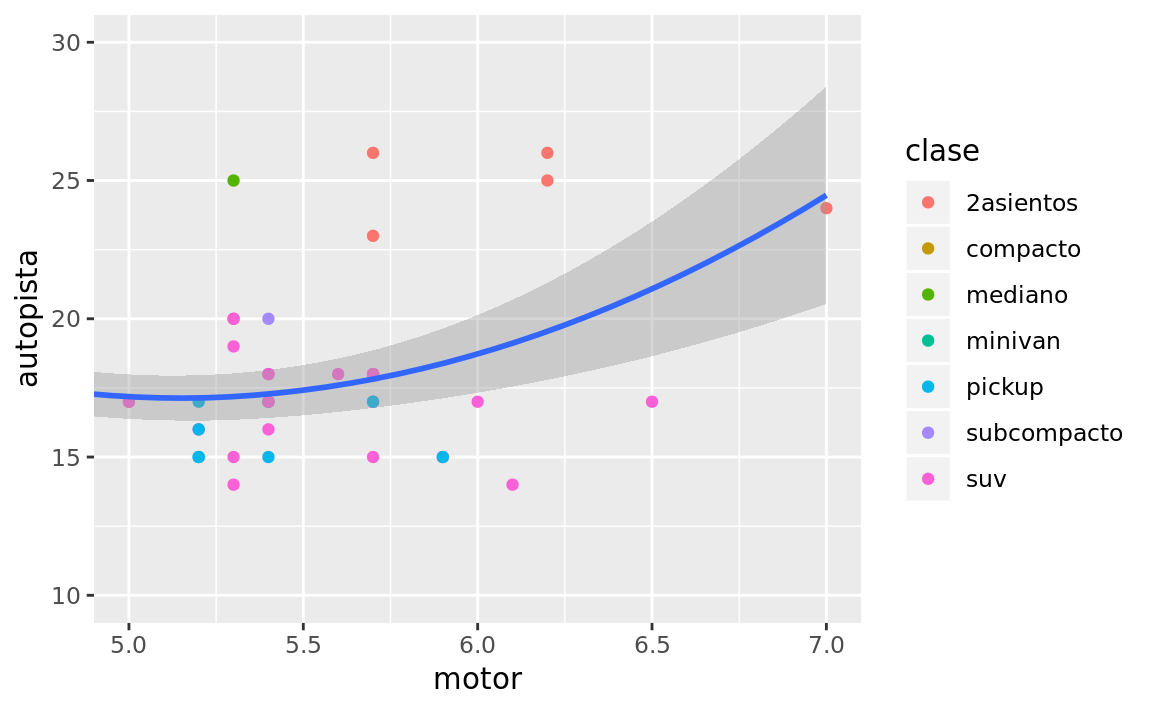
\includegraphics[width=0.7\linewidth]{book_figures/unnamed-chunk-28-1} \end{center}

Para separar en facetas un gráfico según las combinaciones de dos
variables, agrega \texttt{facet\_grid()} a tu código del gráfico
(\emph{grid} quiere decir cuadrícula en inglés). El primer argumento de
\texttt{facet\_grid()} también corresponde a una fórmula. Esta vez, la
fórmula debe contener dos nombres de variables separados por un
\texttt{\textasciitilde{}}.

\begin{Shaded}
\begin{Highlighting}[]
\KeywordTok{ggplot}\NormalTok{(}\DataTypeTok{data =}\NormalTok{ millas) }\OperatorTok{+}
\StringTok{  }\KeywordTok{geom_point}\NormalTok{(}\DataTypeTok{mapping =} \KeywordTok{aes}\NormalTok{(}\DataTypeTok{x =}\NormalTok{ cilindrada, }\DataTypeTok{y =}\NormalTok{ autopista)) }\OperatorTok{+}
\StringTok{  }\KeywordTok{facet_grid}\NormalTok{(traccion }\OperatorTok{~}\StringTok{ }\NormalTok{cilindros)}
\end{Highlighting}
\end{Shaded}

\begin{center}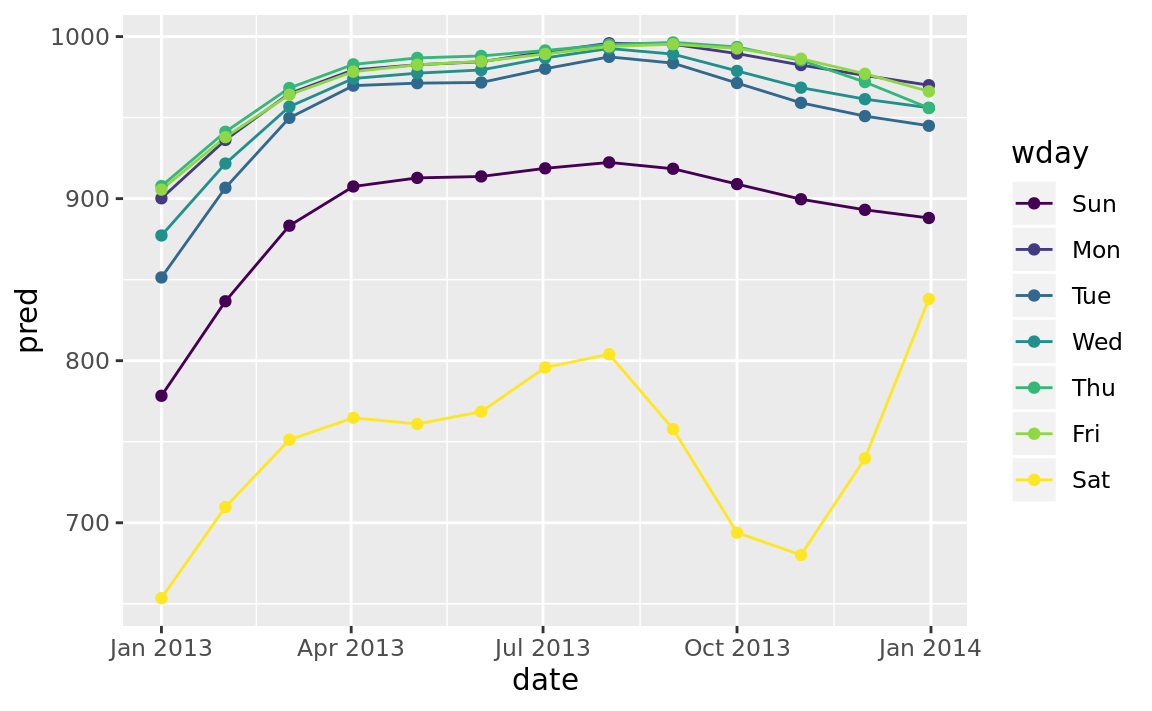
\includegraphics[width=0.7\linewidth]{book_figures/unnamed-chunk-29-1} \end{center}

Si prefieres no separar en facetas las filas o columnas, remplaza por un
\texttt{.} el nombre de alguna de las variables, por ejemplo
\texttt{+\ facet\_grid(.\ \textasciitilde{}\ cilindros)}.

\hypertarget{ejercicios-2}{%
\subsection{Ejercicios}\label{ejercicios-2}}

\begin{enumerate}
\def\labelenumi{\arabic{enumi}.}
\item
  ¿Qué ocurre si intentas separar en facetas una variable continua?
\item
  ¿Qué significan las celdas vacías que aparecen en el gráfico generado
  usando \texttt{facet\_grid(traccion\ \textasciitilde{}\ cilindros)}?
  ¿Cómo se relacionan con este gráfico?

\begin{Shaded}
\begin{Highlighting}[]
\KeywordTok{ggplot}\NormalTok{(}\DataTypeTok{data =}\NormalTok{ millas) }\OperatorTok{+}
\StringTok{  }\KeywordTok{geom_point}\NormalTok{(}\DataTypeTok{mapping =} \KeywordTok{aes}\NormalTok{(}\DataTypeTok{x =}\NormalTok{ traccion, }\DataTypeTok{y =}\NormalTok{ cilindros))}
\end{Highlighting}
\end{Shaded}
\item
  ¿Qué grafica el siguiente código? ¿Qué hace \texttt{.} ?

\begin{Shaded}
\begin{Highlighting}[]
\KeywordTok{ggplot}\NormalTok{(}\DataTypeTok{data =}\NormalTok{ millas) }\OperatorTok{+}
\StringTok{  }\KeywordTok{geom_point}\NormalTok{(}\DataTypeTok{mapping =} \KeywordTok{aes}\NormalTok{(}\DataTypeTok{x =}\NormalTok{ cilindrada, }\DataTypeTok{y =}\NormalTok{ autopista)) }\OperatorTok{+}
\StringTok{  }\KeywordTok{facet_grid}\NormalTok{(traccion }\OperatorTok{~}\StringTok{ }\NormalTok{.)}

\KeywordTok{ggplot}\NormalTok{(}\DataTypeTok{data =}\NormalTok{ millas) }\OperatorTok{+}
\StringTok{  }\KeywordTok{geom_point}\NormalTok{(}\DataTypeTok{mapping =} \KeywordTok{aes}\NormalTok{(}\DataTypeTok{x =}\NormalTok{ cilindrada, }\DataTypeTok{y =}\NormalTok{ autopista)) }\OperatorTok{+}
\StringTok{  }\KeywordTok{facet_grid}\NormalTok{(. }\OperatorTok{~}\StringTok{ }\NormalTok{cilindros)}
\end{Highlighting}
\end{Shaded}
\item
  Mira de nuevo el primer gráfico en facetas presentado en esta sección:

\begin{Shaded}
\begin{Highlighting}[]
\KeywordTok{ggplot}\NormalTok{(}\DataTypeTok{data =}\NormalTok{ millas) }\OperatorTok{+}
\StringTok{  }\KeywordTok{geom_point}\NormalTok{(}\DataTypeTok{mapping =} \KeywordTok{aes}\NormalTok{(}\DataTypeTok{x =}\NormalTok{ cilindrada, }\DataTypeTok{y =}\NormalTok{ autopista)) }\OperatorTok{+}
\StringTok{  }\KeywordTok{facet_wrap}\NormalTok{(}\OperatorTok{~}\StringTok{ }\NormalTok{clase, }\DataTypeTok{nrow =} \DecValTok{2}\NormalTok{)}
\end{Highlighting}
\end{Shaded}

  ¿Cuáles son las ventajas de separar en facetas en lugar de aplicar una
  estética de color? ¿Cuáles son las desventajas? ¿Cómo cambiaría este
  balance si tuvieras un conjunto de datos más grande?
\item
  Lee \texttt{?facet\_wrap}. ¿Qué hace \texttt{nrow}? ¿Qué hace
  \texttt{ncol}? ¿Qué otras opciones controlan el diseño de los paneles
  individuales? ¿Por qué \texttt{facet\_grid()} no tiene argumentos
  \texttt{nrow} y \texttt{ncol}?
\item
  Cuando usas \texttt{facet\_grid()}, generalmente deberías poner la
  variable con un mayor número de niveles únicos en las columnas. ¿Por
  qué?
\end{enumerate}

\hypertarget{objetos-geomuxe9tricos}{%
\section{Objetos geométricos}\label{objetos-geomuxe9tricos}}

¿En qué sentido estos dos gráficos son similares?

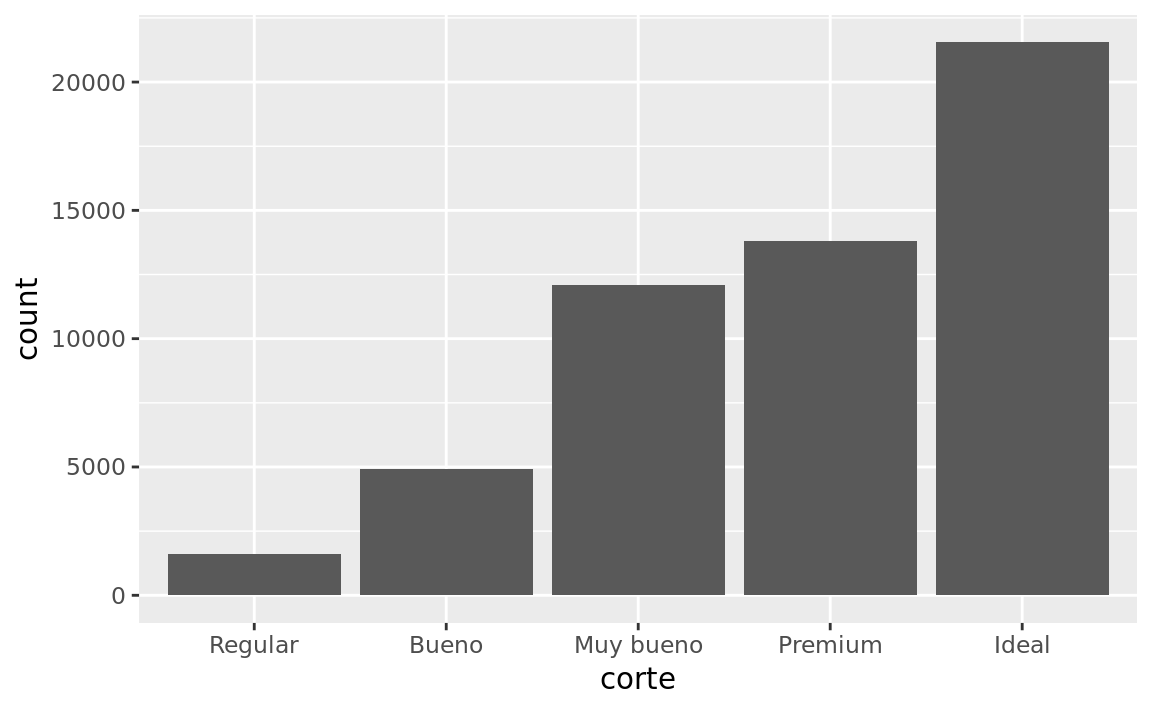
\includegraphics[width=0.5\linewidth]{book_figures/unnamed-chunk-33-1}
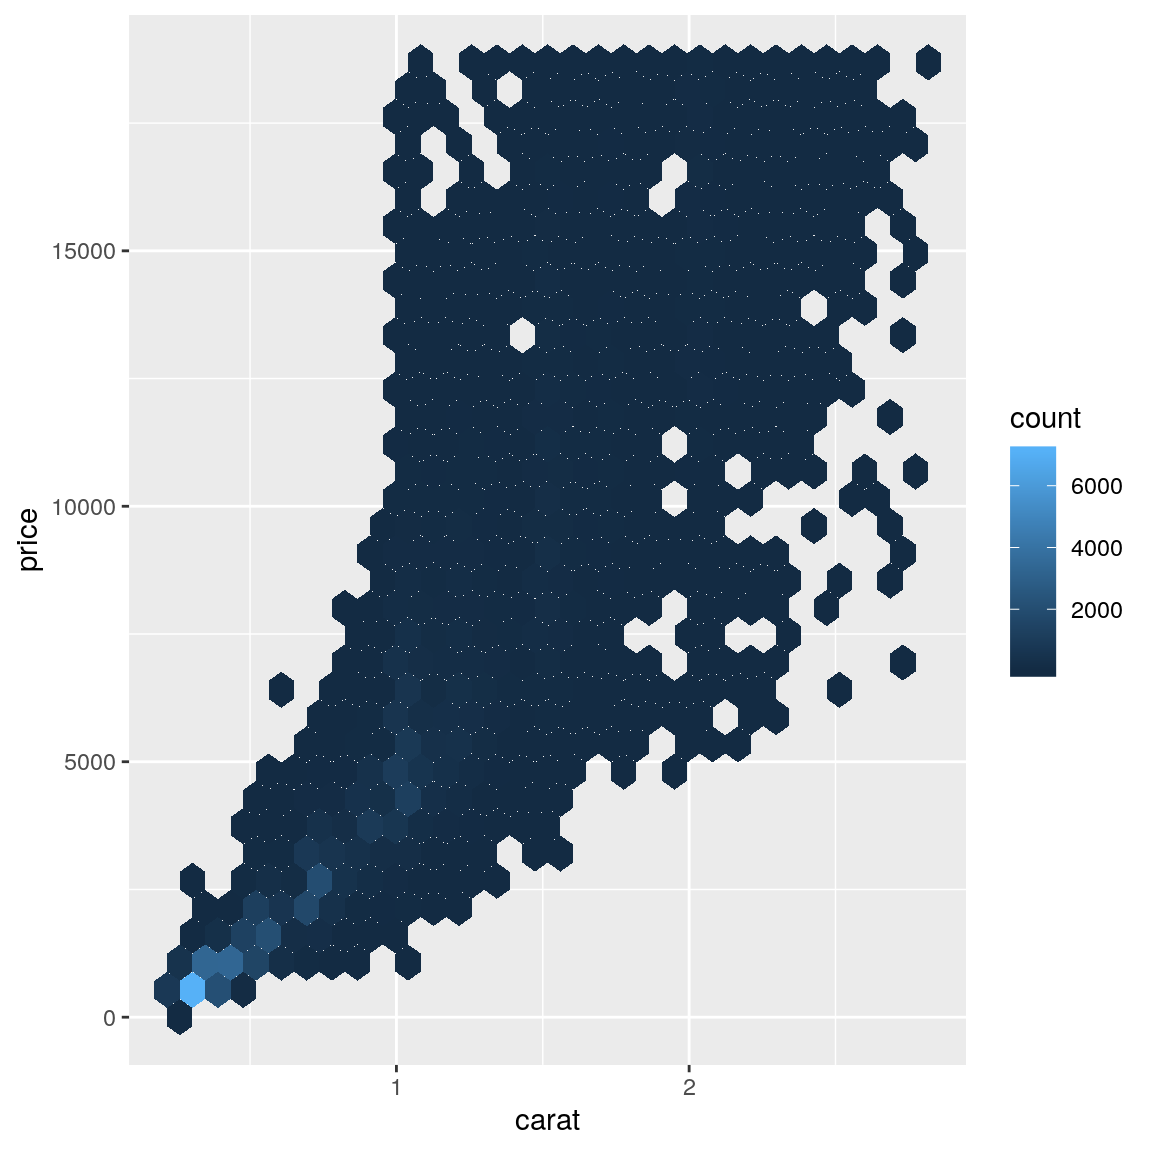
\includegraphics[width=0.5\linewidth]{book_figures/unnamed-chunk-33-2}

Ambos gráficos contienen las mismas variables x e y, y ambos describen
los mismos datos. Pero los gráficos no son idénticos. Cada uno utiliza
un objeto visual diferente para representar los datos. En la sintaxis de
\textbf{ggplot2}, decimos que usan diferentes \textbf{geoms}.

Un \textbf{geom} es el objeto geométrico usado para representar datos de
forma gráfica. La gente a menudo llama a los gráficos por el tipo de
geom que utiliza. Por ejemplo, los diagramas de barras usan geoms de
barra (\emph{bar}), los diagramas de líneas usan geoms de línea
(\emph{line}), los diagramas de caja usan geoms de diagrama de caja
(\emph{boxplot}), y así sucesivamente. En inglés, los diagramas de
puntos (llamados \emph{scatterplots}) rompen la tendencia; ellos usan
geom de punto (o \emph{point}). Como vemos arriba, puedes usar
diferentes geoms para graficar los mismos datos. La gráfica de la
izquierda usa el geom de punto (\texttt{geom\_point()}), y la gráfica de
la derecha usa el geom suavizado (\texttt{geom\_smooth()}), una línea
suavizada ajustada a los datos.

Para cambiar el geom de tu gráfico, modifica la función geom que
acompaña a \texttt{ggplot()}. Por ejemplo, para hacer los gráficos que
se muestran arriba, puedes usar este código:

\begin{Shaded}
\begin{Highlighting}[]
\CommentTok{# izquierda}
\KeywordTok{ggplot}\NormalTok{(}\DataTypeTok{data =}\NormalTok{ millas) }\OperatorTok{+}
\StringTok{  }\KeywordTok{geom_point}\NormalTok{(}\DataTypeTok{mapping =} \KeywordTok{aes}\NormalTok{(}\DataTypeTok{x =}\NormalTok{ cilindrada, }\DataTypeTok{y =}\NormalTok{ autopista))}

\CommentTok{# derecha}
\KeywordTok{ggplot}\NormalTok{(}\DataTypeTok{data =}\NormalTok{ millas) }\OperatorTok{+}
\StringTok{  }\KeywordTok{geom_smooth}\NormalTok{(}\DataTypeTok{mapping =} \KeywordTok{aes}\NormalTok{(}\DataTypeTok{x =}\NormalTok{ cilindrada, }\DataTypeTok{y =}\NormalTok{ autopista))}
\end{Highlighting}
\end{Shaded}

Cada función geom en \textbf{ggplot2} toma un argumento de
\texttt{mapping}. Sin embargo, no todas las estéticas funcionan con
todos los geom. Puedes establecer la forma para un punto, pero no puedes
establecer la ``forma'' de una línea. Por otro lado, para una línea
\emph{podrías} elegir el \emph{tipo} de línea (\emph{linetype}).
\texttt{geom\_smooth()} dibujará una línea diferente, con un tipo de
línea distinto (\emph{linetype}), para cada valor único de la variable
que asignes al tipo de línea (\emph{linetype}).

\begin{Shaded}
\begin{Highlighting}[]
\KeywordTok{ggplot}\NormalTok{(}\DataTypeTok{data =}\NormalTok{ millas) }\OperatorTok{+}
\StringTok{  }\KeywordTok{geom_smooth}\NormalTok{(}\DataTypeTok{mapping =} \KeywordTok{aes}\NormalTok{(}\DataTypeTok{x =}\NormalTok{ cilindrada, }\DataTypeTok{y =}\NormalTok{ autopista, }\DataTypeTok{linetype =}\NormalTok{ traccion))}
\end{Highlighting}
\end{Shaded}

\begin{center}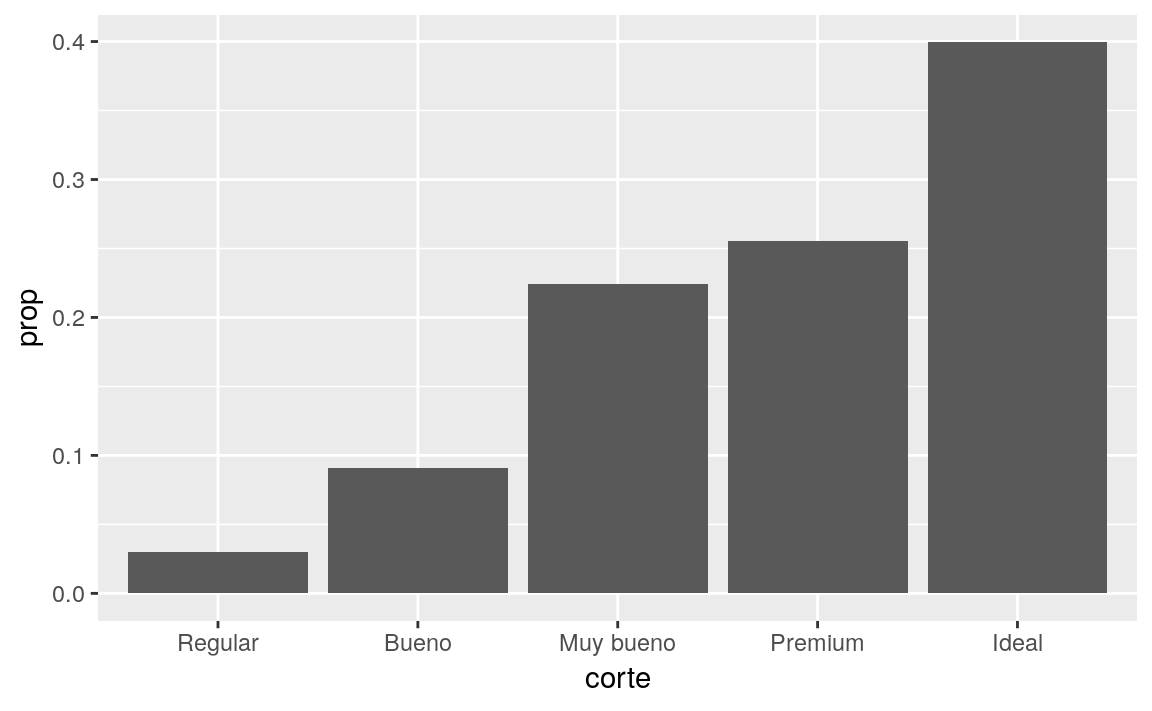
\includegraphics[width=0.7\linewidth]{book_figures/unnamed-chunk-35-1} \end{center}

Aquí \texttt{geom\_smooth()} separa los automóviles en tres líneas en
función de su valor de \texttt{traccion}, que describe el tipo de
transmisión de un automóvil. Una línea describe todos los puntos con un
valor de \texttt{4}, otra línea los de valor \texttt{d}, y una tercera
línea describe los puntos con un valor \texttt{t}. Aquí, \texttt{4}
significa tracción en las cuatro ruedas, \texttt{d} tracción delantera y
\texttt{t} tracción trasera.

Si esto suena extraño, podemos hacerlo más claro al superponer las
líneas sobre los datos brutos y luego colorear todo según
\texttt{traccion}.

\begin{center}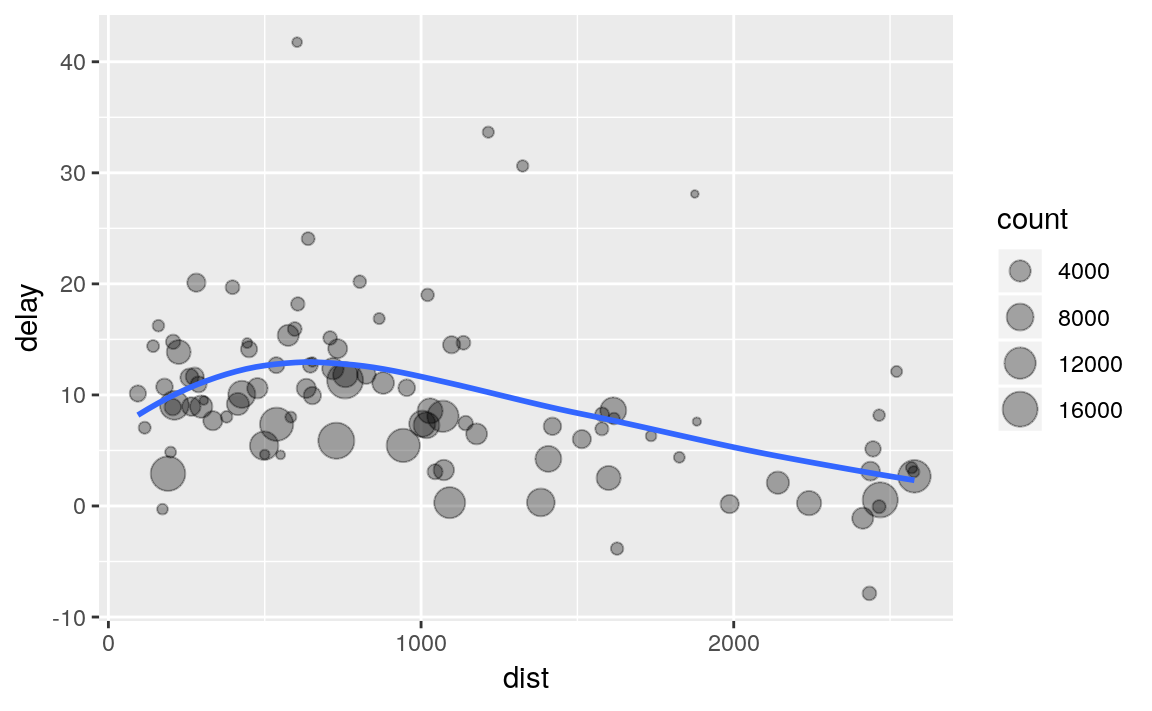
\includegraphics[width=0.7\linewidth]{book_figures/unnamed-chunk-36-1} \end{center}

¡Observa que generamos un gráfico que contiene dos geoms! Si esto te
emociona, abróchate el cinturón. En la siguiente sección aprenderemos
cómo colocar múltiples geoms en el mismo gráfico.

\textbf{ggplot2} proporciona más de 40 geoms y los paquetes de extensión
proporcionan aún más (consulta
\url{https://exts.ggplot2.tidyverse.org/gallery/} para obtener una
muestra). La mejor forma de obtener un panorama completo sobre las
posibilidades que brinda \textbf{ggplot2} es consultando la hoja de
referencia (o \emph{cheatsheet}), que puedes encontrar en
\url{https://rstudio.com/resources/cheatsheets/}. Para obtener más
información sobre un tipo dado de geoms, usa la ayuda:
\texttt{?geom\_smooth}.

Muchos geoms, como \texttt{geom\_smooth()}, usan un único objeto
geométrico para mostrar múltiples filas de datos. Con estos geoms,
puedes asignar la estética de \texttt{group} (\textbf{grupo}) a una
variable categórica para graficar múltiples objetos. \textbf{ggplot2}
representará un objeto distinto por cada valor único de la variable de
agrupamiento. En la práctica, \textbf{ggplot2} agrupará automáticamente
los datos para estos geoms siempre que se asigne una estética a una
variable discreta (como en el ejemplo del tipo de línea o
\texttt{linetype}). Es conveniente confiar en esta característica porque
la estética del grupo en sí misma no agrega una leyenda o
características distintivas a los geoms.

\begin{Shaded}
\begin{Highlighting}[]
\KeywordTok{ggplot}\NormalTok{(}\DataTypeTok{data =}\NormalTok{ millas) }\OperatorTok{+}
\StringTok{  }\KeywordTok{geom_smooth}\NormalTok{(}\DataTypeTok{mapping =} \KeywordTok{aes}\NormalTok{(}\DataTypeTok{x =}\NormalTok{ cilindrada, }\DataTypeTok{y =}\NormalTok{ autopista))}

\KeywordTok{ggplot}\NormalTok{(}\DataTypeTok{data =}\NormalTok{ millas) }\OperatorTok{+}
\StringTok{  }\KeywordTok{geom_smooth}\NormalTok{(}\DataTypeTok{mapping =} \KeywordTok{aes}\NormalTok{(}\DataTypeTok{x =}\NormalTok{ cilindrada, }\DataTypeTok{y =}\NormalTok{ autopista, }\DataTypeTok{group =}\NormalTok{ traccion))}

\KeywordTok{ggplot}\NormalTok{(}\DataTypeTok{data =}\NormalTok{ millas) }\OperatorTok{+}
\StringTok{  }\KeywordTok{geom_smooth}\NormalTok{(}
    \DataTypeTok{mapping =} \KeywordTok{aes}\NormalTok{(}\DataTypeTok{x =}\NormalTok{ cilindrada, }\DataTypeTok{y =}\NormalTok{ autopista, }\DataTypeTok{color =}\NormalTok{ traccion),}
    \DataTypeTok{show.legend =} \OtherTok{FALSE}
\NormalTok{    )}
\end{Highlighting}
\end{Shaded}

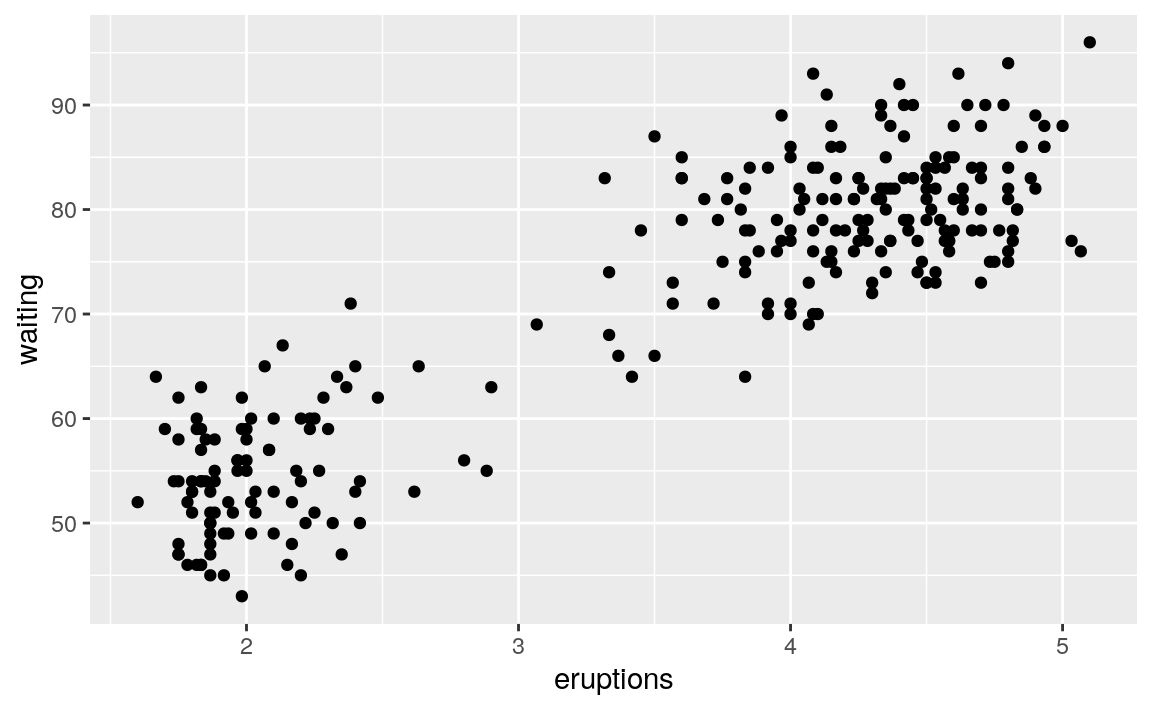
\includegraphics[width=0.33\linewidth]{book_figures/unnamed-chunk-37-1}
\includegraphics[width=0.33\linewidth]{book_figures/unnamed-chunk-37-2}
\includegraphics[width=0.33\linewidth]{book_figures/unnamed-chunk-37-3}

Para mostrar múltiples geoms en el mismo gráfico, agrega varias
funciones geom a \texttt{ggplot()}:

\begin{Shaded}
\begin{Highlighting}[]
\KeywordTok{ggplot}\NormalTok{(}\DataTypeTok{data =}\NormalTok{ millas) }\OperatorTok{+}
\StringTok{ }\KeywordTok{geom_point}\NormalTok{(}\DataTypeTok{mapping =} \KeywordTok{aes}\NormalTok{(}\DataTypeTok{x =}\NormalTok{ cilindrada, }\DataTypeTok{y =}\NormalTok{ autopista)) }\OperatorTok{+}
\StringTok{ }\KeywordTok{geom_smooth}\NormalTok{(}\DataTypeTok{mapping =} \KeywordTok{aes}\NormalTok{(}\DataTypeTok{x =}\NormalTok{ cilindrada, }\DataTypeTok{y =}\NormalTok{ autopista))}
\end{Highlighting}
\end{Shaded}

\begin{center}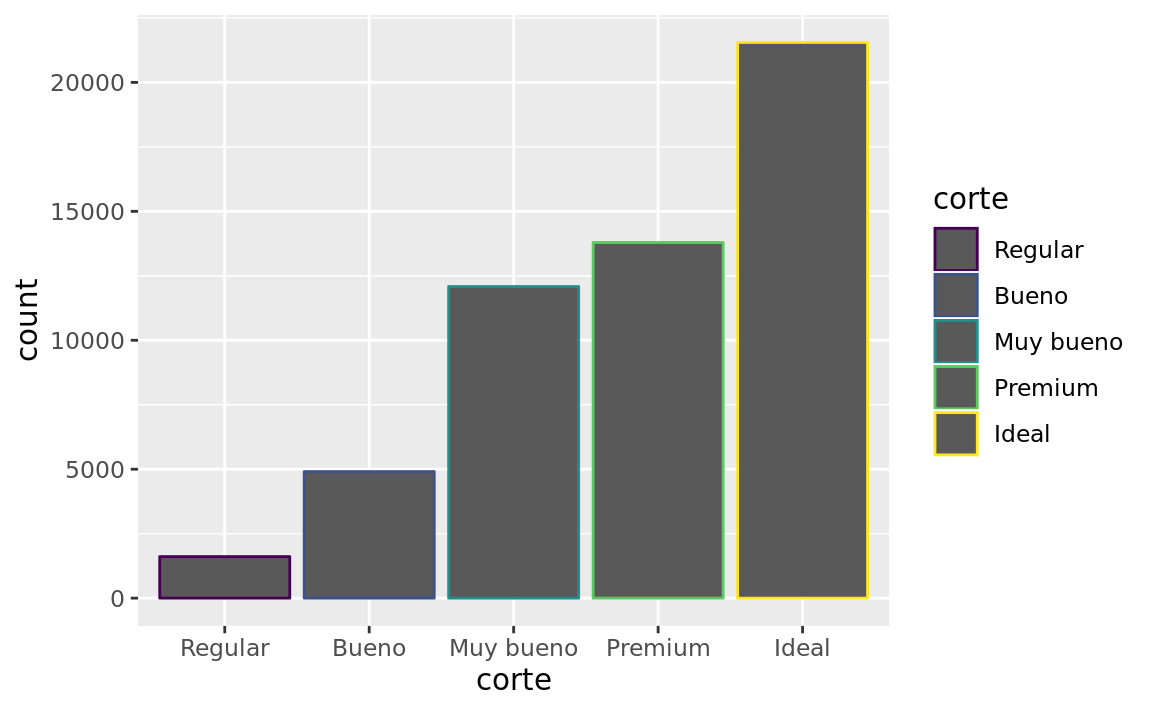
\includegraphics[width=0.7\linewidth]{book_figures/unnamed-chunk-38-1} \end{center}

Esto introduce, sin embargo, cierta duplicación en nuestro código.
Imagina que deseas cambiar el eje y para mostrar \texttt{cilindrada} en
lugar de \texttt{autopista}. Necesitarías cambiar la variable en dos
lugares y podrías olvidarte de actualizar uno. Puedes evitar este tipo
de repetición pasando un conjunto de mapeos a \texttt{ggplot()}.
\textbf{ggplot2} tratará estos mapeos como mapeos globales que se
aplican a cada geom en el gráfico. En otras palabras, este código
producirá la misma gráfica que el código anterior:

\begin{Shaded}
\begin{Highlighting}[]
\KeywordTok{ggplot}\NormalTok{(}\DataTypeTok{data =}\NormalTok{ millas, }\DataTypeTok{mapping =} \KeywordTok{aes}\NormalTok{(}\DataTypeTok{x =}\NormalTok{ cilindrada, }\DataTypeTok{y =}\NormalTok{ autopista)) }\OperatorTok{+}
\StringTok{  }\KeywordTok{geom_point}\NormalTok{() }\OperatorTok{+}
\StringTok{  }\KeywordTok{geom_smooth}\NormalTok{()}
\end{Highlighting}
\end{Shaded}

Si colocas mapeos en una función geom, ggplot2 los tratará como mapeos
locales para la capa. Estas asignaciones serán usadas para extender o
sobrescribir los mapeos globales \emph{solo para esa capa}. Esto permite
mostrar diferentes estéticas en diferentes capas.

\begin{Shaded}
\begin{Highlighting}[]
\KeywordTok{ggplot}\NormalTok{(}\DataTypeTok{data =}\NormalTok{ millas, }\DataTypeTok{mapping =} \KeywordTok{aes}\NormalTok{(}\DataTypeTok{x =}\NormalTok{ cilindrada, }\DataTypeTok{y =}\NormalTok{ autopista)) }\OperatorTok{+}
\StringTok{  }\KeywordTok{geom_point}\NormalTok{(}\DataTypeTok{mapping =} \KeywordTok{aes}\NormalTok{(}\DataTypeTok{color =}\NormalTok{ clase)) }\OperatorTok{+}
\StringTok{  }\KeywordTok{geom_smooth}\NormalTok{()}
\end{Highlighting}
\end{Shaded}

\begin{center}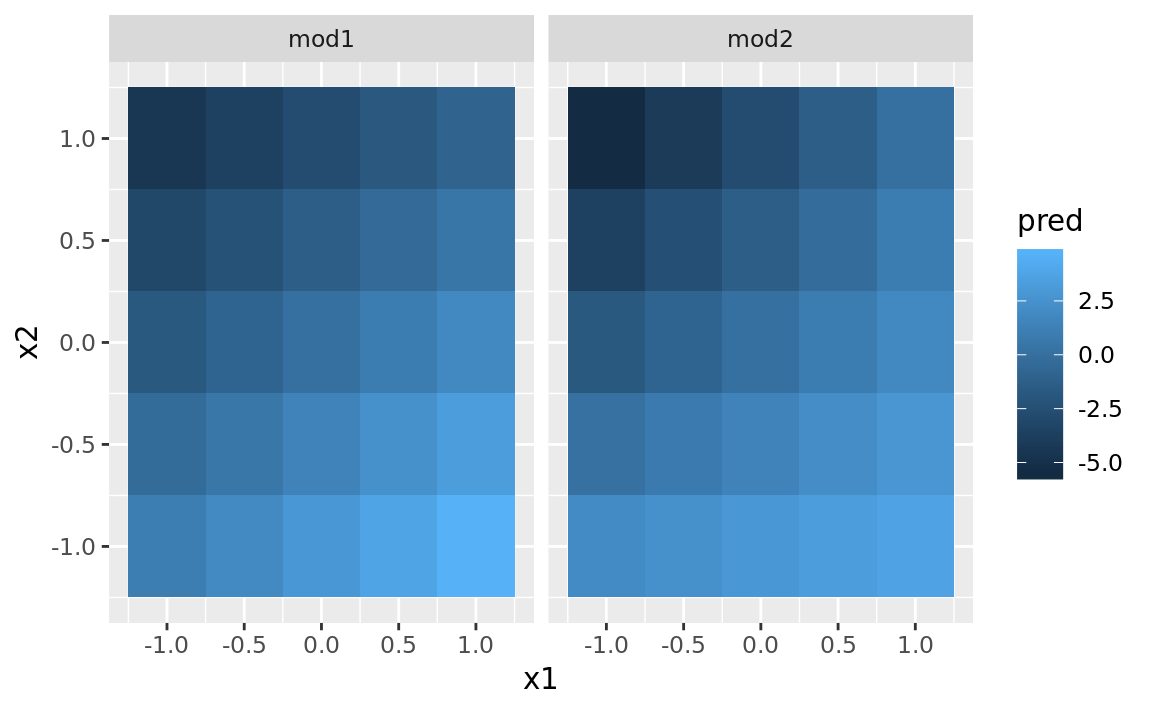
\includegraphics[width=0.7\linewidth]{book_figures/unnamed-chunk-40-1} \end{center}

La misma idea se puede emplear para especificar distintos conjuntos de
datos (\texttt{data}) para cada capa. Aquí, nuestra línea suave muestra
solo un subconjunto del conjunto de datos de \texttt{millas}: los autos
subcompactos. El argumento local de datos en \texttt{geom\_smooth()}
anula el argumento de datos globales en \texttt{ggplot()} solo para esa
capa.

\begin{Shaded}
\begin{Highlighting}[]
\KeywordTok{ggplot}\NormalTok{(}\DataTypeTok{data =}\NormalTok{ millas, }\DataTypeTok{mapping =} \KeywordTok{aes}\NormalTok{(}\DataTypeTok{x =}\NormalTok{ cilindrada, }\DataTypeTok{y =}\NormalTok{ autopista)) }\OperatorTok{+}
\StringTok{  }\KeywordTok{geom_point}\NormalTok{(}\DataTypeTok{mapping =} \KeywordTok{aes}\NormalTok{(}\DataTypeTok{color =}\NormalTok{ clase)) }\OperatorTok{+}
\StringTok{  }\KeywordTok{geom_smooth}\NormalTok{(}\DataTypeTok{data =} \KeywordTok{filter}\NormalTok{(millas, clase }\OperatorTok{==}\StringTok{ "subcompacto"}\NormalTok{), }\DataTypeTok{se =} \OtherTok{FALSE}\NormalTok{)}
\end{Highlighting}
\end{Shaded}

\begin{center}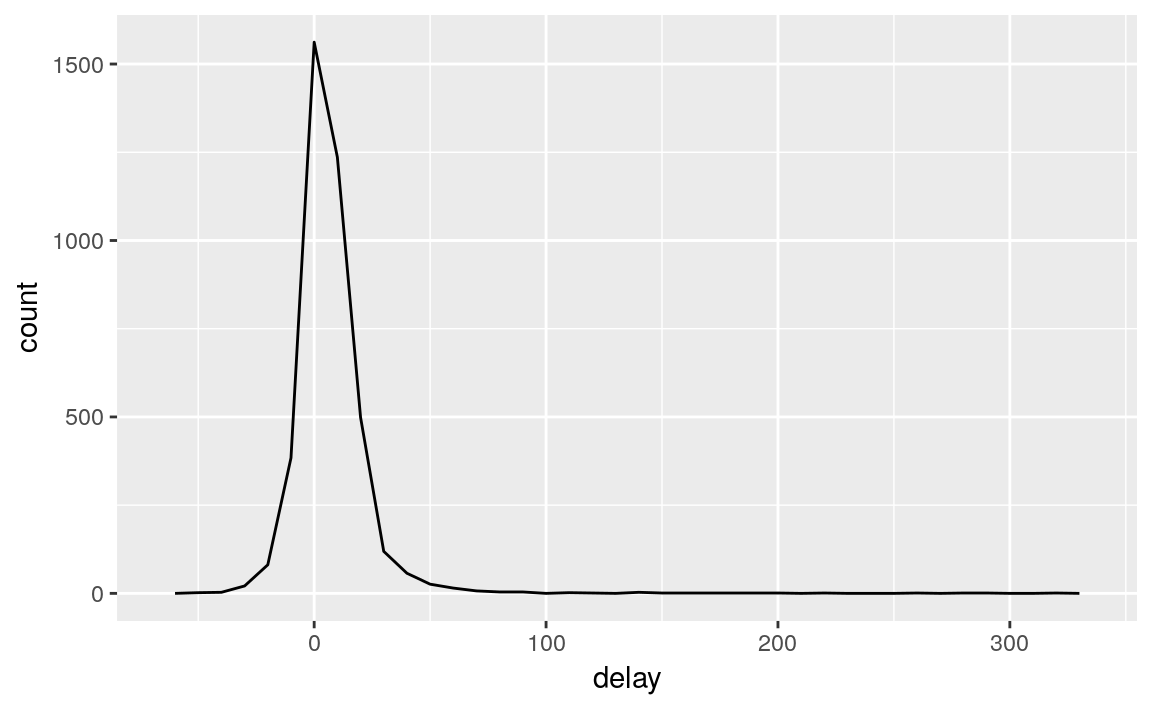
\includegraphics[width=0.7\linewidth]{book_figures/unnamed-chunk-41-1} \end{center}

(Aprenderás cómo funciona \texttt{filter()} en el próximo capítulo: por
ahora, solo recuerda que este comando selecciona los automóviles
subcompactos).

\hypertarget{ejercicios-3}{%
\subsection{Ejercicios}\label{ejercicios-3}}

\begin{enumerate}
\def\labelenumi{\arabic{enumi}.}
\item
  ¿Qué geom usarías para generar un gráfico de líneas? ¿Y para un
  diagrama de caja? ¿Y para un histograma? ¿Y para un gráfico de área?
\item
  Ejecuta este código en tu mente y predice cómo se verá el
  \emph{output}. Luego, ejecuta el código en R y verifica tus
  predicciones.

\begin{Shaded}
\begin{Highlighting}[]
\KeywordTok{ggplot}\NormalTok{(}\DataTypeTok{data =}\NormalTok{ millas, }\DataTypeTok{mapping =} \KeywordTok{aes}\NormalTok{(}\DataTypeTok{x =}\NormalTok{ cilindrada, }\DataTypeTok{y =}\NormalTok{ autopista, }\DataTypeTok{color =}\NormalTok{ traccion)) }\OperatorTok{+}
\StringTok{  }\KeywordTok{geom_point}\NormalTok{() }\OperatorTok{+}
\StringTok{  }\KeywordTok{geom_smooth}\NormalTok{(}\DataTypeTok{se =} \OtherTok{FALSE}\NormalTok{)}
\end{Highlighting}
\end{Shaded}
\item
  ¿Qué muestra \texttt{show.legend\ =\ FALSE}? ¿Qué pasa si lo quitas?
  ¿Por qué crees que lo utilizamos antes en el capítulo?
\item
  ¿Qué hace el argumento \texttt{se} en \texttt{geom\_smooth()}?
\item
  ¿Se verán distintos estos gráficos? ¿Por qué sí o por qué no?

\begin{Shaded}
\begin{Highlighting}[]
\KeywordTok{ggplot}\NormalTok{(}\DataTypeTok{data =}\NormalTok{ millas, }\DataTypeTok{mapping =} \KeywordTok{aes}\NormalTok{(}\DataTypeTok{x =}\NormalTok{ cilindrada, }\DataTypeTok{y =}\NormalTok{ autopista)) }\OperatorTok{+}
\StringTok{  }\KeywordTok{geom_point}\NormalTok{() }\OperatorTok{+}
\StringTok{  }\KeywordTok{geom_smooth}\NormalTok{()}

\KeywordTok{ggplot}\NormalTok{() }\OperatorTok{+}
\StringTok{  }\KeywordTok{geom_point}\NormalTok{(}\DataTypeTok{data =}\NormalTok{ millas, }\DataTypeTok{mapping =} \KeywordTok{aes}\NormalTok{(}\DataTypeTok{x =}\NormalTok{ cilindrada, }\DataTypeTok{y =}\NormalTok{ autopista)) }\OperatorTok{+}
\StringTok{  }\KeywordTok{geom_smooth}\NormalTok{(}\DataTypeTok{data =}\NormalTok{ millas, }\DataTypeTok{mapping =} \KeywordTok{aes}\NormalTok{(}\DataTypeTok{x =}\NormalTok{ cilindrada, }\DataTypeTok{y =}\NormalTok{ autopista))}
\end{Highlighting}
\end{Shaded}
\item
  Recrea el código R necesario para generar los siguientes gráficos:

  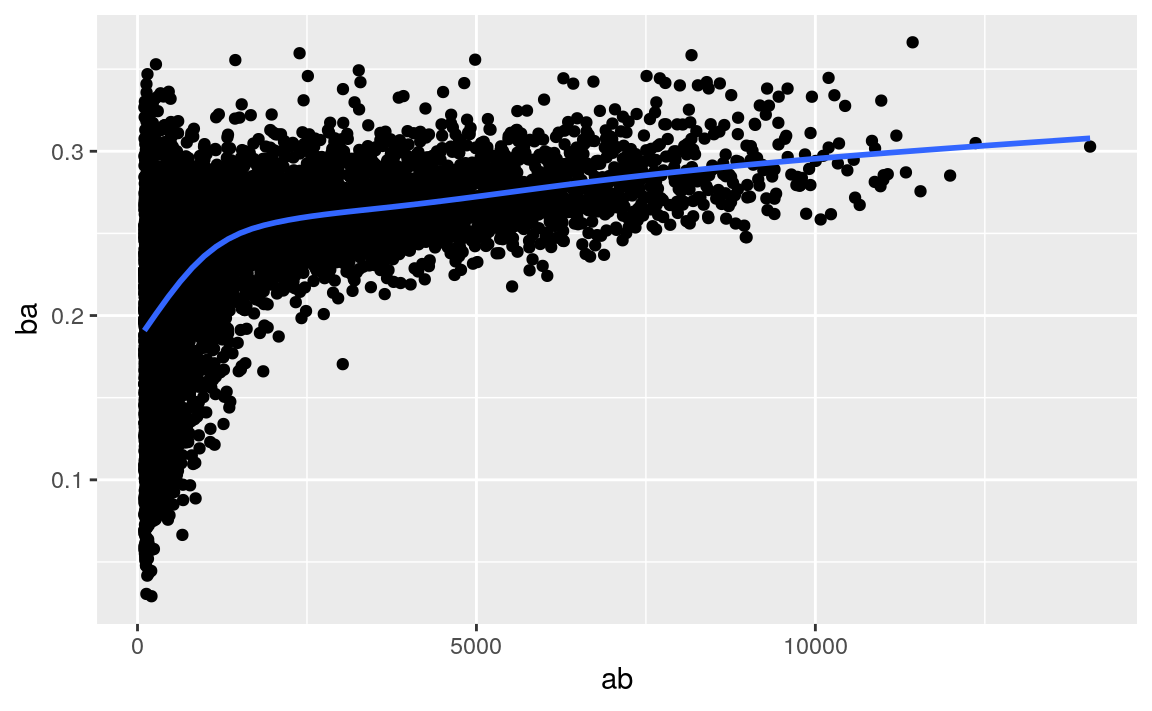
\includegraphics[width=0.5\linewidth]{book_figures/unnamed-chunk-44-1}
  \includegraphics[width=0.5\linewidth]{book_figures/unnamed-chunk-44-2}
  \includegraphics[width=0.5\linewidth]{book_figures/unnamed-chunk-44-3}
  \includegraphics[width=0.5\linewidth]{book_figures/unnamed-chunk-44-4}
  \includegraphics[width=0.5\linewidth]{book_figures/unnamed-chunk-44-5}
  \includegraphics[width=0.5\linewidth]{book_figures/unnamed-chunk-44-6}
\end{enumerate}

\hypertarget{transformaciones-estaduxedsticas}{%
\section{Transformaciones
estadísticas}\label{transformaciones-estaduxedsticas}}

A continuación, echemos un vistazo a un gráfico de barras. Los gráficos
de barras parecen simples, pero son interesantes porque revelan algo
sutil sobre los gráficos. Considera un gráfico de barras básico, como
uno realizado con \texttt{geom\_bar()}. El siguiente gráfico muestra la
cantidad total de diamantes en el conjunto de datos \texttt{diamantes},
agrupados por la variable \texttt{corte}. El conjunto de datos
\texttt{diamantes} se encuentra en el paquete \textbf{datos} y contiene
información sobre \textasciitilde{} 54000 diamantes, incluido el
\texttt{precio}, el \texttt{quilate}, el \texttt{color}, la
\texttt{claridad} y el \texttt{corte} de cada uno. El gráfico muestra
que hay más diamantes disponibles con cortes de alta calidad que con
cortes de baja calidad.

\begin{Shaded}
\begin{Highlighting}[]
\KeywordTok{ggplot}\NormalTok{(}\DataTypeTok{data =}\NormalTok{ diamantes) }\OperatorTok{+}
\StringTok{  }\KeywordTok{geom_bar}\NormalTok{(}\DataTypeTok{mapping =} \KeywordTok{aes}\NormalTok{(}\DataTypeTok{x =}\NormalTok{ corte))}
\end{Highlighting}
\end{Shaded}

\begin{center}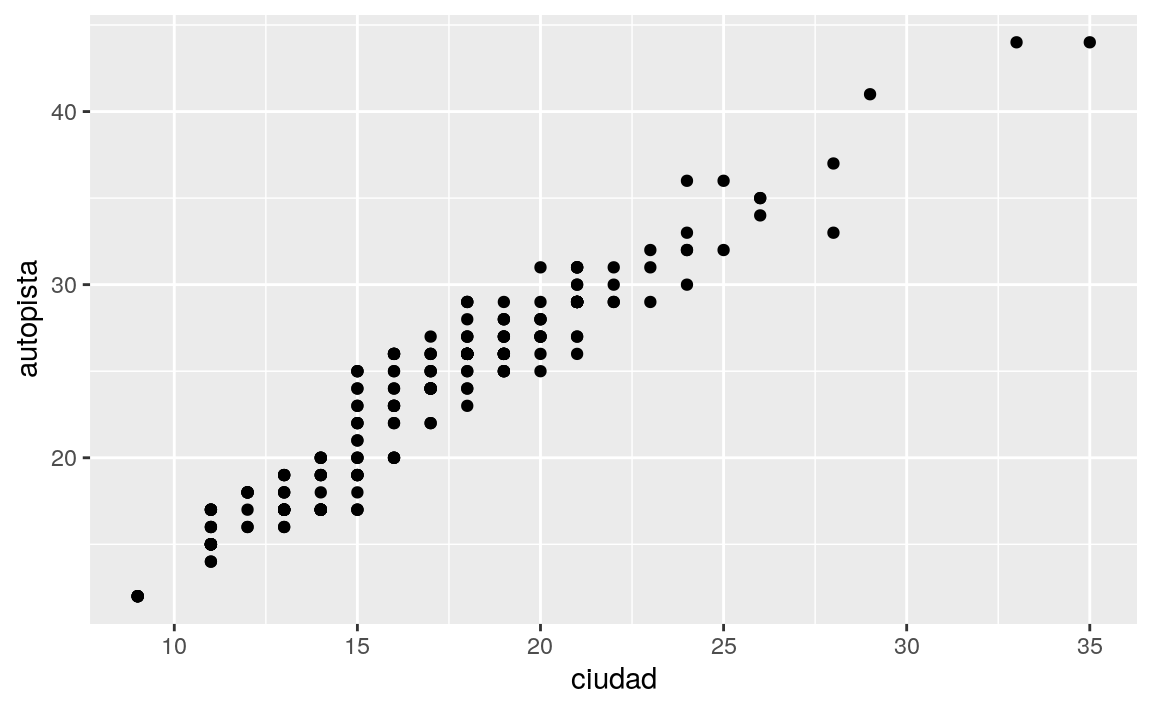
\includegraphics[width=0.7\linewidth]{book_figures/unnamed-chunk-45-1} \end{center}

En el eje x, el gráfico muestra \texttt{corte}, una variable de
\texttt{diamantes}. En el eje y muestra `recuento' (\emph{count}), ¡pero
el recuento no es una variable en \texttt{diamantes}! ¿De dónde viene?
Muchos gráficos, como los diagramas de dispersión (\emph{scatterplots}),
grafican los valores brutos de un conjunto de datos. Otros gráficos,
como los de barras, calculan nuevos valores para presentar:

\begin{itemize}
\item
  los gráficos de barras, los histogramas y los polígonos de frecuencia
  almacenan los datos y luego grafican los conteos por contenedores, es
  decir, el número de puntos que caen en cada contenedor.
\item
  los gráficos de líneas suavizadas (\emph{smoothers}) ajustan un modelo
  a los datos y luego grafican las predicciones del modelo.
\item
  los diagramas de caja (\emph{boxplots}) calculan un resumen robusto de
  la distribución y luego muestran una caja con formato especial.
\end{itemize}

El algoritmo utilizado para calcular nuevos valores para un gráfico se
llama \emph{stat}, abreviatura en inglés de transformación estadística
(\emph{\textbf{stat}tistical transformation}). La siguiente figura
describe cómo funciona este proceso con \texttt{geom\_bar()}.

\begin{center}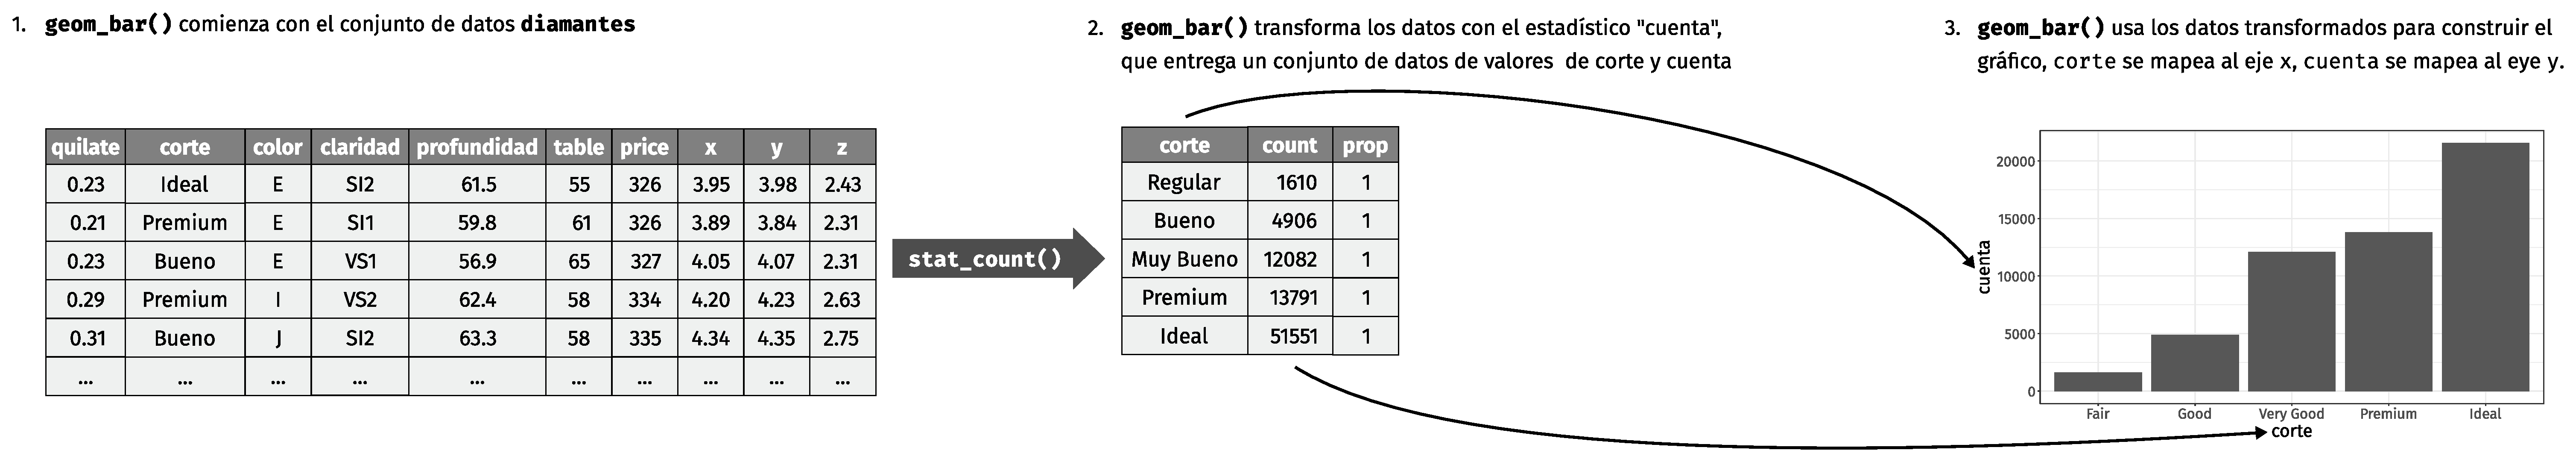
\includegraphics[width=1\linewidth]{diagrams_pdf/es/visualization-stat-bar} \end{center}

Puedes aprender acerca de qué \emph{stat} usa cada geom inspeccionando
el valor predeterminado para el argumento \texttt{stat}. Por ejemplo,
\texttt{?geom\_bar} muestra que el valor predeterminado para
\texttt{stat} es ``count'', lo que significa que \texttt{geom\_bar()}
usa \texttt{stat\_count()}. \texttt{stat\_count()} está documentado en
la misma página que \texttt{geom\_bar()}, y si te desplazas hacia abajo
puedes encontrar una sección llamada ``Computed variables''
(\emph{Variables calculadas}). Ahí se describe cómo calcula dos nuevas
variables: \texttt{count} y \texttt{prop}.

Por lo general, puedes usar geoms y estadísticas de forma
intercambiable. Por ejemplo, puedes volver a crear la gráfica anterior
usando \texttt{stat\_count()} en lugar de \texttt{geom\_bar()}:

\begin{Shaded}
\begin{Highlighting}[]
\KeywordTok{ggplot}\NormalTok{(}\DataTypeTok{data =}\NormalTok{ diamantes) }\OperatorTok{+}
\StringTok{  }\KeywordTok{stat_count}\NormalTok{(}\DataTypeTok{mapping =} \KeywordTok{aes}\NormalTok{(}\DataTypeTok{x =}\NormalTok{ corte))}
\end{Highlighting}
\end{Shaded}

\begin{center}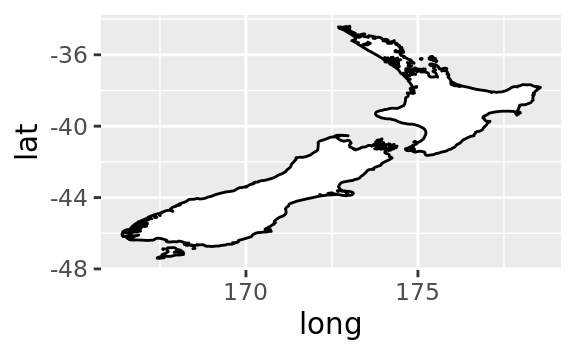
\includegraphics[width=0.7\linewidth]{book_figures/unnamed-chunk-47-1} \end{center}

Esto funciona porque cada geom tiene una estadística predeterminada, y
cada estadística tiene un geom predeterminado. Esto significa que
generalmente puedes usar geoms sin preocuparte por la transformación
estadística subyacente.

Hay tres razones por las que podrías necesitar usar una estadística
explícitamente:

\begin{enumerate}
\def\labelenumi{\arabic{enumi}.}
\item
  Es posible que desees anular la estadística predeterminada. En el
  siguiente código, cambiamos en \texttt{geom\_bar()} la estadística
  recuento (``count'', el valor predeterminado) a identidad
  (``identity''). Esto nos permite asignar la altura de las barras a los
  valores brutos de una variable \(y\). Desafortunadamente, cuando las
  personas hablan de gráficos de barras de manera informal, podrían
  estar refiriéndose a este tipo de gráfico de barras, en el que la
  altura de la barra ya está presente en los datos, o bien, al gráfico
  de barras anterior, en el que la altura de la barra se determina
  contando filas.

\begin{Shaded}
\begin{Highlighting}[]
\NormalTok{demo <-}\StringTok{ }\KeywordTok{tribble}\NormalTok{(}
  \OperatorTok{~}\NormalTok{corte,     }\OperatorTok{~}\NormalTok{freq,}
  \StringTok{"Regular"}\NormalTok{,   }\DecValTok{1610}\NormalTok{,}
  \StringTok{"Bueno"}\NormalTok{,     }\DecValTok{4906}\NormalTok{,}
  \StringTok{"Muy Bueno"}\NormalTok{, }\DecValTok{12082}\NormalTok{,}
  \StringTok{"Premium"}\NormalTok{,   }\DecValTok{13791}\NormalTok{,}
  \StringTok{"Ideal"}\NormalTok{,     }\DecValTok{21551}
\NormalTok{)}

\KeywordTok{ggplot}\NormalTok{(}\DataTypeTok{data =}\NormalTok{ demo) }\OperatorTok{+}
\StringTok{  }\KeywordTok{geom_bar}\NormalTok{(}\DataTypeTok{mapping =} \KeywordTok{aes}\NormalTok{(}\DataTypeTok{x =}\NormalTok{ corte, }\DataTypeTok{y =}\NormalTok{ freq), }\DataTypeTok{stat =} \StringTok{"identity"}\NormalTok{)}
\end{Highlighting}
\end{Shaded}

  \begin{center}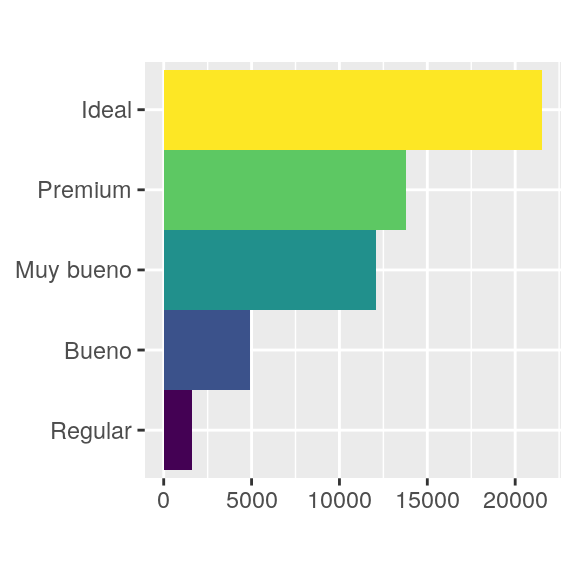
\includegraphics[width=0.7\linewidth]{book_figures/unnamed-chunk-48-1} \end{center}

  (No te preocupes si nunca has visto \texttt{\textless{}-} o
  \texttt{tribble()}. Puede que seas capaz de adivinar su significado
  por el contexto y ¡pronto aprenderás qué es lo que hacen exactamente!)
\item
  Es posible que desees anular el mapeo predeterminado de las variables
  transformadas a las estéticas. Por ejemplo, es posible que desees
  mostrar un gráfico de barras de proporciones, en lugar de un recuento:

\begin{Shaded}
\begin{Highlighting}[]
\KeywordTok{ggplot}\NormalTok{(}\DataTypeTok{data =}\NormalTok{ diamantes) }\OperatorTok{+}
\StringTok{  }\KeywordTok{geom_bar}\NormalTok{(}\DataTypeTok{mapping =} \KeywordTok{aes}\NormalTok{(}\DataTypeTok{x =}\NormalTok{ corte, }\DataTypeTok{y =} \KeywordTok{stat}\NormalTok{(prop), }\DataTypeTok{group =} \DecValTok{1}\NormalTok{))}
\end{Highlighting}
\end{Shaded}

  \begin{center}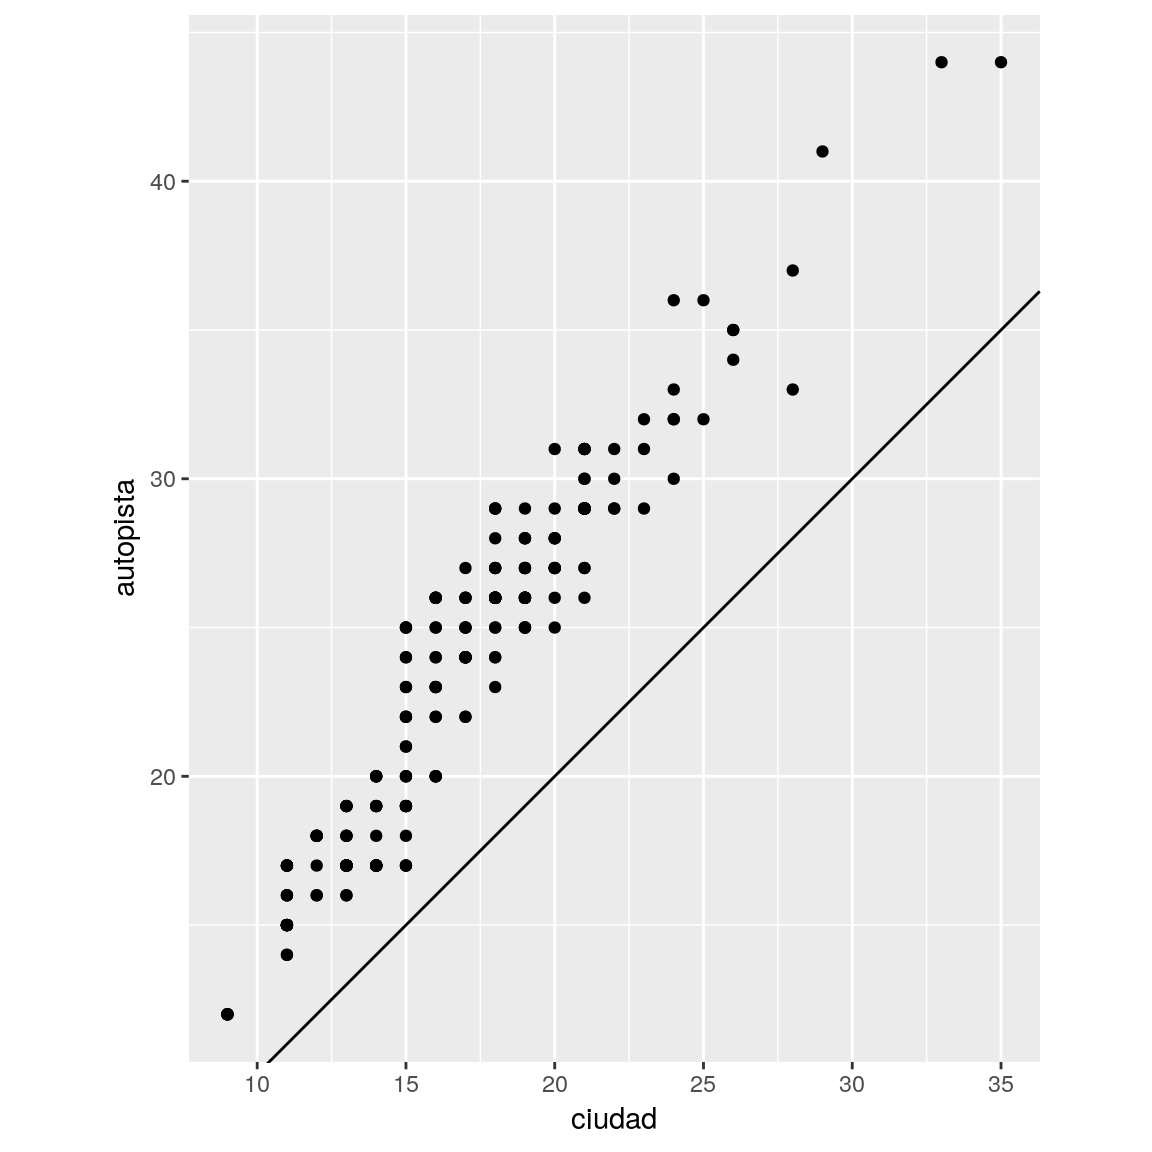
\includegraphics[width=0.7\linewidth]{book_figures/unnamed-chunk-49-1} \end{center}

  Para encontrar las variables calculadas por \emph{stat}, busca la
  sección de ayuda titulada ``Compute Variables''.
\item
  Es posible que desees resaltar la transformación estadística en tu
  código. Por ejemplo, puedes usar \texttt{stat\_summary()}, que resume
  los valores de y para cada valor único de x, para así resaltar el
  resumen que se está computando:

\begin{Shaded}
\begin{Highlighting}[]
\KeywordTok{ggplot}\NormalTok{(}\DataTypeTok{data =}\NormalTok{ diamantes) }\OperatorTok{+}
\StringTok{  }\KeywordTok{stat_summary}\NormalTok{(}
    \DataTypeTok{mapping =} \KeywordTok{aes}\NormalTok{(}\DataTypeTok{x =}\NormalTok{ corte, }\DataTypeTok{y =}\NormalTok{ profundidad),}
    \DataTypeTok{fun.min =}\NormalTok{ min,}
    \DataTypeTok{fun.max =}\NormalTok{ max,}
    \DataTypeTok{fun =}\NormalTok{ median}
\NormalTok{  )}
\end{Highlighting}
\end{Shaded}

  \begin{center}\includegraphics[width=0.7\linewidth]{book_figures/unnamed-chunk-50-1} \end{center}
\end{enumerate}

\textbf{ggplot2} proporciona más de 20 transformaciones estadísticas
para que uses. Cada \emph{stat} es una función, por lo que puedes
obtener ayuda de la manera habitual, por ejemplo: \texttt{?stat\_bin}.
Para ver una lista completa de transformaciones estadísticas disponibles
para \textbf{ggplot2}, consulta la hoja de referencia.

\hypertarget{ejercicios-4}{%
\subsection{Ejercicios}\label{ejercicios-4}}

\begin{enumerate}
\def\labelenumi{\arabic{enumi}.}
\item
  ¿Cuál es el geom predeterminado asociado con \texttt{stat\_summary()}?
  ¿Cómo podrías reescribir el gráfico anterior para usar esa función
  geom en lugar de la función stat?
\item
  ¿Qué hace \texttt{geom\_col()}? ¿En qué se diferencia de
  \texttt{geom\_bar()}?
\item
  La mayoría de los geoms y las transformaciones estadísticas vienen en
  pares que casi siempre se usan en conjunto. Lee la documentación y haz
  una lista de todos los pares. ¿Qué tienen en común?
\item
  ¿Qué variables calcula \texttt{stat\_smooth()}? ¿Qué parámetros
  controlan su comportamiento?
\item
  En nuestro gráfico de barras de proporción necesitamos establecer
  \texttt{group\ =\ 1}. ¿Por qué? En otras palabras, ¿cuál es el
  problema con estos dos gráficos?

\begin{Shaded}
\begin{Highlighting}[]
\KeywordTok{ggplot}\NormalTok{(}\DataTypeTok{data =}\NormalTok{ diamantes) }\OperatorTok{+}
\StringTok{  }\KeywordTok{geom_bar}\NormalTok{(}\DataTypeTok{mapping =} \KeywordTok{aes}\NormalTok{(}\DataTypeTok{x =}\NormalTok{ corte, }\DataTypeTok{y =}\NormalTok{ ..prop..))}

\KeywordTok{ggplot}\NormalTok{(}\DataTypeTok{data =}\NormalTok{ diamantes) }\OperatorTok{+}
\StringTok{  }\KeywordTok{geom_bar}\NormalTok{(}\DataTypeTok{mapping =} \KeywordTok{aes}\NormalTok{(}\DataTypeTok{x =}\NormalTok{ corte, }\DataTypeTok{fill =}\NormalTok{ color, }\DataTypeTok{y =}\NormalTok{ ..prop..))}
\end{Highlighting}
\end{Shaded}
\end{enumerate}

\hypertarget{ajustes-de-posiciuxf3n}{%
\section{Ajustes de posición}\label{ajustes-de-posiciuxf3n}}

Hay una pieza más de magia asociada con los gráficos de barras. Puedes
colorear un gráfico de barras usando tanto la estética de \texttt{color}
como la más útil \texttt{fill} (\emph{relleno}):

\begin{Shaded}
\begin{Highlighting}[]
\KeywordTok{ggplot}\NormalTok{(}\DataTypeTok{data =}\NormalTok{ diamantes) }\OperatorTok{+}
\StringTok{  }\KeywordTok{geom_bar}\NormalTok{(}\DataTypeTok{mapping =} \KeywordTok{aes}\NormalTok{(}\DataTypeTok{x =}\NormalTok{ corte, }\DataTypeTok{colour =}\NormalTok{ corte))}

\KeywordTok{ggplot}\NormalTok{(}\DataTypeTok{data =}\NormalTok{ diamantes) }\OperatorTok{+}
\StringTok{  }\KeywordTok{geom_bar}\NormalTok{(}\DataTypeTok{mapping =} \KeywordTok{aes}\NormalTok{(}\DataTypeTok{x =}\NormalTok{ corte, }\DataTypeTok{fill =}\NormalTok{ corte))}
\end{Highlighting}
\end{Shaded}

\includegraphics[width=0.5\linewidth]{book_figures/unnamed-chunk-52-1}
\includegraphics[width=0.5\linewidth]{book_figures/unnamed-chunk-52-2}

Mira lo que sucede si asignas la estética de relleno (\emph{fill}) a
otra variable, como \texttt{claridad}: las barras se apilan
automáticamente. Cada rectángulo de color representa una combinación de
\texttt{corte} y \texttt{claridad}.

\begin{Shaded}
\begin{Highlighting}[]
\KeywordTok{ggplot}\NormalTok{(}\DataTypeTok{data =}\NormalTok{ diamantes) }\OperatorTok{+}
\StringTok{  }\KeywordTok{geom_bar}\NormalTok{(}\DataTypeTok{mapping =} \KeywordTok{aes}\NormalTok{(}\DataTypeTok{x =}\NormalTok{ corte, }\DataTypeTok{fill =}\NormalTok{ claridad))}
\end{Highlighting}
\end{Shaded}

\begin{center}\includegraphics[width=0.7\linewidth]{book_figures/unnamed-chunk-53-1} \end{center}

El apilamiento se realiza automáticamente mediante el ajuste de posición
especificado por el argumento \texttt{position}. Si no deseas un gráfico
de barras apiladas (\texttt{"stack"}), puedes usar una de las otras tres
opciones: \texttt{"identity"}, \texttt{"dodge"} o \texttt{"fill"}.

\begin{itemize}
\item
  \texttt{position\ =\ "identity"} colocará cada objeto exactamente
  donde cae en el contexto del gráfico. Esto no es muy útil al momento
  de graficar barras, ya que las superpone. Para ver esa superposición,
  debemos hacer que las barras sean ligeramente transparentes
  configurando el \texttt{alpha} a un valor pequeño, o completamente
  transparente al establecer \texttt{fill\ =\ NA}.

\begin{Shaded}
\begin{Highlighting}[]
\KeywordTok{ggplot}\NormalTok{(}\DataTypeTok{data =}\NormalTok{ diamantes, }\DataTypeTok{mapping =} \KeywordTok{aes}\NormalTok{(}\DataTypeTok{x =}\NormalTok{ corte, }\DataTypeTok{fill =}\NormalTok{ claridad)) }\OperatorTok{+}
\StringTok{  }\KeywordTok{geom_bar}\NormalTok{(}\DataTypeTok{alpha =} \DecValTok{1}\OperatorTok{/}\DecValTok{5}\NormalTok{, }\DataTypeTok{position =} \StringTok{"identity"}\NormalTok{)}

\KeywordTok{ggplot}\NormalTok{(}\DataTypeTok{data =}\NormalTok{ diamantes, }\DataTypeTok{mapping =} \KeywordTok{aes}\NormalTok{(}\DataTypeTok{x =}\NormalTok{ corte, }\DataTypeTok{colour =}\NormalTok{ claridad)) }\OperatorTok{+}
\StringTok{  }\KeywordTok{geom_bar}\NormalTok{(}\DataTypeTok{fill =} \OtherTok{NA}\NormalTok{, }\DataTypeTok{position =} \StringTok{"identity"}\NormalTok{)}
\end{Highlighting}
\end{Shaded}

  \includegraphics[width=0.5\linewidth]{book_figures/unnamed-chunk-54-1}
  \includegraphics[width=0.5\linewidth]{book_figures/unnamed-chunk-54-2}
\end{itemize}

El ajuste de \texttt{position\ =\ identity} es más útil para geoms 2D,
como puntos, donde es la opción predeterminada.

\begin{itemize}
\item
  \texttt{position\ =\ "fill"} funciona como el apilamiento de
  \texttt{position\ =\ "stack"}, pero hace que cada conjunto de barras
  apiladas tenga la misma altura. Esto hace que sea más fácil comparar
  proporciones entre grupos.

\begin{Shaded}
\begin{Highlighting}[]
\KeywordTok{ggplot}\NormalTok{(}\DataTypeTok{data =}\NormalTok{ diamantes) }\OperatorTok{+}
\StringTok{  }\KeywordTok{geom_bar}\NormalTok{(}\DataTypeTok{mapping =} \KeywordTok{aes}\NormalTok{(}\DataTypeTok{x =}\NormalTok{ corte, }\DataTypeTok{fill =}\NormalTok{ claridad), }\DataTypeTok{position =} \StringTok{"fill"}\NormalTok{)}
\end{Highlighting}
\end{Shaded}

  \begin{center}\includegraphics[width=0.7\linewidth]{book_figures/unnamed-chunk-55-1} \end{center}
\item
  \texttt{position\ =\ "dodge"} coloca los objetos superpuestos uno al
  lado del otro. Esto hace que sea más fácil comparar valores
  individuales.

\begin{Shaded}
\begin{Highlighting}[]
\KeywordTok{ggplot}\NormalTok{(}\DataTypeTok{data =}\NormalTok{ diamantes) }\OperatorTok{+}
\StringTok{  }\KeywordTok{geom_bar}\NormalTok{(}\DataTypeTok{mapping =} \KeywordTok{aes}\NormalTok{(}\DataTypeTok{x =}\NormalTok{ corte, }\DataTypeTok{fill =}\NormalTok{ claridad), }\DataTypeTok{position =} \StringTok{"dodge"}\NormalTok{)}
\end{Highlighting}
\end{Shaded}

  \begin{center}\includegraphics[width=0.7\linewidth]{book_figures/unnamed-chunk-56-1} \end{center}
\end{itemize}

Hay otro tipo de ajuste que no es útil para gráficos de barras, pero que
puede ser muy útil para diagramas de dispersión. Recuerda nuestro primer
diagrama de dispersión. ¿Notaste que mostraba solo 126 puntos, a pesar
de que hay 234 observaciones en el conjunto de datos?

\begin{center}\includegraphics[width=0.7\linewidth]{book_figures/unnamed-chunk-57-1} \end{center}

Los valores de las variables \texttt{autopista} y \texttt{cilindrada} se
redondean de modo que los puntos aparecen en una cuadrícula y muchos se
superponen entre sí. Este problema se conoce como \textbf{solapamiento}
(\emph{overplotting}). Esta disposición hace que sea difícil ver dónde
está la masa de datos. ¿Los puntos de datos se distribuyen
equitativamente a lo largo de la gráfica, o hay una combinación especial
de \texttt{autopista} y \texttt{cilindrada} que contiene 109 valores?

Puedes evitar esto estableciendo el ajuste de posición en ``jitter''.
\texttt{position\ =\ "jitter"} agrega una pequeña cantidad de ruido
aleatorio a cada punto. Esto dispersa los puntos, ya que es poco
probable que dos puntos reciban la misma cantidad de ruido aleatorio.

\begin{Shaded}
\begin{Highlighting}[]
\KeywordTok{ggplot}\NormalTok{(}\DataTypeTok{data =}\NormalTok{ millas) }\OperatorTok{+}
\StringTok{  }\KeywordTok{geom_point}\NormalTok{(}\DataTypeTok{mapping =} \KeywordTok{aes}\NormalTok{(}\DataTypeTok{x =}\NormalTok{ cilindrada, }\DataTypeTok{y =}\NormalTok{ autopista), }\DataTypeTok{position =} \StringTok{"jitter"}\NormalTok{)}
\end{Highlighting}
\end{Shaded}

\begin{center}\includegraphics[width=0.7\linewidth]{book_figures/unnamed-chunk-58-1} \end{center}

Agregar aleatoriedad a los puntos puede parecer una forma extraña de
mejorar tu gráfico. Si bien hace que sea menos preciso a escalas
pequeñas, lo hace ser más revelador a gran escala. Como esta es una
operación tan útil, ggplot2 incluye una abreviatura de
\texttt{geom\_point(position\ =\ "jitter")}: \texttt{geom\_jitter()}.

Para obtener más información sobre ajustes de posición, busca la página
de ayuda asociada con cada ajuste: \texttt{?position\_dodge},
\texttt{?position\_fill}, \texttt{?position\_identity},
\texttt{?position\_jitter} y \texttt{?position\_stack}.

\hypertarget{ejercicios-5}{%
\subsection{Ejercicios}\label{ejercicios-5}}

\begin{enumerate}
\def\labelenumi{\arabic{enumi}.}
\item
  ¿Cuál es el problema con este gráfico? ¿Cómo podrías mejorarlo?

\begin{Shaded}
\begin{Highlighting}[]
\KeywordTok{ggplot}\NormalTok{(}\DataTypeTok{data =}\NormalTok{ millas, }\DataTypeTok{mapping =} \KeywordTok{aes}\NormalTok{(}\DataTypeTok{x =}\NormalTok{ ciudad, }\DataTypeTok{y =}\NormalTok{ autopista)) }\OperatorTok{+}
\StringTok{  }\KeywordTok{geom_point}\NormalTok{()}
\end{Highlighting}
\end{Shaded}

  \begin{center}\includegraphics[width=0.7\linewidth]{book_figures/unnamed-chunk-59-1} \end{center}
\item
  ¿Qué parámetros de \texttt{geom\_jitter()} controlan la cantidad de
  ruido?
\item
  Compara y contrasta \texttt{geom\_jitter()} con \texttt{geom\_count()}
\item
  ¿Cuál es el ajuste de posición predeterminado de
  \texttt{geom\_boxplot()}? Crea una visualización del conjunto de datos
  de \texttt{millas} que lo demuestre.
\end{enumerate}

\hypertarget{sistemas-de-coordenadas}{%
\section{Sistemas de coordenadas}\label{sistemas-de-coordenadas}}

Los sistemas de coordenadas son probablemente la parte más complicada de
ggplot2. El sistema predeterminado es el sistema de coordenadas
cartesianas, donde las posiciones x e y actúan independientemente para
determinar la ubicación de cada punto. Hay varios otros sistemas de
coordenadas que ocasionalmente son útiles.

\begin{itemize}
\item
  \texttt{coord\_flip()} cambia los ejes x e y. Esto es útil, por
  ejemplo, si quieres diagramas de caja horizontales. También es útil
  para etiquetas largas: es difícil ajustarlas sin que se superpongan en
  el eje x.

\begin{Shaded}
\begin{Highlighting}[]
\KeywordTok{ggplot}\NormalTok{(}\DataTypeTok{data =}\NormalTok{ millas, }\DataTypeTok{mapping =} \KeywordTok{aes}\NormalTok{(}\DataTypeTok{x =}\NormalTok{ clase, }\DataTypeTok{y =}\NormalTok{ autopista)) }\OperatorTok{+}
\StringTok{  }\KeywordTok{geom_boxplot}\NormalTok{()}

\KeywordTok{ggplot}\NormalTok{(}\DataTypeTok{data =}\NormalTok{ millas, }\DataTypeTok{mapping =} \KeywordTok{aes}\NormalTok{(}\DataTypeTok{x =}\NormalTok{ clase, }\DataTypeTok{y =}\NormalTok{ autopista)) }\OperatorTok{+}
\StringTok{  }\KeywordTok{geom_boxplot}\NormalTok{() }\OperatorTok{+}
\StringTok{  }\KeywordTok{coord_flip}\NormalTok{()}
\end{Highlighting}
\end{Shaded}

  \includegraphics[width=0.5\linewidth]{book_figures/unnamed-chunk-60-1}
  \includegraphics[width=0.5\linewidth]{book_figures/unnamed-chunk-60-2}
\item
  \texttt{coord\_quickmap()} establece correctamente la relación de
  aspecto para los mapas. Esto es muy importante si gráficas datos
  espaciales con ggplot2 (tema para el que, desafortunadamente, no
  contamos con espacio para desarrollar en este libro).

\begin{Shaded}
\begin{Highlighting}[]
\NormalTok{nz <-}\StringTok{ }\KeywordTok{map_data}\NormalTok{(}\StringTok{"nz"}\NormalTok{)}

\KeywordTok{ggplot}\NormalTok{(nz, }\KeywordTok{aes}\NormalTok{(long, lat, }\DataTypeTok{group =}\NormalTok{ group)) }\OperatorTok{+}
\StringTok{  }\KeywordTok{geom_polygon}\NormalTok{(}\DataTypeTok{fill =} \StringTok{"white"}\NormalTok{, }\DataTypeTok{colour =} \StringTok{"black"}\NormalTok{)}

\KeywordTok{ggplot}\NormalTok{(nz, }\KeywordTok{aes}\NormalTok{(long, lat, }\DataTypeTok{group =}\NormalTok{ group)) }\OperatorTok{+}
\StringTok{  }\KeywordTok{geom_polygon}\NormalTok{(}\DataTypeTok{fill =} \StringTok{"white"}\NormalTok{, }\DataTypeTok{colour =} \StringTok{"black"}\NormalTok{) }\OperatorTok{+}
\StringTok{  }\KeywordTok{coord_quickmap}\NormalTok{()}
\end{Highlighting}
\end{Shaded}

  \includegraphics[width=0.5\linewidth]{book_figures/unnamed-chunk-61-1}
  \includegraphics[width=0.5\linewidth]{book_figures/unnamed-chunk-61-2}
\item
  \texttt{coord\_polar()} usa coordenadas polares. Las coordenadas
  polares revelan una conexión interesante entre un gráfico de barras y
  un gráfico de Coxcomb.

\begin{Shaded}
\begin{Highlighting}[]
\NormalTok{bar <-}\StringTok{ }\KeywordTok{ggplot}\NormalTok{(}\DataTypeTok{data =}\NormalTok{ diamantes) }\OperatorTok{+}
\StringTok{  }\KeywordTok{geom_bar}\NormalTok{(}
    \DataTypeTok{mapping =} \KeywordTok{aes}\NormalTok{(}\DataTypeTok{x =}\NormalTok{ corte, }\DataTypeTok{fill =}\NormalTok{ corte),}
    \DataTypeTok{show.legend =} \OtherTok{FALSE}\NormalTok{,}
    \DataTypeTok{width =} \DecValTok{1}
\NormalTok{  ) }\OperatorTok{+}
\StringTok{  }\KeywordTok{theme}\NormalTok{(}\DataTypeTok{aspect.ratio =} \DecValTok{1}\NormalTok{) }\OperatorTok{+}
\StringTok{  }\KeywordTok{labs}\NormalTok{(}\DataTypeTok{x =} \OtherTok{NULL}\NormalTok{, }\DataTypeTok{y =} \OtherTok{NULL}\NormalTok{)}

\NormalTok{bar }\OperatorTok{+}\StringTok{ }\KeywordTok{coord_flip}\NormalTok{()}
\NormalTok{bar }\OperatorTok{+}\StringTok{ }\KeywordTok{coord_polar}\NormalTok{()}
\end{Highlighting}
\end{Shaded}

  \includegraphics[width=0.5\linewidth]{book_figures/unnamed-chunk-62-1}
  \includegraphics[width=0.5\linewidth]{book_figures/unnamed-chunk-62-2}
\end{itemize}

\hypertarget{ejercicios-6}{%
\subsection{Ejercicios}\label{ejercicios-6}}

\begin{enumerate}
\def\labelenumi{\arabic{enumi}.}
\item
  Convierte un gráfico de barras apiladas en un gráfico circular usando
  \texttt{coord\_polar()}.
\item
  ¿Qué hace \texttt{labs()}? Lee la documentación.
\item
  ¿Cuál es la diferencia entre \texttt{coord\_quickmap()} y
  \texttt{coord\_map()}?
\item
  ¿Qué te dice la gráfica siguiente sobre la relación entre
  \texttt{ciudad} y \texttt{autopista}? ¿Por qué es
  \texttt{coord\_fixed()} importante? ¿Qué hace \texttt{geom\_abline()}?

\begin{Shaded}
\begin{Highlighting}[]
\KeywordTok{ggplot}\NormalTok{(}\DataTypeTok{data =}\NormalTok{ millas, }\DataTypeTok{mapping =} \KeywordTok{aes}\NormalTok{(}\DataTypeTok{x =}\NormalTok{ ciudad, }\DataTypeTok{y =}\NormalTok{ autopista)) }\OperatorTok{+}
\StringTok{  }\KeywordTok{geom_point}\NormalTok{() }\OperatorTok{+}
\StringTok{  }\KeywordTok{geom_abline}\NormalTok{() }\OperatorTok{+}
\StringTok{  }\KeywordTok{coord_fixed}\NormalTok{()}
\end{Highlighting}
\end{Shaded}

  \begin{center}\includegraphics[width=0.5\linewidth]{book_figures/unnamed-chunk-63-1} \end{center}
\end{enumerate}

\hypertarget{la-gramuxe1tica-de-gruxe1ficos-en-capas}{%
\section{La gramática de gráficos en
capas}\label{la-gramuxe1tica-de-gruxe1ficos-en-capas}}

En las secciones anteriores aprendiste mucho más que solo hacer
diagramas de dispersión, gráficos de barras y diagramas de caja.
Aprendiste una base que se puede usar para hacer cualquier tipo de
gráfico con \textbf{ggplot2}. Para ver esto, agreguemos ajustes de
posición, transformaciones estadísticas, sistemas de coordenadas y
facetas a nuestra plantilla de código:

\begin{verbatim}
ggplot(data = <DATOS>) +
 <GEOM_FUNCIÓN>(
   mapping = aes(<MAPEOS>),
   stat = <ESTADÍSTICAS>,
   position = <POSICIÓN>
 ) +
 <FUNCIÓN_COORDENADAS> +
 <FUNCIÓN_FACETAS>
\end{verbatim}

Nuestra nueva plantilla tiene siete parámetros que se corresponden con
las palabras entre corchetes que aparecen en la plantilla. En la
práctica, rara vez necesitas proporcionar los siete parámetros para
hacer un gráfico porque \textbf{ggplot2} proporcionará valores
predeterminados útiles para todos, excepto para los datos, el mapeo y la
función geom.

Los siete parámetros en la plantilla componen la gramática de los
gráficos, un sistema formal de construcción de gráficos. La gramática de
los gráficos se basa en la idea de que puedes describir de manera única
\emph{cualquier} gráfico como una combinación de un conjunto de datos,
un geom, un conjunto de mapeos, una estadística, un ajuste de posición,
un sistema de coordenadas y un esquema de facetado.

Para ver cómo funciona esto, considera cómo podrías construir un gráfico
básico desde cero: podrías comenzar con un conjunto de datos y luego
transformarlo en la información que deseas mostrar (con un \emph{stat}).

\begin{center}\includegraphics[width=1\linewidth]{diagrams_pdf/es/visualization-grammar-1} \end{center}

A continuación, podrías elegir un objeto geométrico para representar
cada observación en los datos transformados. Luego, podrías usar las
propiedades estéticas de los geoms para representar variables de los
datos. Asignarías los valores de cada variable a los niveles de una
estética.

\begin{center}\includegraphics[width=1\linewidth]{diagrams_pdf/es/visualization-grammar-2} \end{center}

Posteriormente, podrías seleccionar un sistema de coordenadas para
colocar los geoms. Podrías utilizar la ubicación de los objetos (que es
en sí misma una propiedad estética) para mostrar los valores de las
variables x e y. Ya en este punto podrías tener un gráfico completo,
pero también podrías ajustar aún más las posiciones de los geoms dentro
del sistema de coordenadas (un ajuste de posición) o dividir el gráfico
en facetas. También podrías extender el gráfico agregando una o más
capas adicionales, donde cada capa adicional usaría un conjunto de
datos, un geom, un conjunto de mapeos, una estadística y un ajuste de
posición.

\begin{center}\includegraphics[width=1\linewidth]{diagrams_pdf/es/visualization-grammar-3} \end{center}

Puedes usar este método para construir \emph{cualquier} gráfico que
imagines. En otras palabras, puedes usar la plantilla de código que
aprendiste en este capítulo para construir cientos de miles de gráficos
únicos.

\hypertarget{flujo-de-trabajo-conocimientos-buxe1sicos}{%
\chapter{Flujo de trabajo: conocimientos
básicos}\label{flujo-de-trabajo-conocimientos-buxe1sicos}}

Ya tienes un poco de experiencia ejecutando código R. No te hemos dado
demasiados detalles, pero es evidente que has podido resolver lo básico
¡o ya habrías arrojado lejos este libro en un acceso de frustración! Es
natural frustrarte cuando empiezas a programar en R ya que es muy
estricto en cuanto a la puntuación: incluso un único caracter fuera de
lugar provocará que se queje. Si bien deberías esperar sentir un poco de
frustración, confía en que esta sensación es normal y transitoria: le
pasa a todas las personas y la única forma de superarla es seguir
intentando.

Antes de avanzar vamos a asegurarnos de que tengas una base sólida
ejecutando código R, y que conozcas algunas de las características más
útiles de RStudio.

\hypertarget{conocimientos-buxe1sicos-de-programaciuxf3n}{%
\section{Conocimientos básicos de
programación}\label{conocimientos-buxe1sicos-de-programaciuxf3n}}

Revisemos algunos conocimientos básicos que omitimos hasta ahora para
que pudieras empezar a hacer gráficos lo más rápido posible. Puedes usar
R como una calculadora:

\begin{Shaded}
\begin{Highlighting}[]
\DecValTok{1} \OperatorTok{/}\StringTok{ }\DecValTok{200} \OperatorTok{*}\StringTok{ }\DecValTok{30}
\CommentTok{#> [1] 0.15}
\NormalTok{(}\DecValTok{59} \OperatorTok{+}\StringTok{ }\DecValTok{73} \OperatorTok{+}\StringTok{ }\DecValTok{2}\NormalTok{) }\OperatorTok{/}\StringTok{ }\DecValTok{3}
\CommentTok{#> [1] 44.7}
\KeywordTok{sin}\NormalTok{(pi }\OperatorTok{/}\StringTok{ }\DecValTok{2}\NormalTok{)}
\CommentTok{#> [1] 1}
\end{Highlighting}
\end{Shaded}

(\texttt{sin} calcula por defecto la función trigonométrica \emph{seno})

Puedes crear objetos nuevos usando \texttt{\textless{}-}:

\begin{Shaded}
\begin{Highlighting}[]
\NormalTok{x <-}\StringTok{ }\DecValTok{3} \OperatorTok{*}\StringTok{ }\DecValTok{4}
\end{Highlighting}
\end{Shaded}

Todas las instrucciones en R en las que crees objetos, es decir, las
instrucciones de \textbf{asignación}, tienen la misma estructura:

\begin{Shaded}
\begin{Highlighting}[]
\NormalTok{nombre_objeto <-}\StringTok{ }\NormalTok{valor}
\end{Highlighting}
\end{Shaded}

Cuando leas esa línea de código di mentalmente ``nombre\_objeto recibe
valor''.

Harás una gran cantidad de asignaciones y \texttt{\textless{}-} es
incómodo de escribir. Que no te gane la pereza de usar \texttt{=}: sí,
funcionará, pero provocará confusión más adelante. En cambio, usa el
atajo de teclado de RStudio Alt + - (signo menos). RStudio
automágicamente rodeará \texttt{\textless{}-} con espacios, lo que es un
buena costumbre para dar formato al código. El código puede ser horrible
para leer incluso en un buen día, por lo que ayudará a tu vista usar
espacios.

\hypertarget{la-importancia-de-los-nombres}{%
\section{La importancia de los
nombres}\label{la-importancia-de-los-nombres}}

Los nombres de los objetos deben comenzar con una letra y solo pueden
contener letras, números, \texttt{\_} y \texttt{.}. Es mejor que los
nombres sean descriptivos. Por eso necesitarás una convención para usar
más de una palabra. Nosotros recomendamos \textbf{guion\_bajo} (o
\emph{snake\_case}) en el que las palabras en minúscula y sin tilde se
separan con \texttt{\_}.

\begin{Shaded}
\begin{Highlighting}[]
\NormalTok{yo_uso_guion_bajo}
\NormalTok{OtraGenteUsaMayusculas}
\NormalTok{algunas.personas.usan.puntos}
\NormalTok{Y_algunasPocas.Personas_RENIEGANdelasconvenciones}
\end{Highlighting}
\end{Shaded}

Volveremos a tratar el estilo del código más adelante, en
{[}funciones{]}.

Puedes examinar un objeto escribiendo su nombre:

\begin{Shaded}
\begin{Highlighting}[]
\NormalTok{x}
\CommentTok{#> [1] 12}
\end{Highlighting}
\end{Shaded}

Hagamos otra asignación:

\begin{Shaded}
\begin{Highlighting}[]
\NormalTok{este_es_un_nombre_muy_largo <-}\StringTok{ }\FloatTok{2.5}
\end{Highlighting}
\end{Shaded}

Para examinar este objeto utiliza la capacidad de RStudio para
completar: escribe ``este'', presiona TAB, agrega caracteres hasta
conseguir una única opción y finaliza apretando Enter.

¡Oh, cometiste un error! \texttt{este\_es\_un\_nombre\_muy\_largo}
debería valer 3.5 y no 2.5. Usa otro atajo del teclado para corregirlo.
Escribe ``este'', luego presiona Cmd/Ctrl + ↑. Aparecerá una lista con
todas los comandos que has escrito que empiezan con esas letras. Usa las
flechas para navegar y presiona Enter para reescribir el comando
elegida. Cambia 2.5 por 3.5 y vuelve a ejecutarlo.

Hagamos una asignación más:

\begin{Shaded}
\begin{Highlighting}[]
\NormalTok{viva_r <-}\StringTok{ }\DecValTok{2} \OperatorTok{^}\StringTok{ }\DecValTok{3}
\end{Highlighting}
\end{Shaded}

Probemos examinar el objeto

\begin{Shaded}
\begin{Highlighting}[]
\NormalTok{viv_r}
\CommentTok{#> Error: object 'viv_r' not found}
\NormalTok{viva_R}
\CommentTok{#> Error: object 'viva_R' not found}
\end{Highlighting}
\end{Shaded}

Los mensajes de error señalan que R no encontró entre los objetos
definidos ninguno que se llame \texttt{viv\_r} ni \texttt{viva\_R}.

Existe un acuerdo implícito entre tú y R: R hará todos los tediosos
cálculos por ti, pero a cambio tú debes dar las instrucciones con total
precisión. Importa si hay errores ortotipográficos (\emph{typos}).
Importa si algo está en mayúscula o minúscula.

\hypertarget{usando-funciones}{%
\section{Usando funciones}\label{usando-funciones}}

R tiene una gran colección de funciones integradas que se usan así:

\begin{Shaded}
\begin{Highlighting}[]
\KeywordTok{nombre_funcion}\NormalTok{(}\DataTypeTok{arg1 =}\NormalTok{ val1, }\DataTypeTok{arg2 =}\NormalTok{ val2, ...)}
\end{Highlighting}
\end{Shaded}

Probemos usar \texttt{seq()} que construye \textbf{sec}uencias regulares
de números y, mientras tanto, aprendamos otras características útiles de
RStudio. Escribe \texttt{se} y presiona TAB. Una ventana emergente te
mostrará opciones para completar tu instrucción. Especifica
\texttt{seq()} agregando caracteres que permitan desambiguar (agrega una
\texttt{q}), o usando las flechas ↑/↓. Si necesitas ayuda, presiona F1
para obtener información detallada en la pestaña de ayuda del panel
inferior derecho.

Presiona TAB una vez más cuando hayas seleccionado la función que
quieras. RStudio colocará por tí paréntesis de apertura (\texttt{(}) y
cierre (\texttt{)}) de a pares. Escribe los argumentos \texttt{1,\ 10} y
presiona Enter.

\begin{Shaded}
\begin{Highlighting}[]
\KeywordTok{seq}\NormalTok{(}\DecValTok{1}\NormalTok{, }\DecValTok{10}\NormalTok{)}
\CommentTok{#>  [1]  1  2  3  4  5  6  7  8  9 10}
\end{Highlighting}
\end{Shaded}

Escribe este código y observa que RStudio también te asiste al utilizar
comillas:

\begin{Shaded}
\begin{Highlighting}[]
\NormalTok{x <-}\StringTok{ "hola mundo"}
\end{Highlighting}
\end{Shaded}

Comillas y paréntesis siempre se usan de a pares. RStudio hace lo mejor
que puede para ayudarte; sin embargo puede ocurrir que nos enredemos y
terminemos con una disparidad. Si esto ocurre R te mostrará el caracter
de continuación ``+'':

\begin{verbatim}
> x <- "hola
+
\end{verbatim}

El \texttt{+} te indica que R está esperando que completes la
instrucción; no cree que hayas terminado. Usualmente esto implica que
olvidaste escribir \texttt{"} o \texttt{)}. Puedes agregar el caracter
par faltante o presionar ESCAPE para abandonar la expresión y escribirla
de nuevo.

Cuando realizas una asignación no se imprime en la consola el valor
asignado. Es una tentación confirmar inmediatamente el resultado:

\begin{Shaded}
\begin{Highlighting}[]
\NormalTok{y <-}\StringTok{ }\KeywordTok{seq}\NormalTok{(}\DecValTok{1}\NormalTok{, }\DecValTok{10}\NormalTok{, }\DataTypeTok{length.out =} \DecValTok{5}\NormalTok{)}
\NormalTok{y}
\CommentTok{#> [1]  1.00  3.25  5.50  7.75 10.00}
\end{Highlighting}
\end{Shaded}

Esta acción común puede acortarse rodeando la instrucción con
paréntesis, lo que resulta en una asignación e ``impresión en la
pantalla''.

\begin{Shaded}
\begin{Highlighting}[]
\NormalTok{(y <-}\StringTok{ }\KeywordTok{seq}\NormalTok{(}\DecValTok{1}\NormalTok{, }\DecValTok{10}\NormalTok{, }\DataTypeTok{length.out =} \DecValTok{5}\NormalTok{))}
\CommentTok{#> [1]  1.00  3.25  5.50  7.75 10.00}
\end{Highlighting}
\end{Shaded}

Mira tu entorno de trabajo en el panel superior derecho:

\begin{center}\includegraphics[width=4.82in]{screenshots/rstudio-env} \end{center}

Allí puedes ver todos los objetos que creaste.

\hypertarget{ejercicios-7}{%
\section{Ejercicios}\label{ejercicios-7}}

\begin{enumerate}
\def\labelenumi{\arabic{enumi}.}
\item
  ¿Por qué no funciona este código?

\begin{Shaded}
\begin{Highlighting}[]
\NormalTok{mi_variable <-}\StringTok{ }\DecValTok{10}
\NormalTok{mi_varıable}
\CommentTok{#> Error in eval(expr, envir, enclos): object 'mi_varıable' not found}
\end{Highlighting}
\end{Shaded}

  ¡Mira detenidamente! (Esto puede parecer un ejercicio inútil, pero
  entrenar tu cerebro para detectar incluso las diferencias más pequeñas
  será muy útil cuando comiences a programar.)
\item
  Modifica cada una de las instrucciones de R a continuación para que
  puedan ejecutarse correctamente:

\begin{Shaded}
\begin{Highlighting}[]
\KeywordTok{library}\NormalTok{(tidyverse)}

\KeywordTok{ggplot}\NormalTok{(}\DataTypeTok{dota =}\NormalTok{ millas) }\OperatorTok{+}\StringTok{ }
\StringTok{  }\KeywordTok{geom_point}\NormalTok{(}\DataTypeTok{mapping =} \KeywordTok{aes}\NormalTok{(}\DataTypeTok{x =}\NormalTok{ cilindrada, }\DataTypeTok{y =}\NormalTok{ autopista))}

\KeywordTok{fliter}\NormalTok{(millas, }\DataTypeTok{cilindros =} \DecValTok{8}\NormalTok{)}
\KeywordTok{filter}\NormalTok{(diamante, quilate }\OperatorTok{>}\StringTok{ }\DecValTok{3}\NormalTok{)}
\end{Highlighting}
\end{Shaded}
\item
  Presiona Alt + Shift + K. ¿Qué ocurrió? ¿Cómo puedes llegar al mismo
  lugar utilizando los menús?
\end{enumerate}

\hypertarget{transform}{%
\chapter{Transformación de datos}\label{transform}}

\hypertarget{introducciuxf3n-2}{%
\section{Introducción}\label{introducciuxf3n-2}}

La visualización es una herramienta importante para para la generación
de conocimiento; sin embargo, es raro que obtengas los datos exactamente
en la forma correcta que los necesitas. A menudo tendrás que crear
algunas variables nuevas o resúmenes, o tal vez solo quieras cambiar el
nombre de las variables o reordenar las observaciones para facilitar el
trabajo con los datos. En este capítulo aprenderás cómo hacer todo eso
(¡y más!), incluyendo cómo transformar tus datos utilizando el paquete
\textbf{dplyr} y el uso de un nuevo conjunto de datos sobre salida de
vuelos de la ciudad de Nueva York en el año 2013.

\hypertarget{prerequisitos}{%
\subsection{Prerequisitos}\label{prerequisitos}}

En este capítulo nos enfocaremos en cómo usar el paquete \textbf{dplyr},
otro miembro central del tidyverse. Ilustraremos las ideas clave con el
\emph{dataset} \emph{vuelos} que está contenido en el paquete
\textbf{datos}. Utilizaremos \textbf{ggplot2} para ayudarnos a
comprender los datos.

\begin{Shaded}
\begin{Highlighting}[]
\CommentTok{#remotes::install_github("cienciadedatos/datos")}
\KeywordTok{library}\NormalTok{(datos)}
\KeywordTok{library}\NormalTok{(tidyverse)}
\end{Highlighting}
\end{Shaded}

Toma nota acerca del mensaje de conflictos que se imprime cuando cargas
el paquete \textbf{tidyverse}. Te indica que \textbf{dplyr} sobrescribe
algunas funciones de R base. Si deseas usar la versión base de estas
funciones después de cargar \textbf{dplyr}, necesitarás usar sus nombres
completos: \texttt{stats::filter()} y \texttt{stats::lag()}.

\hypertarget{vuelos}{%
\subsection{vuelos}\label{vuelos}}

Para explorar los verbos básicos de manipulación de datos de
\textbf{dplyr}, usaremos \texttt{vuelos}. Este conjunto de datos
contiene los 336, 776 vuelos que partieron de la ciudad de Nueva York
durante el 2013. Los datos provienen del
\href{https://www.transtats.bts.gov/DatabaseInfo.asp?DB_ID=120\&Link=0}{Departamento
de Estadísticas de Transporte de los Estados Unidos}, y están
documentados en \texttt{?vuelos}.

\begin{Shaded}
\begin{Highlighting}[]
\NormalTok{vuelos}
\CommentTok{#> # A tibble: 336,776 x 19}
\CommentTok{#>    anio   mes   dia horario_salida salida_programa~ atraso_salida}
\CommentTok{#>   <int> <int> <int>          <int>            <int>         <dbl>}
\CommentTok{#> 1  2013     1     1            517              515             2}
\CommentTok{#> 2  2013     1     1            533              529             4}
\CommentTok{#> 3  2013     1     1            542              540             2}
\CommentTok{#> 4  2013     1     1            544              545            -1}
\CommentTok{#> 5  2013     1     1            554              600            -6}
\CommentTok{#> 6  2013     1     1            554              558            -4}
\CommentTok{#> # ... with 336,770 more rows, and 13 more variables: horario_llegada <int>,}
\CommentTok{#> #   llegada_programada <int>, atraso_llegada <dbl>, aerolinea <chr>,}
\CommentTok{#> #   vuelo <int>, codigo_cola <chr>, origen <chr>, destino <chr>,}
\CommentTok{#> #   tiempo_vuelo <dbl>, distancia <dbl>, hora <dbl>, minuto <dbl>,}
\CommentTok{#> #   fecha_hora <dttm>}
\end{Highlighting}
\end{Shaded}

Es posible que observes que este conjunto de datos se imprime de una
forma un poco diferente a otros que podrías haber utilizado en el
pasado: solo muestra las primeras filas y todas las columnas que caben
en tu pantalla. Para ver todo el conjunto de datos, puedes ejecutar
\texttt{View(vuelos)} que abrirá el conjunto de datos en el visor de
RStudio. En este caso se imprime de manera diferente porque es un
\textbf{tibble}. Los \emph{tibbles} son \emph{data frames}, pero
ligeramente ajustados para que funcionen mejor en el tidyverse. Por
ahora, no necesitas preocuparte por las diferencias; hablaremos en más
detalle de los \emph{tibbles} en
\protect\hyperlink{wrangle-intro}{Manejar o domar datos}.

También podrás haber notado la fila de tres (o cuatro) abreviaturas de
letras debajo de los nombres de las columnas. Estos describen el tipo de
cada variable:

\begin{itemize}
\item
  \texttt{int} significa enteros.
\item
  \texttt{dbl} significa dobles, o números reales.
\item
  \texttt{chr} significa vectores de caracteres o cadenas.
\item
  \texttt{dttm} significa fechas y horas (una fecha + una hora).
\end{itemize}

Hay otros tres tipos comunes de variables que no se usan en este
conjunto de datos, pero que encontrarás más adelante en el libro:

\begin{itemize}
\item
  \texttt{lgl} significa lógico, vectores que solo contienen
  \texttt{TRUE} (verdadero) o \texttt{FALSE} (falso).
\item
  \texttt{fctr} significa factores, que R usa para representar variables
  categóricas con valores posibles fijos.
\item
  \texttt{date} significa fechas.
\end{itemize}

\hypertarget{lo-buxe1sico-de-dplyr}{%
\subsection{\texorpdfstring{Lo básico de
\textbf{dplyr}}{Lo básico de dplyr}}\label{lo-buxe1sico-de-dplyr}}

En este capítulo, aprenderás las cinco funciones clave de \textbf{dplyr}
que te permiten resolver la gran mayoría de tus desafíos de manipulación
de datos:

\begin{itemize}
\tightlist
\item
  Filtrar o elegir las observaciones por sus valores (\texttt{filter()}
  --- del inglés filtrar).
\item
  Reordenar las filas (\texttt{arrange()} --- del inglés organizar).
\item
  Seleccionar las variables por sus nombres (\texttt{select()} --- del
  inglés seleccionar).
\item
  Crear nuevas variables con transformaciones de variables existentes
  (\texttt{mutate()} --- del inglés mutar o transformar).
\item
  Contraer muchos valores en un solo resumen (\texttt{summarise()} ---
  del inglés resumir).
\end{itemize}

Todas estas funciones se pueden usar junto con \texttt{group\_by()} (del
inglés \emph{agrupar por}), que cambia el alcance de cada función para
que actúe ya no sobre todo el conjunto de datos sino de grupo en grupo.
Estas seis funciones proporcionan los verbos para este lenguaje de
manipulación de datos.

Todos los verbos funcionan de manera similar:

\begin{enumerate}
\def\labelenumi{\arabic{enumi}.}
\item
  El primer argumento es un \emph{data frame}.
\item
  Los argumentos posteriores describen qué hacer con el \emph{data
  frame} usando los nombres de las variables (sin comillas).
\item
  El resultado es un nuevo \emph{data frame}.
\end{enumerate}

En conjunto, estas propiedades hacen que sea fácil encadenar varios
pasos simples para lograr un resultado complejo. Sumerjámosnos y veamos
cómo funcionan estos verbos.

\hypertarget{filtrar-filas-con-filter}{%
\section{\texorpdfstring{Filtrar filas con
\texttt{filter()}}{Filtrar filas con filter()}}\label{filtrar-filas-con-filter}}

\texttt{filter()} te permite filtrar un subconjunto de observaciones
según sus valores. El primer argumento es el nombre del \emph{data
frame}. El segundo y los siguientes argumentos son las expresiones que
lo filtran. Por ejemplo, podemos seleccionar todos los vuelos del 1 de
enero con:

\begin{Shaded}
\begin{Highlighting}[]
\KeywordTok{filter}\NormalTok{(vuelos, mes }\OperatorTok{==}\StringTok{ }\DecValTok{1}\NormalTok{, dia }\OperatorTok{==}\StringTok{ }\DecValTok{1}\NormalTok{)}
\CommentTok{#> # A tibble: 842 x 19}
\CommentTok{#>    anio   mes   dia horario_salida salida_programa~ atraso_salida}
\CommentTok{#>   <int> <int> <int>          <int>            <int>         <dbl>}
\CommentTok{#> 1  2013     1     1            517              515             2}
\CommentTok{#> 2  2013     1     1            533              529             4}
\CommentTok{#> 3  2013     1     1            542              540             2}
\CommentTok{#> 4  2013     1     1            544              545            -1}
\CommentTok{#> 5  2013     1     1            554              600            -6}
\CommentTok{#> 6  2013     1     1            554              558            -4}
\CommentTok{#> # ... with 836 more rows, and 13 more variables: horario_llegada <int>,}
\CommentTok{#> #   llegada_programada <int>, atraso_llegada <dbl>, aerolinea <chr>,}
\CommentTok{#> #   vuelo <int>, codigo_cola <chr>, origen <chr>, destino <chr>,}
\CommentTok{#> #   tiempo_vuelo <dbl>, distancia <dbl>, hora <dbl>, minuto <dbl>,}
\CommentTok{#> #   fecha_hora <dttm>}
\end{Highlighting}
\end{Shaded}

Cuando ejecutas esa línea de código, \textbf{dplyr} ejecuta la operación
de filtrado y devuelve un nuevo \emph{data frame}. Las funciones de
\textbf{dplyr} nunca modifican su \emph{input}, por lo que si deseas
guardar el resultado, necesitarás usar el operador de asignación,
\texttt{\textless{}-}:

\begin{Shaded}
\begin{Highlighting}[]
\NormalTok{ene1 <-}\StringTok{ }\KeywordTok{filter}\NormalTok{(vuelos, mes }\OperatorTok{==}\StringTok{ }\DecValTok{1}\NormalTok{, dia }\OperatorTok{==}\StringTok{ }\DecValTok{1}\NormalTok{)}
\end{Highlighting}
\end{Shaded}

R imprime los resultados o los guarda en una variable. Si deseas hacer
ambas cosas puedes escribir toda la línea entre paréntesis:

\begin{Shaded}
\begin{Highlighting}[]
\NormalTok{(dic25 <-}\StringTok{ }\KeywordTok{filter}\NormalTok{(vuelos, mes }\OperatorTok{==}\StringTok{ }\DecValTok{12}\NormalTok{, dia }\OperatorTok{==}\StringTok{ }\DecValTok{25}\NormalTok{))}
\CommentTok{#> # A tibble: 719 x 19}
\CommentTok{#>    anio   mes   dia horario_salida salida_programa~ atraso_salida}
\CommentTok{#>   <int> <int> <int>          <int>            <int>         <dbl>}
\CommentTok{#> 1  2013    12    25            456              500            -4}
\CommentTok{#> 2  2013    12    25            524              515             9}
\CommentTok{#> 3  2013    12    25            542              540             2}
\CommentTok{#> 4  2013    12    25            546              550            -4}
\CommentTok{#> 5  2013    12    25            556              600            -4}
\CommentTok{#> 6  2013    12    25            557              600            -3}
\CommentTok{#> # ... with 713 more rows, and 13 more variables: horario_llegada <int>,}
\CommentTok{#> #   llegada_programada <int>, atraso_llegada <dbl>, aerolinea <chr>,}
\CommentTok{#> #   vuelo <int>, codigo_cola <chr>, origen <chr>, destino <chr>,}
\CommentTok{#> #   tiempo_vuelo <dbl>, distancia <dbl>, hora <dbl>, minuto <dbl>,}
\CommentTok{#> #   fecha_hora <dttm>}
\end{Highlighting}
\end{Shaded}

\hypertarget{comparaciones}{%
\subsection{Comparaciones}\label{comparaciones}}

Para usar el filtrado de manera efectiva, debes saber cómo seleccionar
las observaciones que deseas utilizando los operadores de comparación. R
proporciona el conjunto estándar: \texttt{\textgreater{}},
\texttt{\textgreater{}=}, \texttt{\textless{}}, \texttt{\textless{}=},
\texttt{!=} (no igual) y \texttt{==} (igual).

Cuando comienzas con R, el error más fácil de cometer es usar \texttt{=}
en lugar de \texttt{==} cuando se busca igualdad. Cuando esto suceda,
obtendrás un error informativo:

\begin{Shaded}
\begin{Highlighting}[]
\KeywordTok{filter}\NormalTok{(vuelos, }\DataTypeTok{mes =} \DecValTok{1}\NormalTok{)}
\CommentTok{#> Error: Problem with `filter()` input `..1`.}
\CommentTok{#> x Input `..1` is named.}
\CommentTok{#> i This usually means that you've used `=` instead of `==`.}
\CommentTok{#> i Did you mean `mes == 1`?}
\end{Highlighting}
\end{Shaded}

Hay otro problema común que puedes encontrar al usar \texttt{==}: los
números de coma flotante. ¡Estos resultados pueden sorprenderte!

\begin{Shaded}
\begin{Highlighting}[]
\KeywordTok{sqrt}\NormalTok{(}\DecValTok{2}\NormalTok{)}\OperatorTok{^}\DecValTok{2} \OperatorTok{==}\StringTok{ }\DecValTok{2}
\CommentTok{#> [1] FALSE}
\DecValTok{1} \OperatorTok{/}\StringTok{ }\DecValTok{49} \OperatorTok{*}\StringTok{ }\DecValTok{49} \OperatorTok{==}\StringTok{ }\DecValTok{1}
\CommentTok{#> [1] FALSE}
\end{Highlighting}
\end{Shaded}

Las computadoras usan aritmética de precisión finita (obviamente, no
pueden almacenar una cantidad infinita de dígitos), así que recuerda que
cada número que ves es una aproximación. En lugar de confiar en
\texttt{==}, usa \texttt{near()} (cercano, en inglés):

\begin{Shaded}
\begin{Highlighting}[]
\KeywordTok{near}\NormalTok{(}\KeywordTok{sqrt}\NormalTok{(}\DecValTok{2}\NormalTok{)}\OperatorTok{^}\DecValTok{2}\NormalTok{, }\DecValTok{2}\NormalTok{)}
\CommentTok{#> [1] TRUE}
\KeywordTok{near}\NormalTok{(}\DecValTok{1} \OperatorTok{/}\StringTok{ }\DecValTok{49} \OperatorTok{*}\StringTok{ }\DecValTok{49}\NormalTok{, }\DecValTok{1}\NormalTok{)}
\CommentTok{#> [1] TRUE}
\end{Highlighting}
\end{Shaded}

\hypertarget{operadores-luxf3gicos}{%
\subsection{Operadores lógicos}\label{operadores-luxf3gicos}}

Si tienes múltiples argumentos para \texttt{filter()} estos se combinan
con ``y'': cada expresión debe ser verdadera para que una fila se
incluya en el \emph{output}. Para otros tipos de combinaciones
necesitarás usar operadores Booleanos: \texttt{\&} es ``y'',
\texttt{\textbar{}} es ``o'', y \texttt{!} es ``no''. La figura
@ref(fig:bool-ops) muestra el conjunto completo de operaciones
Booleanas.

\begin{figure}

{\centering \includegraphics[width=0.7\linewidth]{diagrams_pdf/es/transform-logical} 

}

\caption{Complete set of boolean operations. `x` is the left-hand circle, `y` is the right-hand circle, and the shaded region show which parts each operator selects.}\label{fig:bool-ops}
\end{figure}

El siguiente código sirve para encontrar todos los vuelos que partieron
en noviembre o diciembre:

\begin{Shaded}
\begin{Highlighting}[]
\KeywordTok{filter}\NormalTok{(vuelos, mes }\OperatorTok{==}\StringTok{ }\DecValTok{11} \OperatorTok{|}\StringTok{ }\NormalTok{mes }\OperatorTok{==}\StringTok{ }\DecValTok{12}\NormalTok{)}
\end{Highlighting}
\end{Shaded}

El orden de las operaciones no funciona como en español. No puedes
escribir \texttt{filter(vuelos,\ mes\ ==\ (11\ \textbar{}\ 12))}, que
literalmente puede traducirse como ``encuentra todos los vuelos que
partieron en noviembre o diciembre''. En cambio, encontrará todos los
meses que son iguales a \texttt{11\ \textbar{}\ 12}, una expresión que
resulta en `TRUE' (verdadero). En un contexto numérico (como aquí),
`TRUE' se convierte en uno, por lo que encuentra todos los vuelos en
enero, no en noviembre o diciembre. ¡Esto es bastante confuso!

Una manera rápida y útil para resolver este problema es
\texttt{x\ \%in\%\ y} (es decir, x \emph{en} y). Esto seleccionará cada
fila donde \texttt{x} es uno de los valores en\texttt{y}. Podríamos
usarlo para reescribir el código de arriba:

\begin{Shaded}
\begin{Highlighting}[]
\NormalTok{nov_dic <-}\StringTok{ }\KeywordTok{filter}\NormalTok{(vuelos, mes }\OperatorTok\StringTok{ }\KeywordTok{c}\NormalTok{(}\DecValTok{11}\NormalTok{, }\DecValTok{12}\NormalTok{))}
\end{Highlighting}
\end{Shaded}

A veces puedes simplificar subconjuntos complicados al recordar la ley
de De Morgan: \texttt{!(x\ \&\ y)} es lo mismo que
\texttt{!x\ \textbar{}\ !y}, y \texttt{!(x\ \textbar{}\ y)} es lo mismo
que \texttt{!x\ \&\ !y}. Por ejemplo, si deseas encontrar vuelos que no
se retrasaron (en llegada o partida) en más de dos horas, puedes usar
cualquiera de los dos filtros siguientes:

\begin{Shaded}
\begin{Highlighting}[]
\KeywordTok{filter}\NormalTok{(vuelos, }\OperatorTok{!}\NormalTok{(atraso_llegada }\OperatorTok{>}\StringTok{ }\DecValTok{120} \OperatorTok{|}\StringTok{ }\NormalTok{atraso_salida }\OperatorTok{>}\StringTok{ }\DecValTok{120}\NormalTok{))}
\KeywordTok{filter}\NormalTok{(vuelos  , atraso_llegada }\OperatorTok{<=}\StringTok{ }\DecValTok{120}\NormalTok{, atraso_salida }\OperatorTok{<=}\StringTok{ }\DecValTok{120}\NormalTok{)}
\end{Highlighting}
\end{Shaded}

Además de \texttt{\&} y \texttt{\textbar{}}, R también tiene
\texttt{\&\&} y \texttt{\textbar{}\textbar{}}. ¡No los uses aquí!
Aprenderás cuándo deberías usarlos en {[}Ejecución condicional{]}.

Siempre que empieces a usar en \texttt{filter()} expresiones complejas
que tengan varias partes, considera convertirlas en variables
explícitas. Eso hace que sea mucho más fácil verificar tu trabajo.
Aprenderás cómo crear nuevas variables en breve.

\hypertarget{valores-faltantes}{%
\subsection{Valores faltantes}\label{valores-faltantes}}

Una característica importante de R que puede hacer que la comparación
sea difícil son los valores faltantes, o \texttt{NA}s (del inglés ``no
disponibles''). \texttt{NA} representa un valor desconocido, lo que hace
que los valores perdidos sean ``contagiosos'': casi cualquier operación
que involucre un valor desconocido también será desconocida.

\begin{Shaded}
\begin{Highlighting}[]
\OtherTok{NA} \OperatorTok{>}\StringTok{ }\DecValTok{5}
\CommentTok{#> [1] NA}
\DecValTok{10} \OperatorTok{==}\StringTok{ }\OtherTok{NA}
\CommentTok{#> [1] NA}
\OtherTok{NA} \OperatorTok{+}\StringTok{ }\DecValTok{10}
\CommentTok{#> [1] NA}
\OtherTok{NA} \OperatorTok{/}\StringTok{ }\DecValTok{2}
\CommentTok{#> [1] NA}
\end{Highlighting}
\end{Shaded}

El resultado más confuso es este:

\begin{Shaded}
\begin{Highlighting}[]
\OtherTok{NA} \OperatorTok{==}\StringTok{ }\OtherTok{NA}
\CommentTok{#> [1] NA}
\end{Highlighting}
\end{Shaded}

Es más fácil entender por qué esto es cierto con un poco más de
contexto:

\begin{Shaded}
\begin{Highlighting}[]
\CommentTok{# Sea x la edad de María. No sabemos qué edad tiene.}
\NormalTok{x <-}\StringTok{ }\OtherTok{NA}

\CommentTok{# Sea y la edad de Juan. No sabemos qué edad tiene.}
\NormalTok{y <-}\StringTok{ }\OtherTok{NA}

\CommentTok{# ¿Tienen Juan y María la misma edad?}
\NormalTok{x }\OperatorTok{==}\StringTok{ }\NormalTok{y}
\CommentTok{#> [1] NA}
\CommentTok{# ¡No sabemos!}
\end{Highlighting}
\end{Shaded}

Si deseas determinar si falta un valor, usa \texttt{is.na()}:

\begin{Shaded}
\begin{Highlighting}[]
\KeywordTok{is.na}\NormalTok{(x)}
\CommentTok{#> [1] TRUE}
\end{Highlighting}
\end{Shaded}

\texttt{filter()} solo incluye filas donde la condición es
\texttt{TRUE}; excluye tanto los valores \texttt{FALSE} como
\texttt{NA}. Si deseas conservar valores perdidos, solicítalos
explícitamente:

\begin{Shaded}
\begin{Highlighting}[]
\NormalTok{df <-}\StringTok{ }\KeywordTok{tibble}\NormalTok{(}\DataTypeTok{x =} \KeywordTok{c}\NormalTok{(}\DecValTok{1}\NormalTok{, }\OtherTok{NA}\NormalTok{, }\DecValTok{3}\NormalTok{))}
\KeywordTok{filter}\NormalTok{(df, x }\OperatorTok{>}\StringTok{ }\DecValTok{1}\NormalTok{)}
\CommentTok{#> # A tibble: 1 x 1}
\CommentTok{#>       x}
\CommentTok{#>   <dbl>}
\CommentTok{#> 1     3}
\KeywordTok{filter}\NormalTok{(df, }\KeywordTok{is.na}\NormalTok{(x) }\OperatorTok{|}\StringTok{ }\NormalTok{x }\OperatorTok{>}\StringTok{ }\DecValTok{1}\NormalTok{)}
\CommentTok{#> # A tibble: 2 x 1}
\CommentTok{#>       x}
\CommentTok{#>   <dbl>}
\CommentTok{#> 1    NA}
\CommentTok{#> 2     3}
\end{Highlighting}
\end{Shaded}

\hypertarget{ejercicios-8}{%
\subsection{Ejercicios}\label{ejercicios-8}}

\begin{enumerate}
\def\labelenumi{\arabic{enumi}.}
\item
  Encuentra todos los vuelos que:
\item
  Tuvieron un retraso de llegada de dos o más horas
\item
  Volaron a Houston (\texttt{IAH} o\texttt{HOU})
\item
  Fueron operados por United, American o Delta
\item
  Partieron en invierno (julio, agosto y septiembre)
\item
  Llegaron más de dos horas tarde, pero no salieron tarde
\item
  Se retrasaron por lo menos una hora, pero repusieron más de 30 minutos
  en vuelo
\item
  Partieron entre la medianoche y las 6 a.m. (incluyente)
\item
  Otra función de \textbf{dplyr} que es útil para usar filtros es
  \texttt{between()}. ¿Qué hace? ¿Puedes usarla para simplificar el
  código necesario para responder a los desafíos anteriores?
\item
  ¿Cuántos vuelos tienen datos faltantes en \texttt{horario\_salida}?
  ¿Qué otras variables tienen valores faltantes? ¿Qué representan estas
  filas?
\item
  ¿Por qué \texttt{NA\ \^{}\ 0} no es faltante? ¿Por qué
  \texttt{NA\ \textbar{}\ TRUE} no es faltante? ¿Por qué
  \texttt{FALSE\ \&\ NA} no es faltante? ¿Puedes descubrir la regla
  general? (¡\texttt{NA\ *\ 0} es un contraejemplo complicado!)
\end{enumerate}

\hypertarget{reordenar-las-filas-con-arrange}{%
\section{\texorpdfstring{Reordenar las filas con
\texttt{arrange()}}{Reordenar las filas con arrange()}}\label{reordenar-las-filas-con-arrange}}

\texttt{arrange()} funciona de manera similar a \texttt{filter()}
excepto que en lugar de seleccionar filas, cambia su orden. La función
toma un \emph{data frame} y un conjunto de nombres de columnas (o
expresiones más complicadas) para ordenar según ellas. Si proporcionas
más de un nombre de columna, cada columna adicional se utilizará para
romper empates en los valores de las columnas anteriores:

\begin{Shaded}
\begin{Highlighting}[]
\KeywordTok{arrange}\NormalTok{(vuelos, anio, mes, dia)}
\CommentTok{#> # A tibble: 336,776 x 19}
\CommentTok{#>    anio   mes   dia horario_salida salida_programa~ atraso_salida}
\CommentTok{#>   <int> <int> <int>          <int>            <int>         <dbl>}
\CommentTok{#> 1  2013     1     1            517              515             2}
\CommentTok{#> 2  2013     1     1            533              529             4}
\CommentTok{#> 3  2013     1     1            542              540             2}
\CommentTok{#> 4  2013     1     1            544              545            -1}
\CommentTok{#> 5  2013     1     1            554              600            -6}
\CommentTok{#> 6  2013     1     1            554              558            -4}
\CommentTok{#> # ... with 336,770 more rows, and 13 more variables: horario_llegada <int>,}
\CommentTok{#> #   llegada_programada <int>, atraso_llegada <dbl>, aerolinea <chr>,}
\CommentTok{#> #   vuelo <int>, codigo_cola <chr>, origen <chr>, destino <chr>,}
\CommentTok{#> #   tiempo_vuelo <dbl>, distancia <dbl>, hora <dbl>, minuto <dbl>,}
\CommentTok{#> #   fecha_hora <dttm>}
\end{Highlighting}
\end{Shaded}

Usa \texttt{desc()} para reordenar por una columna en orden descendente:

\begin{Shaded}
\begin{Highlighting}[]
\KeywordTok{arrange}\NormalTok{(vuelos, }\KeywordTok{desc}\NormalTok{(atraso_salida))}
\CommentTok{#> # A tibble: 336,776 x 19}
\CommentTok{#>    anio   mes   dia horario_salida salida_programa~ atraso_salida}
\CommentTok{#>   <int> <int> <int>          <int>            <int>         <dbl>}
\CommentTok{#> 1  2013     1     9            641              900          1301}
\CommentTok{#> 2  2013     6    15           1432             1935          1137}
\CommentTok{#> 3  2013     1    10           1121             1635          1126}
\CommentTok{#> 4  2013     9    20           1139             1845          1014}
\CommentTok{#> 5  2013     7    22            845             1600          1005}
\CommentTok{#> 6  2013     4    10           1100             1900           960}
\CommentTok{#> # ... with 336,770 more rows, and 13 more variables: horario_llegada <int>,}
\CommentTok{#> #   llegada_programada <int>, atraso_llegada <dbl>, aerolinea <chr>,}
\CommentTok{#> #   vuelo <int>, codigo_cola <chr>, origen <chr>, destino <chr>,}
\CommentTok{#> #   tiempo_vuelo <dbl>, distancia <dbl>, hora <dbl>, minuto <dbl>,}
\CommentTok{#> #   fecha_hora <dttm>}
\end{Highlighting}
\end{Shaded}

Los valores faltantes siempre se ordenan al final:

\begin{Shaded}
\begin{Highlighting}[]
\NormalTok{df <-}\StringTok{ }\KeywordTok{tibble}\NormalTok{(}\DataTypeTok{x =} \KeywordTok{c}\NormalTok{(}\DecValTok{5}\NormalTok{, }\DecValTok{2}\NormalTok{, }\OtherTok{NA}\NormalTok{))}
\KeywordTok{arrange}\NormalTok{(df, x)}
\CommentTok{#> # A tibble: 3 x 1}
\CommentTok{#>       x}
\CommentTok{#>   <dbl>}
\CommentTok{#> 1     2}
\CommentTok{#> 2     5}
\CommentTok{#> 3    NA}
\KeywordTok{arrange}\NormalTok{(df, }\KeywordTok{desc}\NormalTok{(x))}
\CommentTok{#> # A tibble: 3 x 1}
\CommentTok{#>       x}
\CommentTok{#>   <dbl>}
\CommentTok{#> 1     5}
\CommentTok{#> 2     2}
\CommentTok{#> 3    NA}
\end{Highlighting}
\end{Shaded}

\hypertarget{ejercicios-9}{%
\subsection{Ejercicios}\label{ejercicios-9}}

\begin{enumerate}
\def\labelenumi{\arabic{enumi}.}
\item
  ¿Cómo podrías usar \texttt{arrange()} para ordenar todos los valores
  faltantes al comienzo? (Sugerencia: usa \texttt{is.na()}).
\item
  Ordena \texttt{vuelos} para encontrar los vuelos más retrasados.
  Encuentra los vuelos que salieron más temprano.
\item
  Ordena \texttt{vuelos} para encontrar los vuelos más rápidos (que
  viajaron a mayor velocidad).
\item
  ¿Cuáles vuelos viajaron más lejos? ¿Cuál viajó más cerca?
\end{enumerate}

\hypertarget{select}{%
\section{\texorpdfstring{Seleccionar columnas con
\texttt{select()}}{Seleccionar columnas con select()}}\label{select}}

No es raro obtener conjuntos de datos con cientos o incluso miles de
variables. En este caso, el primer desafío a menudo se reduce a las
variables que realmente te interesan. \texttt{select()} te permite
seleccionar rápidamente un subconjunto útil utilizando operaciones
basadas en los nombres de las variables.

\texttt{select()} no es muy útil con los datos de los vuelos porque solo
tenemos 19 variables, pero de todos modos se entiende la idea general:

\begin{Shaded}
\begin{Highlighting}[]
\CommentTok{# Seleccionar columnas por nombre}
\KeywordTok{select}\NormalTok{(vuelos, anio, mes, dia)}
\CommentTok{#> # A tibble: 336,776 x 3}
\CommentTok{#>    anio   mes   dia}
\CommentTok{#>   <int> <int> <int>}
\CommentTok{#> 1  2013     1     1}
\CommentTok{#> 2  2013     1     1}
\CommentTok{#> 3  2013     1     1}
\CommentTok{#> 4  2013     1     1}
\CommentTok{#> 5  2013     1     1}
\CommentTok{#> 6  2013     1     1}
\CommentTok{#> # ... with 336,770 more rows}
\CommentTok{# Seleccionar todas las columnas entre anio y dia (incluyente)}
\KeywordTok{select}\NormalTok{(vuelos, anio}\OperatorTok{:}\NormalTok{dia)}
\CommentTok{#> # A tibble: 336,776 x 3}
\CommentTok{#>    anio   mes   dia}
\CommentTok{#>   <int> <int> <int>}
\CommentTok{#> 1  2013     1     1}
\CommentTok{#> 2  2013     1     1}
\CommentTok{#> 3  2013     1     1}
\CommentTok{#> 4  2013     1     1}
\CommentTok{#> 5  2013     1     1}
\CommentTok{#> 6  2013     1     1}
\CommentTok{#> # ... with 336,770 more rows}
\CommentTok{# Seleccionar todas las columnas excepto aquellas entre anio en dia (incluyente)}
\KeywordTok{select}\NormalTok{(vuelos, }\OperatorTok{-}\NormalTok{(anio}\OperatorTok{:}\NormalTok{dia))}
\CommentTok{#> # A tibble: 336,776 x 16}
\CommentTok{#>   horario_salida salida_programa~ atraso_salida horario_llegada llegada_program~}
\CommentTok{#>            <int>            <int>         <dbl>           <int>            <int>}
\CommentTok{#> 1            517              515             2             830              819}
\CommentTok{#> 2            533              529             4             850              830}
\CommentTok{#> 3            542              540             2             923              850}
\CommentTok{#> 4            544              545            -1            1004             1022}
\CommentTok{#> 5            554              600            -6             812              837}
\CommentTok{#> 6            554              558            -4             740              728}
\CommentTok{#> # ... with 336,770 more rows, and 11 more variables: atraso_llegada <dbl>,}
\CommentTok{#> #   aerolinea <chr>, vuelo <int>, codigo_cola <chr>, origen <chr>,}
\CommentTok{#> #   destino <chr>, tiempo_vuelo <dbl>, distancia <dbl>, hora <dbl>,}
\CommentTok{#> #   minuto <dbl>, fecha_hora <dttm>}
\end{Highlighting}
\end{Shaded}

Hay una serie de funciones auxiliares que puedes usar dentro de
\texttt{select()}:

\begin{itemize}
\item
  \texttt{starts\_with("abc")}: coincide con los nombres que comienzan
  con ``abc''.
\item
  \texttt{ends\_with("xyz")}: coincide con los nombres que terminan con
  ``xyz''.
\item
  \texttt{contains("ijk")}: coincide con los nombres que contienen
  ``ijk''.
\item
  \texttt{matches("(.)\textbackslash{}\textbackslash{}1")}: selecciona
  variables que coinciden con una expresión regular. Esta en particular
  coincide con cualquier variable que contenga caracteres repetidos.
  Aprenderás más sobre expresiones regulares en {[}Cadenas de
  caracteres{]}.
\item
  \texttt{num\_range("x",\ 1:3)}: coincide con \texttt{x1},\texttt{x2} y
  \texttt{x3}.
\end{itemize}

Consulta \texttt{?select} para ver más detalles.

\texttt{select()} se puede usar para cambiar el nombre de las variables,
pero rara vez es útil porque descarta todas las variables que no se
mencionan explícitamente. En su lugar, utiliza \texttt{rename()}, que es
una variante de \texttt{select()} que mantiene todas las variables que
no se mencionan explícitamente:

\begin{Shaded}
\begin{Highlighting}[]
\KeywordTok{rename}\NormalTok{(vuelos, }\DataTypeTok{cola_num =}\NormalTok{ codigo_cola)}
\CommentTok{#> # A tibble: 336,776 x 19}
\CommentTok{#>    anio   mes   dia horario_salida salida_programa~ atraso_salida}
\CommentTok{#>   <int> <int> <int>          <int>            <int>         <dbl>}
\CommentTok{#> 1  2013     1     1            517              515             2}
\CommentTok{#> 2  2013     1     1            533              529             4}
\CommentTok{#> 3  2013     1     1            542              540             2}
\CommentTok{#> 4  2013     1     1            544              545            -1}
\CommentTok{#> 5  2013     1     1            554              600            -6}
\CommentTok{#> 6  2013     1     1            554              558            -4}
\CommentTok{#> # ... with 336,770 more rows, and 13 more variables: horario_llegada <int>,}
\CommentTok{#> #   llegada_programada <int>, atraso_llegada <dbl>, aerolinea <chr>,}
\CommentTok{#> #   vuelo <int>, cola_num <chr>, origen <chr>, destino <chr>,}
\CommentTok{#> #   tiempo_vuelo <dbl>, distancia <dbl>, hora <dbl>, minuto <dbl>,}
\CommentTok{#> #   fecha_hora <dttm>}
\end{Highlighting}
\end{Shaded}

Otra opción es usar \texttt{select()} junto con el auxiliar
\texttt{everything()} (\emph{todo}, en inglés). Esto es útil si tienes
un grupo de variables que te gustaría mover al comienzo del \emph{data
frame}.

\begin{Shaded}
\begin{Highlighting}[]
\KeywordTok{select}\NormalTok{(vuelos, fecha_hora, tiempo_vuelo, }\KeywordTok{everything}\NormalTok{())}
\CommentTok{#> # A tibble: 336,776 x 19}
\CommentTok{#>   fecha_hora          tiempo_vuelo  anio   mes   dia horario_salida}
\CommentTok{#>   <dttm>                     <dbl> <int> <int> <int>          <int>}
\CommentTok{#> 1 2013-01-01 05:00:00          227  2013     1     1            517}
\CommentTok{#> 2 2013-01-01 05:00:00          227  2013     1     1            533}
\CommentTok{#> 3 2013-01-01 05:00:00          160  2013     1     1            542}
\CommentTok{#> 4 2013-01-01 05:00:00          183  2013     1     1            544}
\CommentTok{#> 5 2013-01-01 06:00:00          116  2013     1     1            554}
\CommentTok{#> 6 2013-01-01 05:00:00          150  2013     1     1            554}
\CommentTok{#> # ... with 336,770 more rows, and 13 more variables: salida_programada <int>,}
\CommentTok{#> #   atraso_salida <dbl>, horario_llegada <int>, llegada_programada <int>,}
\CommentTok{#> #   atraso_llegada <dbl>, aerolinea <chr>, vuelo <int>, codigo_cola <chr>,}
\CommentTok{#> #   origen <chr>, destino <chr>, distancia <dbl>, hora <dbl>, minuto <dbl>}
\end{Highlighting}
\end{Shaded}

\hypertarget{ejercicios-10}{%
\subsection{Ejercicios}\label{ejercicios-10}}

\begin{enumerate}
\def\labelenumi{\arabic{enumi}.}
\item
  Haz una lluvia de ideas sobre tantas maneras como sea posible para
  seleccionar
  \texttt{horario\_salida},\texttt{atraso\_salida},\texttt{horario\_llegada},
  y\texttt{atraso\_llegada} de \texttt{vuelos}.
\item
  ¿Qué sucede si incluyes el nombre de una variable varias veces en una
  llamada a \texttt{select()}?
\item
  ¿Qué hace la función \texttt{one\_of()}? ¡¿Por qué podría ser útil en
  conjunto con este vector?
\end{enumerate}

\begin{Shaded}
\begin{Highlighting}[]
\NormalTok{vars <-}\StringTok{ }\KeywordTok{c}\NormalTok{ (}\StringTok{"anio"}\NormalTok{, }\StringTok{"mes"}\NormalTok{, }\StringTok{"dia"}\NormalTok{, }\StringTok{"atraso_salida"}\NormalTok{, }\StringTok{"atraso_llegada"}\NormalTok{)}
\end{Highlighting}
\end{Shaded}

\begin{enumerate}
\def\labelenumi{\arabic{enumi}.}
\setcounter{enumi}{3}
\tightlist
\item
  ¿Te sorprende el resultado de ejecutar el siguiente código? ¿Cómo
  tratan por defecto las funciones auxiliares de \texttt{select()} a las
  palabras en mayúsculas o en minúsculas? ¿Cómo puedes cambiar ese
  comportamiento predeterminado?
\end{enumerate}

\begin{Shaded}
\begin{Highlighting}[]
\KeywordTok{select}\NormalTok{(vuelos, }\KeywordTok{contains}\NormalTok{(}\StringTok{"SALIDA"}\NormalTok{))}
\end{Highlighting}
\end{Shaded}

\hypertarget{auxf1adir-nuevas-variables-con-mutate}{%
\section{\texorpdfstring{Añadir nuevas variables con
\texttt{mutate()}}{Añadir nuevas variables con mutate()}}\label{auxf1adir-nuevas-variables-con-mutate}}

Además de seleccionar conjuntos de columnas existentes, a menudo es útil
crear nuevas columnas en función de columnas existentes. Ese es el
trabajo de \texttt{mutate()} (del inglés \emph{mutar} o
\emph{transformar}).

\texttt{mutate()} siempre agrega nuevas columnas al final de un conjunto
de datos, así que comenzaremos creando un conjunto de datos más pequeño
para que podamos ver las nuevas variables. Recuerda que cuando usas
RStudio, la manera más fácil de ver todas las columnas es
\texttt{View()}.

\begin{Shaded}
\begin{Highlighting}[]
\NormalTok{vuelos_sml <-}\StringTok{ }\KeywordTok{select}\NormalTok{(vuelos,}
\NormalTok{  anio}\OperatorTok{:}\NormalTok{dia,}
  \KeywordTok{starts_with}\NormalTok{(}\StringTok{"atraso"}\NormalTok{),}
\NormalTok{  distancia,}
\NormalTok{  tiempo_vuelo}
\NormalTok{)}
\KeywordTok{mutate}\NormalTok{(vuelos_sml,}
  \DataTypeTok{ganancia =}\NormalTok{ atraso_salida }\OperatorTok{-}\StringTok{ }\NormalTok{atraso_llegada,}
  \DataTypeTok{velocidad =}\NormalTok{ distancia }\OperatorTok{/}\StringTok{ }\NormalTok{tiempo_vuelo }\OperatorTok{*}\StringTok{ }\DecValTok{60}
\NormalTok{)}
\CommentTok{#> # A tibble: 336,776 x 9}
\CommentTok{#>    anio   mes   dia atraso_salida atraso_llegada distancia tiempo_vuelo ganancia}
\CommentTok{#>   <int> <int> <int>         <dbl>          <dbl>     <dbl>        <dbl>    <dbl>}
\CommentTok{#> 1  2013     1     1             2             11      1400          227       -9}
\CommentTok{#> 2  2013     1     1             4             20      1416          227      -16}
\CommentTok{#> 3  2013     1     1             2             33      1089          160      -31}
\CommentTok{#> 4  2013     1     1            -1            -18      1576          183       17}
\CommentTok{#> 5  2013     1     1            -6            -25       762          116       19}
\CommentTok{#> 6  2013     1     1            -4             12       719          150      -16}
\CommentTok{#> # ... with 336,770 more rows, and 1 more variable: velocidad <dbl>}
\end{Highlighting}
\end{Shaded}

Ten en cuenta que puedes hacer referencia a las columnas que acabas de
crear:

\begin{Shaded}
\begin{Highlighting}[]
\KeywordTok{mutate}\NormalTok{(vuelos_sml,}
  \DataTypeTok{ganancia =}\NormalTok{ atraso_salida }\OperatorTok{-}\StringTok{ }\NormalTok{atraso_llegada,}
  \DataTypeTok{horas =}\NormalTok{ tiempo_vuelo }\OperatorTok{/}\StringTok{ }\DecValTok{60}\NormalTok{,}
  \DataTypeTok{ganacia_por_hora =}\NormalTok{ ganancia }\OperatorTok{/}\StringTok{ }\NormalTok{horas}
\NormalTok{)}
\CommentTok{#> # A tibble: 336,776 x 10}
\CommentTok{#>    anio   mes   dia atraso_salida atraso_llegada distancia tiempo_vuelo ganancia}
\CommentTok{#>   <int> <int> <int>         <dbl>          <dbl>     <dbl>        <dbl>    <dbl>}
\CommentTok{#> 1  2013     1     1             2             11      1400          227       -9}
\CommentTok{#> 2  2013     1     1             4             20      1416          227      -16}
\CommentTok{#> 3  2013     1     1             2             33      1089          160      -31}
\CommentTok{#> 4  2013     1     1            -1            -18      1576          183       17}
\CommentTok{#> 5  2013     1     1            -6            -25       762          116       19}
\CommentTok{#> 6  2013     1     1            -4             12       719          150      -16}
\CommentTok{#> # ... with 336,770 more rows, and 2 more variables: horas <dbl>,}
\CommentTok{#> #   ganacia_por_hora <dbl>}
\end{Highlighting}
\end{Shaded}

Si solo quieres conservar las nuevas variables, usa
\texttt{transmute()}:

\begin{Shaded}
\begin{Highlighting}[]
\KeywordTok{transmute}\NormalTok{(vuelos,}
  \DataTypeTok{ganancia =}\NormalTok{ atraso_salida }\OperatorTok{-}\StringTok{ }\NormalTok{atraso_llegada,}
  \DataTypeTok{horas =}\NormalTok{ tiempo_vuelo }\OperatorTok{/}\StringTok{ }\DecValTok{60}\NormalTok{,}
  \DataTypeTok{ganancia_por_hora =}\NormalTok{ ganancia }\OperatorTok{/}\StringTok{ }\NormalTok{horas}
\NormalTok{)}
\CommentTok{#> # A tibble: 336,776 x 3}
\CommentTok{#>   ganancia horas ganancia_por_hora}
\CommentTok{#>      <dbl> <dbl>             <dbl>}
\CommentTok{#> 1       -9  3.78             -2.38}
\CommentTok{#> 2      -16  3.78             -4.23}
\CommentTok{#> 3      -31  2.67            -11.6 }
\CommentTok{#> 4       17  3.05              5.57}
\CommentTok{#> 5       19  1.93              9.83}
\CommentTok{#> 6      -16  2.5              -6.4 }
\CommentTok{#> # ... with 336,770 more rows}
\end{Highlighting}
\end{Shaded}

\hypertarget{mutate-funs}{%
\subsection{Funciones de creación útiles}\label{mutate-funs}}

Hay muchas funciones para crear nuevas variables que puedes usar con
\texttt{mutate()}. La propiedad clave es que la función debe ser
vectorizada: debe tomar un vector de valores como \emph{input}, y
devolver un vector con el mismo número de valores como \emph{output}. No
hay forma de enumerar todas las posibles funciones que podrías usar,
pero aquí hay una selección de funciones que frecuentemente son útiles:

\begin{itemize}
\item
  Operadores aritméticos: \texttt{+},
  \texttt{-},\texttt{*},\texttt{/},\texttt{\^{}}. Todos están
  vectorizados usando las llamadas ``reglas de reciclaje''. Si un
  parámetro es más corto que el otro, se extenderá automáticamente para
  tener la misma longitud. Esto es muy útil cuando uno de los argumentos
  es un solo número: \texttt{tiempo\_vuelo\ /\ 60},
  \texttt{horas\ *\ 60\ +\ minuto}, etc.

  Los operadores aritméticos también son útiles junto con las funciones
  de agregar que aprenderás más adelante. Por ejemplo,
  \texttt{x\ /\ sum(x)} calcula la proporción de un total, y
  \texttt{y\ -\ mean(y)} calcula la diferencia de la media.
\item
  Aritmética modular: \texttt{\%/\%} (división entera) y \texttt{\%\%}
  (resto), donde \texttt{x\ ==\ y\ *\ (x\ \%/\%\ y)\ +\ (x\ \%\%\ y)}.
  La aritmética modular es una herramienta útil porque te permite
  dividir enteros en partes. Por ejemplo, en el conjunto de datos de
  vuelos, puedes calcular \texttt{hora} y\texttt{minutos} de
  \texttt{horario\_salida} con:
\end{itemize}

\begin{Shaded}
\begin{Highlighting}[]
\KeywordTok{transmute}\NormalTok{(vuelos,}
\NormalTok{  horario_salida,}
  \DataTypeTok{hora =}\NormalTok{ horario_salida }\OperatorTok\StringTok{ }\DecValTok{100}\NormalTok{,}
  \DataTypeTok{minuto =}\NormalTok{ horario_salida }\OperatorTok\StringTok{ }\DecValTok{100}
\NormalTok{)}
\CommentTok{#> # A tibble: 336,776 x 3}
\CommentTok{#>   horario_salida  hora minuto}
\CommentTok{#>            <int> <dbl>  <dbl>}
\CommentTok{#> 1            517     5     17}
\CommentTok{#> 2            533     5     33}
\CommentTok{#> 3            542     5     42}
\CommentTok{#> 4            544     5     44}
\CommentTok{#> 5            554     5     54}
\CommentTok{#> 6            554     5     54}
\CommentTok{#> # ... with 336,770 more rows}
\end{Highlighting}
\end{Shaded}

\begin{itemize}
\item
  Logaritmos: \texttt{log()}, \texttt{log2()}, \texttt{log10()}. Los
  logaritmos son increíblemente útiles como transformación para trabajar
  con datos con múltiples órdenes de magnitud. También convierten las
  relaciones multiplicativas en aditivas, una característica que
  retomaremos en los capítulos sobre modelos.

  En igualdad de condiciones, recomendamos usar \texttt{log2()} porque
  es más fácil de interpretar: una diferencia de 1 en la escala de
  registro corresponde a la duplicación de la escala original y una
  diferencia de -1 corresponde a dividir a la mitad.
\item
  Rezagos: \texttt{lead()} y \texttt{lag()} te permiten referirte a un
  valor adelante o un valor atrás (con rezago). Esto te permite calcular
  as diferencias móviles (por ejemplo, \texttt{x\ -\ lag(x)}) o
  encontrar cuándo cambian los valores (\texttt{x!\ =\ lag\ (x)}). Estos
  comandos son más útiles cuando se utilizan junto con
  \texttt{group\_by()}, algo que aprenderás en breve.
\end{itemize}

\begin{Shaded}
\begin{Highlighting}[]
\NormalTok{(x <-}\StringTok{ }\DecValTok{1}\OperatorTok{:}\DecValTok{10}\NormalTok{)}
\CommentTok{#>  [1]  1  2  3  4  5  6  7  8  9 10}
\KeywordTok{lag}\NormalTok{(x)}
\CommentTok{#>  [1] NA  1  2  3  4  5  6  7  8  9}
\KeywordTok{lead}\NormalTok{(x)}
\CommentTok{#>  [1]  2  3  4  5  6  7  8  9 10 NA}
\end{Highlighting}
\end{Shaded}

\begin{itemize}
\tightlist
\item
  Agregados acumulativos y móviles: R proporciona funciones para
  ejecutar sumas, productos, mínimos y máximos: \texttt{cumsum()},
  \texttt{cumprod()}, \texttt{cummin()}, \texttt{cummax()};
  \textbf{dplyr}, por su parte, proporciona \texttt{cummean()} para las
  medias acumuladas. Si necesitas calcular agregados móviles (es decir,
  una suma calculada en una ventana móvil), prueba el paquete
  \textbf{RcppRoll}.
\end{itemize}

\begin{Shaded}
\begin{Highlighting}[]
\NormalTok{x}
\CommentTok{#>  [1]  1  2  3  4  5  6  7  8  9 10}
\KeywordTok{cumsum}\NormalTok{(x)}
\CommentTok{#>  [1]  1  3  6 10 15 21 28 36 45 55}
\KeywordTok{cummean}\NormalTok{(x)}
\CommentTok{#>  [1] 1.00 1.00 1.33 1.75 2.20 2.67 3.14 3.62 4.11 4.60}
\end{Highlighting}
\end{Shaded}

\begin{itemize}
\item
  Comparaciones lógicas: \texttt{\textless{}}, \texttt{\textless{}=},
  \texttt{\textgreater{}}, \texttt{\textgreater{}=}, \texttt{!=} sobre
  las cuales aprendiste antes. Si estás haciendo una secuencia compleja
  de operaciones lógicas, es a menudo una buena idea almacenar los
  valores provisionales en nuevas variables para que puedas comprobar
  que cada paso funciona como se espera.
\item
  Ordenamiento: hay una serie de funciones de ordenamiento (ranking),
  pero deberías comenzar con \texttt{min\_rank()}. Esta función realiza
  el tipo más común de ordenamiento (por ejemplo, primero, segundo,
  tercero, etc.). El valor predeterminado otorga la menor posición a los
  valores más pequeños; usa \texttt{desc(x)} para dar la menor posición
  a los valores más grandes.
\end{itemize}

\begin{Shaded}
\begin{Highlighting}[]
\NormalTok{y <-}\StringTok{ }\KeywordTok{c}\NormalTok{ (}\DecValTok{1}\NormalTok{, }\DecValTok{2}\NormalTok{, }\DecValTok{2}\NormalTok{, }\OtherTok{NA}\NormalTok{, }\DecValTok{3}\NormalTok{, }\DecValTok{4}\NormalTok{)}
\KeywordTok{min_rank}\NormalTok{(y)}
\CommentTok{#> [1]  1  2  2 NA  4  5}
\KeywordTok{min_rank}\NormalTok{(}\KeywordTok{desc}\NormalTok{(y))}
\CommentTok{#> [1]  5  3  3 NA  2  1}
\end{Highlighting}
\end{Shaded}

Si \texttt{min\_rank()} no hace lo que necesitas, consulta las variantes
\texttt{row\_number()}, \texttt{dense\_rank()},
\texttt{percent\_rank()}, \texttt{cume\_dist()},\texttt{quantile()}.
Revisa sus páginas de ayuda para más detalles.

\begin{Shaded}
\begin{Highlighting}[]
\KeywordTok{row_number}\NormalTok{(y)}
\CommentTok{#> [1]  1  2  3 NA  4  5}
\KeywordTok{dense_rank}\NormalTok{(y)}
\CommentTok{#> [1]  1  2  2 NA  3  4}
\KeywordTok{percent_rank}\NormalTok{(y)}
\CommentTok{#> [1] 0.00 0.25 0.25   NA 0.75 1.00}
\KeywordTok{cume_dist}\NormalTok{(y)}
\CommentTok{#> [1] 0.2 0.6 0.6  NA 0.8 1.0}
\end{Highlighting}
\end{Shaded}

\hypertarget{ejercicios-11}{%
\subsection{Ejercicios}\label{ejercicios-11}}

\begin{enumerate}
\def\labelenumi{\arabic{enumi}.}
\item
  Las variables \texttt{horario\_salida} y \texttt{salida\_programada}
  tienen un formato conveniente para leer, pero es difícil realizar
  cualquier cálculo con ellas porque no son realmente números continuos.
  Transfórmalas hacia un formato más conveniente como número de minutos
  desde la medianoche.
\item
  Compara \texttt{tiempo\_vuelo} con
  \texttt{horario\_llegada\ -\ horario\_salida}. ¿Qué esperas ver? ¿Qué
  ves? ¿Qué necesitas hacer para arreglarlo?
\item
  Compara \texttt{horario\_salida}, \texttt{salida\_programada}, y
  \texttt{atraso\_salida}. ¿Cómo esperarías que esos tres números estén
  relacionados?
\item
  Encuentra los 10 vuelos más retrasados utilizando una función de
  ordenamiento. ¿Cómo quieres manejar los empates? Lee atentamente la
  documentación de \texttt{min\_rank()}.
\item
  ¿Qué devuelve \texttt{1:3\ +\ 1:10}? ¿Por qué?
\item
  ¿Qué funciones trigonométricas proporciona R?
\end{enumerate}

\hypertarget{resuxfamenes-agrupados-con-summarise}{%
\section{\texorpdfstring{Resúmenes agrupados con
\texttt{summarise()}}{Resúmenes agrupados con summarise()}}\label{resuxfamenes-agrupados-con-summarise}}

El último verbo clave es \texttt{summarise()} (\emph{resumir}, en
inglés). Se encarga de colapsar un \emph{data frame} en una sola fila:

\begin{Shaded}
\begin{Highlighting}[]
\KeywordTok{summarise}\NormalTok{(vuelos, }\DataTypeTok{atraso =} \KeywordTok{mean}\NormalTok{(atraso_salida, }\DataTypeTok{na.rm =} \OtherTok{TRUE}\NormalTok{))}
\CommentTok{#> # A tibble: 1 x 1}
\CommentTok{#>   atraso}
\CommentTok{#>    <dbl>}
\CommentTok{#> 1   12.6}
\end{Highlighting}
\end{Shaded}

(Volveremos a lo que significa \texttt{na.rm\ =\ TRUE} en muy poco
tiempo).

\texttt{summarise()} no es muy útil a menos que lo enlacemos con
\texttt{group\_by()}. Esto cambia la unidad de análisis del conjunto de
datos completo a grupos individuales. Luego, cuando uses los verbos
\textbf{dplyr} en un \emph{data frame} agrupado, estos se aplicarán
automáticamente ``por grupo''. Por ejemplo, si aplicamos exactamente el
mismo código a un \emph{data frame} agrupado por fecha, obtenemos el
retraso promedio por fecha:

\begin{Shaded}
\begin{Highlighting}[]
\NormalTok{por_dia <-}\StringTok{ }\KeywordTok{group_by}\NormalTok{(vuelos, anio, mes, dia)}
\KeywordTok{summarise}\NormalTok{(por_dia, }\DataTypeTok{atraso =} \KeywordTok{mean}\NormalTok{(atraso_salida, }\DataTypeTok{na.rm =} \OtherTok{TRUE}\NormalTok{))}
\CommentTok{#> # A tibble: 365 x 4}
\CommentTok{#> # Groups:   anio, mes [12]}
\CommentTok{#>    anio   mes   dia atraso}
\CommentTok{#>   <int> <int> <int>  <dbl>}
\CommentTok{#> 1  2013     1     1  11.5 }
\CommentTok{#> 2  2013     1     2  13.9 }
\CommentTok{#> 3  2013     1     3  11.0 }
\CommentTok{#> 4  2013     1     4   8.95}
\CommentTok{#> 5  2013     1     5   5.73}
\CommentTok{#> 6  2013     1     6   7.15}
\CommentTok{#> # ... with 359 more rows}
\end{Highlighting}
\end{Shaded}

Juntos \texttt{group\_by()} y \texttt{summarise()} proporcionan una de
las herramientas que más comúnmente usarás cuando trabajes con
\textbf{dplyr}: resúmenes agrupados. Pero antes de ir más allá con esto,
tenemos que introducir una idea nueva y poderosa: el \emph{pipe}
(pronunciado /paip/, que en inglés significa ducto o tubería).

\hypertarget{combinaciuxf3n-de-muxfaltiples-operaciones-con-el-pipe}{%
\subsection{\texorpdfstring{Combinación de múltiples operaciones con el
\emph{pipe}}{Combinación de múltiples operaciones con el pipe}}\label{combinaciuxf3n-de-muxfaltiples-operaciones-con-el-pipe}}

Imagina que queremos explorar la relación entre la distancia y el atraso
promedio para cada ubicación. Usando lo que sabes acerca de
\textbf{dplyr}, podrías escribir un código como este:

\begin{Shaded}
\begin{Highlighting}[]
\NormalTok{por_destino <-}\StringTok{ }\KeywordTok{group_by}\NormalTok{(vuelos, destino)}
\NormalTok{atraso <-}\StringTok{ }\KeywordTok{summarise}\NormalTok{(por_destino,}
  \DataTypeTok{conteo =} \KeywordTok{n}\NormalTok{(),}
  \DataTypeTok{distancia =} \KeywordTok{mean}\NormalTok{(distancia, }\DataTypeTok{na.rm =} \OtherTok{TRUE}\NormalTok{),}
  \DataTypeTok{atraso =} \KeywordTok{mean}\NormalTok{(atraso_llegada, }\DataTypeTok{na.rm =} \OtherTok{TRUE}\NormalTok{)}
\NormalTok{)}
\NormalTok{atraso <-}\StringTok{ }\KeywordTok{filter}\NormalTok{(atraso, conteo }\OperatorTok{>}\StringTok{ }\DecValTok{20}\NormalTok{, destino }\OperatorTok{!=}\StringTok{ "HNL"}\NormalTok{)}

\CommentTok{# Parece que las demoras aumentan con las distancias hasta ~ 750 millas}
\CommentTok{# y luego disminuyen. ¿Tal vez a medida que los vuelos se hacen más}
\CommentTok{# largos, hay más habilidad para compensar las demoras en el aire?}

\KeywordTok{ggplot}\NormalTok{(}\DataTypeTok{data =}\NormalTok{ atraso, }\DataTypeTok{mapping =} \KeywordTok{aes}\NormalTok{(}\DataTypeTok{x =}\NormalTok{ distancia, }\DataTypeTok{y =}\NormalTok{ atraso)) }\OperatorTok{+}
\StringTok{  }\KeywordTok{geom_point}\NormalTok{(}\KeywordTok{aes}\NormalTok{(}\DataTypeTok{size =}\NormalTok{ conteo), }\DataTypeTok{alpha =} \DecValTok{1}\OperatorTok{/}\DecValTok{3}\NormalTok{) }\OperatorTok{+}
\StringTok{  }\KeywordTok{geom_smooth}\NormalTok{(}\DataTypeTok{se =} \OtherTok{FALSE}\NormalTok{)}
\end{Highlighting}
\end{Shaded}

\begin{center}\includegraphics[width=0.7\linewidth]{book_figures/unnamed-chunk-117-1} \end{center}

Hay tres pasos para preparar esta información:

\begin{enumerate}
\def\labelenumi{\arabic{enumi}.}
\item
  Agrupar los vuelos por destino.
\item
  Resumir para calcular la distancia, la demora promedio y el número de
  vuelos en cada grupo.
\item
  Filtrar para eliminar puntos ruidosos y el aeropuerto de Honolulu, que
  está casi dos veces más lejos que el próximo aeropuerto más cercano.
\end{enumerate}

Es un poco frustrante escribir este código porque tenemos que dar un
nombre a cada \emph{data frame} intermedio, incluso si el \emph{data
frame} en sí mismo no nos importa. Nombrar cosas es difícil y enlentece
nuestro análisis.

Hay otra forma de abordar el mismo problema con el \emph{pipe},
\texttt{\%\textgreater{}\%}:

\begin{Shaded}
\begin{Highlighting}[]
\NormalTok{atrasos <-}\StringTok{ }\NormalTok{vuelos }\OperatorTok
\StringTok{  }\KeywordTok{group_by}\NormalTok{(destino) }\OperatorTok
\StringTok{  }\KeywordTok{summarise}\NormalTok{(}
    \DataTypeTok{conteo =} \KeywordTok{n}\NormalTok{(),}
    \DataTypeTok{distancia =} \KeywordTok{mean}\NormalTok{(distancia, }\DataTypeTok{na.rm =} \OtherTok{TRUE}\NormalTok{),}
    \DataTypeTok{atraso =} \KeywordTok{mean}\NormalTok{(atraso_llegada, }\DataTypeTok{na.rm =} \OtherTok{TRUE}\NormalTok{)}
\NormalTok{  ) }\OperatorTok
\StringTok{  }\KeywordTok{filter}\NormalTok{(conteo }\OperatorTok{>}\StringTok{ }\DecValTok{20}\NormalTok{, destino }\OperatorTok{!=}\StringTok{ "HNL"}\NormalTok{)}
\end{Highlighting}
\end{Shaded}

Este código se enfoca en las transformaciones, no en lo que se está
transformando, lo que hace que sea más fácil de leer. Puedes leerlo como
una serie de declaraciones imperativas: agrupa, luego resume y luego
filtra. Como sugiere esta lectura, una buena forma de pronunciar
\texttt{\%\textgreater{}\%} cuando se lee el código es ``luego''.

Lo que ocurre detrás del código, es que
\texttt{x\ \%\textgreater{}\%\ f(y)} se convierte en \texttt{f(x,\ y)},
y \texttt{x\ \%\textgreater{}\%\ f(y)\ \%\textgreater{}\%\ g(z)} se
convierte en \texttt{g(f(x,\ y),\ z)} y así sucesivamente. Puedes usar
el \emph{pipe} para reescribir múltiples operaciones de forma que puedas
leer de izquierda a derecha, de arriba hacia abajo. Usaremos
\emph{pipes} con frecuencia a partir de ahora porque mejora
considerablemente la legibilidad del código. Volveremos a este tema con
más detalles en {[}pipes{]}.

Trabajar con el \emph{pipe} es uno de los criterios clave para
pertenecer al tidyverse. La única excepción es \textbf{ggplot2}: se
escribió antes de que se descubriera el \emph{pipe}. Lamentablemente, la
siguiente iteración de \textbf{ggplot2}, ggvis, que sí utiliza el
\emph{pipe}, aún no está lista para el horario estelar.

\hypertarget{valores-faltantes-1}{%
\subsection{Valores faltantes}\label{valores-faltantes-1}}

Es posible que te hayas preguntado sobre el argumento \texttt{na.rm} que
utilizamos anteriormente. ¿Qué pasa si no lo configuramos?

\begin{Shaded}
\begin{Highlighting}[]
\NormalTok{vuelos }\OperatorTok
\StringTok{  }\KeywordTok{group_by}\NormalTok{(anio, mes, dia) }\OperatorTok
\StringTok{  }\KeywordTok{summarise}\NormalTok{(}\DataTypeTok{mean =} \KeywordTok{mean}\NormalTok{(atraso_salida))}
\CommentTok{#> # A tibble: 365 x 4}
\CommentTok{#> # Groups:   anio, mes [12]}
\CommentTok{#>    anio   mes   dia  mean}
\CommentTok{#>   <int> <int> <int> <dbl>}
\CommentTok{#> 1  2013     1     1    NA}
\CommentTok{#> 2  2013     1     2    NA}
\CommentTok{#> 3  2013     1     3    NA}
\CommentTok{#> 4  2013     1     4    NA}
\CommentTok{#> 5  2013     1     5    NA}
\CommentTok{#> 6  2013     1     6    NA}
\CommentTok{#> # ... with 359 more rows}
\end{Highlighting}
\end{Shaded}

¡Obtenemos muchos valores faltantes! Esto se debe a que las funciones de
agregación obedecen la regla habitual de valores faltantes: si hay uno
en el \emph{input}, el \emph{output} también será un valor faltante.
Afortunadamente, todas las funciones de agregación tienen un argumento
\texttt{na.rm} que elimina los valores faltantes antes del cálculo:

\begin{Shaded}
\begin{Highlighting}[]
\NormalTok{vuelos }\OperatorTok
\StringTok{  }\KeywordTok{group_by}\NormalTok{(anio, mes, dia) }\OperatorTok
\StringTok{  }\KeywordTok{summarise}\NormalTok{(}\DataTypeTok{mean =} \KeywordTok{mean}\NormalTok{(atraso_salida, }\DataTypeTok{na.rm =} \OtherTok{TRUE}\NormalTok{))}
\CommentTok{#> # A tibble: 365 x 4}
\CommentTok{#> # Groups:   anio, mes [12]}
\CommentTok{#>    anio   mes   dia  mean}
\CommentTok{#>   <int> <int> <int> <dbl>}
\CommentTok{#> 1  2013     1     1 11.5 }
\CommentTok{#> 2  2013     1     2 13.9 }
\CommentTok{#> 3  2013     1     3 11.0 }
\CommentTok{#> 4  2013     1     4  8.95}
\CommentTok{#> 5  2013     1     5  5.73}
\CommentTok{#> 6  2013     1     6  7.15}
\CommentTok{#> # ... with 359 more rows}
\end{Highlighting}
\end{Shaded}

En este caso, en el que los valores faltantes representan vuelos
cancelados, también podríamos abordar el problema eliminando primero
este tipo de vuelos. Guardaremos este conjunto de datos para poder
reutilizarlo en los siguientes ejemplos.

\begin{Shaded}
\begin{Highlighting}[]
\NormalTok{no_cancelados <-}\StringTok{ }\NormalTok{vuelos }\OperatorTok
\StringTok{  }\KeywordTok{filter}\NormalTok{(}\OperatorTok{!}\KeywordTok{is.na}\NormalTok{(atraso_salida), }\OperatorTok{!}\KeywordTok{is.na}\NormalTok{(atraso_llegada))}

\NormalTok{no_cancelados }\OperatorTok
\StringTok{  }\KeywordTok{group_by}\NormalTok{(anio, mes, dia) }\OperatorTok
\StringTok{  }\KeywordTok{summarise}\NormalTok{(}\DataTypeTok{mean =} \KeywordTok{mean}\NormalTok{(atraso_salida))}
\CommentTok{#> # A tibble: 365 x 4}
\CommentTok{#> # Groups:   anio, mes [12]}
\CommentTok{#>    anio   mes   dia  mean}
\CommentTok{#>   <int> <int> <int> <dbl>}
\CommentTok{#> 1  2013     1     1 11.4 }
\CommentTok{#> 2  2013     1     2 13.7 }
\CommentTok{#> 3  2013     1     3 10.9 }
\CommentTok{#> 4  2013     1     4  8.97}
\CommentTok{#> 5  2013     1     5  5.73}
\CommentTok{#> 6  2013     1     6  7.15}
\CommentTok{#> # ... with 359 more rows}
\end{Highlighting}
\end{Shaded}

\hypertarget{conteos}{%
\subsection{Conteos}\label{conteos}}

Siempre que realices una agregación, es una buena idea incluir un conteo
(\texttt{n()}) o un recuento de valores no faltantes
(\texttt{sum(!is.na(x))}). De esta forma, puedes verificar que no estás
sacando conclusiones basadas en cantidades muy pequeñas de datos. Por
ejemplo, veamos los aviones (identificados por su número de cola) que
tienen las demoras promedio más altas:

\begin{Shaded}
\begin{Highlighting}[]
\NormalTok{atrasos <-}\StringTok{ }\NormalTok{no_cancelados }\OperatorTok
\StringTok{  }\KeywordTok{group_by}\NormalTok{(codigo_cola) }\OperatorTok
\StringTok{  }\KeywordTok{summarise}\NormalTok{(}
   \DataTypeTok{atraso =} \KeywordTok{mean}\NormalTok{(atraso_llegada)}
\NormalTok{  )}

\KeywordTok{ggplot}\NormalTok{(}\DataTypeTok{data =}\NormalTok{ atrasos, }\DataTypeTok{mapping =} \KeywordTok{aes}\NormalTok{(}\DataTypeTok{x =}\NormalTok{ atraso)) }\OperatorTok{+}
\StringTok{  }\KeywordTok{geom_freqpoly}\NormalTok{(}\DataTypeTok{binwidth =} \DecValTok{10}\NormalTok{)}
\end{Highlighting}
\end{Shaded}

\begin{center}\includegraphics[width=0.7\linewidth]{book_figures/unnamed-chunk-122-1} \end{center}

¡Hay algunos aviones que tienen una demora \emph{promedio} de 5 horas
(300 minutos)!

La historia es en realidad un poco más matizada. Podemos obtener más
información si hacemos un diagrama de dispersión del número de vuelos
contra la demora promedio:

\begin{Shaded}
\begin{Highlighting}[]
\NormalTok{atrasos <-}\StringTok{ }\NormalTok{no_cancelados }\OperatorTok
\StringTok{  }\KeywordTok{group_by}\NormalTok{(codigo_cola) }\OperatorTok
\StringTok{  }\KeywordTok{summarise}\NormalTok{(}
    \DataTypeTok{atraso =} \KeywordTok{mean}\NormalTok{(atraso_llegada, }\DataTypeTok{na.rm =} \OtherTok{TRUE}\NormalTok{),}
    \DataTypeTok{n =} \KeywordTok{n}\NormalTok{()}
\NormalTok{  )}

\KeywordTok{ggplot}\NormalTok{(}\DataTypeTok{data =}\NormalTok{ atrasos, }\DataTypeTok{mapping =} \KeywordTok{aes}\NormalTok{(}\DataTypeTok{x =}\NormalTok{ n, }\DataTypeTok{y =}\NormalTok{ atraso)) }\OperatorTok{+}
\StringTok{  }\KeywordTok{geom_point}\NormalTok{(}\DataTypeTok{alpha =} \DecValTok{1}\OperatorTok{/}\DecValTok{10}\NormalTok{)}
\end{Highlighting}
\end{Shaded}

\begin{center}\includegraphics[width=0.7\linewidth]{book_figures/unnamed-chunk-123-1} \end{center}

No es sorprendente que haya una mayor variación en el promedio de
retraso cuando hay pocos vuelos. La forma de este gráfico es muy
característica: cuando trazas un promedio (o cualquier otra medida de
resumen) contra el tamaño del grupo, verás que la variación decrece a
medida que el tamaño de muestra aumenta.

Cuando se observa este tipo de gráficos, resulta útil eliminar los
grupos con menor número de observaciones, ya que puedes ver más del
patrón y menos de la variación extrema de los grupos pequeños. Esto es
lo que hace el siguiente bloque de código. También te ofrece una manera
muy útil para integrar \textbf{ggplot2} en el flujo de trabajo de
\textbf{dplyr}. Es un poco incómodo tener que cambiar de
\texttt{\%\textgreater{}\%} a \texttt{+}, pero una vez que entiendas el
código, verás que es bastante conveniente.

\begin{Shaded}
\begin{Highlighting}[]
\NormalTok{atrasos }\OperatorTok
\StringTok{  }\KeywordTok{filter}\NormalTok{(n }\OperatorTok{>}\StringTok{ }\DecValTok{25}\NormalTok{) }\OperatorTok
\StringTok{  }\KeywordTok{ggplot}\NormalTok{(}\DataTypeTok{mapping =} \KeywordTok{aes}\NormalTok{(}\DataTypeTok{x =}\NormalTok{ n, }\DataTypeTok{y =}\NormalTok{ atraso)) }\OperatorTok{+}
\StringTok{    }\KeywordTok{geom_point}\NormalTok{(}\DataTypeTok{alpha =} \DecValTok{1}\OperatorTok{/}\DecValTok{10}\NormalTok{)}
\end{Highlighting}
\end{Shaded}

\begin{center}\includegraphics[width=0.7\linewidth]{book_figures/unnamed-chunk-124-1} \end{center}

\begin{center}\rule{0.5\linewidth}{0.5pt}\end{center}

RStudio tip: un atajo en tu teclado que puede ser muy útil es Cmd/Ctrl +
Shift + P. Este reenvía el fragmento enviado previamente del editor a la
consola. Esto es muy útil cuando por ejemplo estás explorando el valor
de \texttt{n} en el ejemplo anterior. Envías todo el bloque a la consola
una vez con Cmd / Ctrl + Enter, y luego modificas el valor de \texttt{n}
y presionas Cmd / Ctrl + Shift + P para reenviar el bloque completo.

\begin{center}\rule{0.5\linewidth}{0.5pt}\end{center}

Hay otra variación común de este tipo de patrón. Veamos cómo el
rendimiento promedio de los bateadores en el béisbol está relacionado
con el número de veces que les toca batear Aquí utilizaremos el conjunto
de datos de \texttt{bateadores} para calcular el promedio de bateo
(número de bateos / número de intentos) de cada jugador de béisbol de
Grandes Ligas.

Cuando graficamos la habilidad del bateador (medido por el promedio de
bateo, \texttt{pb}) contra el número de oportunidades para golpear la
pelota (medido por al bate,\texttt{ab}), verás dos patrones:

\begin{enumerate}
\def\labelenumi{\arabic{enumi}.}
\item
  Como en el ejemplo anterior, la variación en nuestro estadístico de
  resumen disminuye a medida que obtenemos más observaciones.
\item
  Existe una correlación positiva entre la habilidad (\texttt{pb}) y las
  oportunidades para golpear la pelota (\texttt{ab}). Esto se debe a que
  los equipos controlan quién puede jugar, y obviamente elegirán a sus
  mejores jugadores.
\end{enumerate}

\begin{Shaded}
\begin{Highlighting}[]
\CommentTok{# Convierte a tibble para puedas imprimirlo de una manera legible}
\NormalTok{bateo <-}\StringTok{ }\KeywordTok{as_tibble}\NormalTok{(datos}\OperatorTok{::}\NormalTok{bateadores)}

\NormalTok{rendimiento_bateadores <-}\StringTok{ }\NormalTok{bateo }\OperatorTok
\StringTok{  }\KeywordTok{group_by}\NormalTok{(id_jugador) }\OperatorTok
\StringTok{  }\KeywordTok{summarise}\NormalTok{(}
    \DataTypeTok{pb =} \KeywordTok{sum}\NormalTok{(golpes, }\DataTypeTok{na.rm =} \OtherTok{TRUE}\NormalTok{) }\OperatorTok{/}\StringTok{ }\KeywordTok{sum}\NormalTok{(al_bate, }\DataTypeTok{na.rm =} \OtherTok{TRUE}\NormalTok{),}
    \DataTypeTok{ab =} \KeywordTok{sum}\NormalTok{(al_bate, }\DataTypeTok{na.rm =} \OtherTok{TRUE}\NormalTok{)}
\NormalTok{  )}

\NormalTok{rendimiento_bateadores }\OperatorTok
\StringTok{  }\KeywordTok{filter}\NormalTok{(ab }\OperatorTok{>}\StringTok{ }\DecValTok{100}\NormalTok{) }\OperatorTok
\StringTok{  }\KeywordTok{ggplot}\NormalTok{(}\DataTypeTok{mapping =} \KeywordTok{aes}\NormalTok{(}\DataTypeTok{x =}\NormalTok{ ab, }\DataTypeTok{y =}\NormalTok{ pb)) }\OperatorTok{+}
\StringTok{  }\KeywordTok{geom_point}\NormalTok{() }\OperatorTok{+}
\StringTok{  }\KeywordTok{geom_smooth}\NormalTok{(}\DataTypeTok{se =} \OtherTok{FALSE}\NormalTok{)}
\end{Highlighting}
\end{Shaded}

\begin{center}\includegraphics[width=0.7\linewidth]{book_figures/unnamed-chunk-125-1} \end{center}

Esto también tiene implicaciones importantes para la clasificación. Si
ingenuamente ordenas \texttt{desc(pb)}, verás que las personas con los
mejores promedios de bateo tienen claramente mucha suerte, pero no son
necesariamente hábiles:

\begin{Shaded}
\begin{Highlighting}[]
\NormalTok{rendimiento_bateadores }\OperatorTok
\StringTok{  }\KeywordTok{arrange}\NormalTok{(}\KeywordTok{desc}\NormalTok{(pb))}
\CommentTok{#> # A tibble: 19,689 x 3}
\CommentTok{#>   id_jugador    pb    ab}
\CommentTok{#>   <fct>      <dbl> <int>}
\CommentTok{#> 1 abramge01      1     1}
\CommentTok{#> 2 alanirj01      1     1}
\CommentTok{#> 3 alberan01      1     1}
\CommentTok{#> 4 banisje01      1     1}
\CommentTok{#> 5 bartocl01      1     1}
\CommentTok{#> 6 bassdo01       1     1}
\CommentTok{#> # ... with 19,683 more rows}
\end{Highlighting}
\end{Shaded}

Puedes encontrar una buena explicación de este problema en
\url{http://varianceexplained.org/r/empirical_bayes_baseball/} y
\url{http://www.evanmiller.org/how-not-to-sort-by-average-rating.html}.

\hypertarget{summarise-funs}{%
\subsection{Funciones de resumen útiles}\label{summarise-funs}}

Solo el uso de medias, conteos y sumas puede llevarte muy lejos, pero R
proporciona muchas otras funciones de resumen útiles:

\begin{itemize}
\tightlist
\item
  Medidas de centralidad: hemos usado \texttt{mean(x)}, pero
  \texttt{median(x)} también resulta muy útil. La media es la suma
  dividida por el número de observaciones; la mediana es un valor donde
  el 50\% de \texttt{x} está por encima de él y el 50\% está por debajo.
  A veces es útil combinar agregación con un subconjunto lógico. Todavía
  no hemos hablado sobre este tipo de subconjuntos, pero aprenderás más
  al respecto en {[}subsetting{]}.
\end{itemize}

\begin{Shaded}
\begin{Highlighting}[]
\NormalTok{no_cancelados }\OperatorTok
\StringTok{  }\KeywordTok{group_by}\NormalTok{(anio, mes, dia) }\OperatorTok
\StringTok{  }\KeywordTok{summarise}\NormalTok{(}
    \DataTypeTok{prom_atraso1 =} \KeywordTok{mean}\NormalTok{(atraso_llegada),}
    \DataTypeTok{prom_atraso2 =} \KeywordTok{mean}\NormalTok{(atraso_llegada[atraso_llegada }\OperatorTok{>}\StringTok{ }\DecValTok{0}\NormalTok{]) }\CommentTok{# el promedio de atrasos positivos}
\NormalTok{  )}
\CommentTok{#> # A tibble: 365 x 5}
\CommentTok{#> # Groups:   anio, mes [12]}
\CommentTok{#>    anio   mes   dia prom_atraso1 prom_atraso2}
\CommentTok{#>   <int> <int> <int>        <dbl>        <dbl>}
\CommentTok{#> 1  2013     1     1        12.7          32.5}
\CommentTok{#> 2  2013     1     2        12.7          32.0}
\CommentTok{#> 3  2013     1     3         5.73         27.7}
\CommentTok{#> 4  2013     1     4        -1.93         28.3}
\CommentTok{#> 5  2013     1     5        -1.53         22.6}
\CommentTok{#> 6  2013     1     6         4.24         24.4}
\CommentTok{#> # ... with 359 more rows}
\end{Highlighting}
\end{Shaded}

\begin{itemize}
\tightlist
\item
  Medidas de dispersión: \texttt{sd(x)}, \texttt{IQR(x)},
  \texttt{mad(x)}. La raíz de la desviación media al cuadrado o
  desviación estándar \texttt{sd(x)} es una medida estándar de
  dispersión. El rango intercuartil \texttt{IQR()} y la desviación media
  absoluta \texttt{mad(x)} son medidas robustas equivalentes que pueden
  ser más útiles si tienes valores atípicos.
\end{itemize}

\begin{Shaded}
\begin{Highlighting}[]
\CommentTok{# ¿Por qué la distancia a algunos destinos es más variable que la de otros?}
\NormalTok{no_cancelados }\OperatorTok
\StringTok{  }\KeywordTok{group_by}\NormalTok{(destino) }\OperatorTok
\StringTok{  }\KeywordTok{summarise}\NormalTok{(}\DataTypeTok{distancia_sd =} \KeywordTok{sd}\NormalTok{(distancia)) }\OperatorTok
\StringTok{  }\KeywordTok{arrange}\NormalTok{(}\KeywordTok{desc}\NormalTok{(distancia_sd))}
\CommentTok{#> # A tibble: 104 x 2}
\CommentTok{#>   destino distancia_sd}
\CommentTok{#>   <chr>          <dbl>}
\CommentTok{#> 1 EGE            10.5 }
\CommentTok{#> 2 SAN            10.4 }
\CommentTok{#> 3 SFO            10.2 }
\CommentTok{#> 4 HNL            10.0 }
\CommentTok{#> 5 SEA             9.98}
\CommentTok{#> 6 LAS             9.91}
\CommentTok{#> # ... with 98 more rows}
\end{Highlighting}
\end{Shaded}

\begin{itemize}
\tightlist
\item
  Medidas de rango: \texttt{min(x)}, \texttt{quantile(x,\ 0.25)},
  \texttt{max(x)}. Los cuantiles son una generalización de la mediana.
  Por ejemplo, \texttt{quantile(x,\ 0.25)} encontrará un valor de
  \texttt{x} que sea mayor a 25\% de los valores, y menor que el 75\%
  restante.
\end{itemize}

\begin{Shaded}
\begin{Highlighting}[]
\CommentTok{# ¿Cuándo salen los primeros y los últimos vuelos cada día?}
\NormalTok{no_cancelados }\OperatorTok
\StringTok{  }\KeywordTok{group_by}\NormalTok{(anio, mes, dia) }\OperatorTok
\StringTok{  }\KeywordTok{summarise}\NormalTok{(}
    \DataTypeTok{primero =} \KeywordTok{min}\NormalTok{(horario_salida),}
    \DataTypeTok{ultimo =} \KeywordTok{max}\NormalTok{(horario_salida)}
\NormalTok{  )}
\CommentTok{#> # A tibble: 365 x 5}
\CommentTok{#> # Groups:   anio, mes [12]}
\CommentTok{#>    anio   mes   dia primero ultimo}
\CommentTok{#>   <int> <int> <int>   <int>  <int>}
\CommentTok{#> 1  2013     1     1     517   2356}
\CommentTok{#> 2  2013     1     2      42   2354}
\CommentTok{#> 3  2013     1     3      32   2349}
\CommentTok{#> 4  2013     1     4      25   2358}
\CommentTok{#> 5  2013     1     5      14   2357}
\CommentTok{#> 6  2013     1     6      16   2355}
\CommentTok{#> # ... with 359 more rows}
\end{Highlighting}
\end{Shaded}

\begin{itemize}
\tightlist
\item
  Medidas de posición: \texttt{first(x)}, \texttt{nth(x,\ 2)},
  \texttt{last(x)}. Estas trabajan de forma similar a \texttt{x{[}1{]}},
  \texttt{x{[}2{]}} y \texttt{x{[}length\ (x){]}}, pero te permiten
  establecer un valor predeterminado en el caso de que esa posición no
  exista (es decir, si estás tratando de obtener el tercer elemento de
  un grupo que solo tiene dos elementos). Por ejemplo, podemos encontrar
  la primera (\emph{first}) y última (\emph{last}) salida para cada día:
\end{itemize}

\begin{Shaded}
\begin{Highlighting}[]
\NormalTok{no_cancelados }\OperatorTok
\StringTok{  }\KeywordTok{group_by}\NormalTok{(anio, mes, dia) }\OperatorTok
\StringTok{  }\KeywordTok{summarise}\NormalTok{(}
    \DataTypeTok{primera_salida =} \KeywordTok{first}\NormalTok{(horario_salida),}
    \DataTypeTok{ultima_salida =} \KeywordTok{last}\NormalTok{(horario_salida)}
\NormalTok{  )}
\CommentTok{#> # A tibble: 365 x 5}
\CommentTok{#> # Groups:   anio, mes [12]}
\CommentTok{#>    anio   mes   dia primera_salida ultima_salida}
\CommentTok{#>   <int> <int> <int>          <int>         <int>}
\CommentTok{#> 1  2013     1     1            517          2356}
\CommentTok{#> 2  2013     1     2             42          2354}
\CommentTok{#> 3  2013     1     3             32          2349}
\CommentTok{#> 4  2013     1     4             25          2358}
\CommentTok{#> 5  2013     1     5             14          2357}
\CommentTok{#> 6  2013     1     6             16          2355}
\CommentTok{#> # ... with 359 more rows}
\end{Highlighting}
\end{Shaded}

Estas funciones son complementarias al filtrado en rangos. El filtrado
te proporciona todas las variables, con cada observación en una fila
distinta:

\begin{Shaded}
\begin{Highlighting}[]
\NormalTok{no_cancelados }\OperatorTok
\StringTok{  }\KeywordTok{group_by}\NormalTok{(anio, mes, dia) }\OperatorTok
\StringTok{  }\KeywordTok{mutate}\NormalTok{(}\DataTypeTok{r =} \KeywordTok{min_rank}\NormalTok{(}\KeywordTok{desc}\NormalTok{(horario_salida))) }\OperatorTok
\StringTok{  }\KeywordTok{filter}\NormalTok{(r }\OperatorTok\StringTok{ }\KeywordTok{range}\NormalTok{(r))}
\CommentTok{#> # A tibble: 770 x 20}
\CommentTok{#> # Groups:   anio, mes, dia [365]}
\CommentTok{#>    anio   mes   dia horario_salida salida_programa~ atraso_salida}
\CommentTok{#>   <int> <int> <int>          <int>            <int>         <dbl>}
\CommentTok{#> 1  2013     1     1            517              515             2}
\CommentTok{#> 2  2013     1     1           2356             2359            -3}
\CommentTok{#> 3  2013     1     2             42             2359            43}
\CommentTok{#> 4  2013     1     2           2354             2359            -5}
\CommentTok{#> 5  2013     1     3             32             2359            33}
\CommentTok{#> 6  2013     1     3           2349             2359           -10}
\CommentTok{#> # ... with 764 more rows, and 14 more variables: horario_llegada <int>,}
\CommentTok{#> #   llegada_programada <int>, atraso_llegada <dbl>, aerolinea <chr>,}
\CommentTok{#> #   vuelo <int>, codigo_cola <chr>, origen <chr>, destino <chr>,}
\CommentTok{#> #   tiempo_vuelo <dbl>, distancia <dbl>, hora <dbl>, minuto <dbl>,}
\CommentTok{#> #   fecha_hora <dttm>, r <int>}
\end{Highlighting}
\end{Shaded}

\begin{itemize}
\tightlist
\item
  Conteos: has visto \texttt{n()}, que no toma argumentos y que devuelve
  el tamaño del grupo actual. Para contar la cantidad de valores no
  faltantes, usa \texttt{sum(!is.na\ (x))}. Para contar la cantidad de
  valores distintos (únicos), usa \texttt{n\_distinct(x)}.
\end{itemize}

\begin{Shaded}
\begin{Highlighting}[]
\CommentTok{# ¿Qué destinos tienen la mayoría de las aerolíneas?}
\NormalTok{no_cancelados }\OperatorTok
\StringTok{  }\KeywordTok{group_by}\NormalTok{(destino) }\OperatorTok
\StringTok{  }\KeywordTok{summarise}\NormalTok{(}\DataTypeTok{aerolineas =} \KeywordTok{n_distinct}\NormalTok{(aerolinea)) }\OperatorTok
\StringTok{  }\KeywordTok{arrange}\NormalTok{(}\KeywordTok{desc}\NormalTok{(aerolineas))}
\CommentTok{#> # A tibble: 104 x 2}
\CommentTok{#>   destino aerolineas}
\CommentTok{#>   <chr>        <int>}
\CommentTok{#> 1 ATL              7}
\CommentTok{#> 2 BOS              7}
\CommentTok{#> 3 CLT              7}
\CommentTok{#> 4 ORD              7}
\CommentTok{#> 5 TPA              7}
\CommentTok{#> 6 AUS              6}
\CommentTok{#> # ... with 98 more rows}
\end{Highlighting}
\end{Shaded}

Los conteos son tan útiles que \textbf{dplyr} proporciona un ayudante
simple si todo lo que quieres es un conteo:

\begin{Shaded}
\begin{Highlighting}[]
\NormalTok{no_cancelados }\OperatorTok
\StringTok{  }\KeywordTok{count}\NormalTok{(destino)}
\CommentTok{#> # A tibble: 104 x 2}
\CommentTok{#>   destino     n}
\CommentTok{#>   <chr>   <int>}
\CommentTok{#> 1 ABQ       254}
\CommentTok{#> 2 ACK       264}
\CommentTok{#> 3 ALB       418}
\CommentTok{#> 4 ANC         8}
\CommentTok{#> 5 ATL     16837}
\CommentTok{#> 6 AUS      2411}
\CommentTok{#> # ... with 98 more rows}
\end{Highlighting}
\end{Shaded}

Opcionalmente puedes proporcionar una variable de ponderación. Por
ejemplo, podrías usar esto para ``contar'' (sumar) el número total de
millas que voló un avión:

\begin{Shaded}
\begin{Highlighting}[]
\NormalTok{no_cancelados }\OperatorTok
\StringTok{  }\KeywordTok{count}\NormalTok{(codigo_cola, }\DataTypeTok{wt =}\NormalTok{ distancia)}
\CommentTok{#> # A tibble: 4,037 x 2}
\CommentTok{#>   codigo_cola      n}
\CommentTok{#>   <chr>        <dbl>}
\CommentTok{#> 1 D942DN        3418}
\CommentTok{#> 2 N0EGMQ      239143}
\CommentTok{#> 3 N10156      109664}
\CommentTok{#> 4 N102UW       25722}
\CommentTok{#> 5 N103US       24619}
\CommentTok{#> 6 N104UW       24616}
\CommentTok{#> # ... with 4,031 more rows}
\end{Highlighting}
\end{Shaded}

\begin{itemize}
\tightlist
\item
  Conteos y proporciones de valores lógicos:
  \texttt{sum(x\ \textgreater{}\ 10)}, \texttt{mean(y\ ==\ 0)}. Cuando
  se usan con funciones numéricas, \texttt{TRUE} se convierte en 1 y
  \texttt{FALSE} en 0. Esto hace que \texttt{sum()} y \texttt{mean()}
  sean muy útiles: \texttt{sum(x)} te da la cantidad de \texttt{TRUE} en
  \texttt{x}, y \texttt{mean(x)} te da la proporción.
\end{itemize}

\begin{Shaded}
\begin{Highlighting}[]
\CommentTok{# ¿Cuántos vuelos salieron antes de las 5 am?}
\CommentTok{# (estos generalmente son vuelos demorados del día anterior)}
\NormalTok{no_cancelados }\OperatorTok
\StringTok{  }\KeywordTok{group_by}\NormalTok{(anio, mes, dia) }\OperatorTok
\StringTok{  }\KeywordTok{summarise}\NormalTok{(}\DataTypeTok{n_temprano =} \KeywordTok{sum}\NormalTok{(horario_salida }\OperatorTok{<}\StringTok{ }\DecValTok{500}\NormalTok{))}
\CommentTok{#> # A tibble: 365 x 4}
\CommentTok{#> # Groups:   anio, mes [12]}
\CommentTok{#>    anio   mes   dia n_temprano}
\CommentTok{#>   <int> <int> <int>      <int>}
\CommentTok{#> 1  2013     1     1          0}
\CommentTok{#> 2  2013     1     2          3}
\CommentTok{#> 3  2013     1     3          4}
\CommentTok{#> 4  2013     1     4          3}
\CommentTok{#> 5  2013     1     5          3}
\CommentTok{#> 6  2013     1     6          2}
\CommentTok{#> # ... with 359 more rows}

\CommentTok{# ¿Qué proporción de vuelos se retrasan más de una hora?}
\NormalTok{no_cancelados }\OperatorTok
\StringTok{  }\KeywordTok{group_by}\NormalTok{(anio, mes, dia) }\OperatorTok
\StringTok{  }\KeywordTok{summarise}\NormalTok{(}\DataTypeTok{hora_prop =} \KeywordTok{mean}\NormalTok{(atraso_llegada }\OperatorTok{>}\StringTok{ }\DecValTok{60}\NormalTok{))}
\CommentTok{#> # A tibble: 365 x 4}
\CommentTok{#> # Groups:   anio, mes [12]}
\CommentTok{#>    anio   mes   dia hora_prop}
\CommentTok{#>   <int> <int> <int>     <dbl>}
\CommentTok{#> 1  2013     1     1    0.0722}
\CommentTok{#> 2  2013     1     2    0.0851}
\CommentTok{#> 3  2013     1     3    0.0567}
\CommentTok{#> 4  2013     1     4    0.0396}
\CommentTok{#> 5  2013     1     5    0.0349}
\CommentTok{#> 6  2013     1     6    0.0470}
\CommentTok{#> # ... with 359 more rows}
\end{Highlighting}
\end{Shaded}

\hypertarget{agrupaciuxf3n-por-muxfaltiples-variables}{%
\subsection{Agrupación por múltiples
variables}\label{agrupaciuxf3n-por-muxfaltiples-variables}}

Cuando agrupas por múltiples variables, cada resumen se desprende de un
nivel de la agrupación. Eso hace que sea más fácil acumular
progresivamente en un conjunto de datos:

\begin{Shaded}
\begin{Highlighting}[]
\NormalTok{diario <-}\StringTok{ }\KeywordTok{group_by}\NormalTok{(vuelos, anio, mes, dia)}
\NormalTok{(por_dia   <-}\StringTok{ }\KeywordTok{summarise}\NormalTok{(diario, }\DataTypeTok{vuelos =} \KeywordTok{n}\NormalTok{()))}
\CommentTok{#> # A tibble: 365 x 4}
\CommentTok{#> # Groups:   anio, mes [12]}
\CommentTok{#>    anio   mes   dia vuelos}
\CommentTok{#>   <int> <int> <int>  <int>}
\CommentTok{#> 1  2013     1     1    842}
\CommentTok{#> 2  2013     1     2    943}
\CommentTok{#> 3  2013     1     3    914}
\CommentTok{#> 4  2013     1     4    915}
\CommentTok{#> 5  2013     1     5    720}
\CommentTok{#> 6  2013     1     6    832}
\CommentTok{#> # ... with 359 more rows}
\NormalTok{(por_mes <-}\StringTok{ }\KeywordTok{summarise}\NormalTok{(por_dia, }\DataTypeTok{vuelos =} \KeywordTok{sum}\NormalTok{(vuelos)))}
\CommentTok{#> # A tibble: 12 x 3}
\CommentTok{#> # Groups:   anio [1]}
\CommentTok{#>    anio   mes vuelos}
\CommentTok{#>   <int> <int>  <int>}
\CommentTok{#> 1  2013     1  27004}
\CommentTok{#> 2  2013     2  24951}
\CommentTok{#> 3  2013     3  28834}
\CommentTok{#> 4  2013     4  28330}
\CommentTok{#> 5  2013     5  28796}
\CommentTok{#> 6  2013     6  28243}
\CommentTok{#> # ... with 6 more rows}
\NormalTok{(por_anio  <-}\StringTok{ }\KeywordTok{summarise}\NormalTok{(por_mes, }\DataTypeTok{vuelos =} \KeywordTok{sum}\NormalTok{(vuelos)))}
\CommentTok{#> # A tibble: 1 x 2}
\CommentTok{#>    anio vuelos}
\CommentTok{#>   <int>  <int>}
\CommentTok{#> 1  2013 336776}
\end{Highlighting}
\end{Shaded}

Ten cuidado al acumular resúmenes progresivamente: está bien para las
sumas y los recuentos, pero debes pensar en la ponderación de las medias
y las varianzas, además de que no es posible hacerlo exactamente para
estadísticas basadas en rangos como la mediana. En otras palabras, la
suma de las sumas agrupadas es la suma total, pero la mediana de las
medianas agrupadas no es la mediana general.

\hypertarget{desagrupar}{%
\subsection{Desagrupar}\label{desagrupar}}

Si necesitas eliminar la agrupación y regresar a las operaciones en
datos desagrupados, usa \texttt{ungroup()}.

\begin{Shaded}
\begin{Highlighting}[]
\NormalTok{diario }\OperatorTok
\StringTok{  }\KeywordTok{ungroup}\NormalTok{() }\OperatorTok\StringTok{             }\CommentTok{# ya no está agrupado por fecha}
\StringTok{  }\KeywordTok{summarise}\NormalTok{(}\DataTypeTok{vuelos =} \KeywordTok{n}\NormalTok{())   }\CommentTok{# todos los vuelos}
\CommentTok{#> # A tibble: 1 x 1}
\CommentTok{#>   vuelos}
\CommentTok{#>    <int>}
\CommentTok{#> 1 336776}
\end{Highlighting}
\end{Shaded}

\hypertarget{ejercicios-12}{%
\subsection{Ejercicios}\label{ejercicios-12}}

\begin{enumerate}
\def\labelenumi{\arabic{enumi}.}
\tightlist
\item
  Haz una lluvia de ideas de al menos 5 formas diferentes de evaluar las
  características de un retraso típico de un grupo de vuelos. Considera
  los siguientes escenarios:
\end{enumerate}

\begin{verbatim}
* Un vuelo llega 15 minutos antes 50% del tiempo, y 15 minutos tarde 50% del tiempo.

* Un vuelo llega siempre 10 minutos tarde.

* Un vuelo llega 30 minutos antes 50% del tiempo, y 30 minutos tarde 50% del tiempo.

* Un vuelo llega a tiempo en el 99% de los casos. 1% de las veces llega 2 horas tarde.

¿Qué es más importante: retraso de la llegada o demora de salida?
\end{verbatim}

\begin{enumerate}
\def\labelenumi{\arabic{enumi}.}
\setcounter{enumi}{1}
\item
  Sugiere un nuevo enfoque que te dé el mismo \emph{output} que
  \texttt{no\_cancelados\ \%\textgreater{}\%\ count(destino)} y
  \texttt{no\_cancelado\ \%\textgreater{}\%\ count(codigo\_cola,\ wt\ =\ distancia)}
  (sin usar \texttt{count()}).
\item
  Nuestra definición de vuelos cancelados
  (\texttt{is.na(atraso\_salida)\ \textbar{}\ is.na\ (atraso\_llegada)})
  es un poco subóptima. ¿Por qué? ¿Cuál es la columna más importante?
\item
  Mira la cantidad de vuelos cancelados por día. ¿Hay un patrón? ¿La
  proporción de vuelos cancelados está relacionada con el retraso
  promedio?
\item
  ¿Qué compañía tiene los peores retrasos? Desafío: ¿puedes desenredar
  el efecto de malos aeropuertos vs.~el efecto de malas aerolíneas? ¿Por
  qué o por qué no? (Sugerencia: piensa en
  \texttt{vuelos\ \%\textgreater{}\%\ group\_by(aerolinea,\ destino)\ \%\textgreater{}\%\ summarise(n())})
\item
  ¿Qué hace el argumento \texttt{sort} a \texttt{count()}. ¿Cuándo
  podrías usarlo?
\end{enumerate}

\hypertarget{transformaciones-agrupadas-y-filtros}{%
\section{Transformaciones agrupadas (y
filtros)}\label{transformaciones-agrupadas-y-filtros}}

La agrupación es más útil si se utiliza junto con \texttt{summarise()},
pero también puedes hacer operaciones convenientes con \texttt{mutate()}
y \texttt{filter()}:

\begin{itemize}
\tightlist
\item
  Encuentra los peores miembros de cada grupo:
\end{itemize}

\begin{Shaded}
\begin{Highlighting}[]
\NormalTok{vuelos_sml }\OperatorTok
\StringTok{  }\KeywordTok{group_by}\NormalTok{(anio, mes, dia) }\OperatorTok
\StringTok{  }\KeywordTok{filter}\NormalTok{(}\KeywordTok{rank}\NormalTok{(}\KeywordTok{desc}\NormalTok{(atraso_llegada)) }\OperatorTok{<}\StringTok{ }\DecValTok{10}\NormalTok{)}
\CommentTok{#> # A tibble: 3,306 x 7}
\CommentTok{#> # Groups:   anio, mes, dia [365]}
\CommentTok{#>    anio   mes   dia atraso_salida atraso_llegada distancia tiempo_vuelo}
\CommentTok{#>   <int> <int> <int>         <dbl>          <dbl>     <dbl>        <dbl>}
\CommentTok{#> 1  2013     1     1           853            851       184           41}
\CommentTok{#> 2  2013     1     1           290            338      1134          213}
\CommentTok{#> 3  2013     1     1           260            263       266           46}
\CommentTok{#> 4  2013     1     1           157            174       213           60}
\CommentTok{#> 5  2013     1     1           216            222       708          121}
\CommentTok{#> 6  2013     1     1           255            250       589          115}
\CommentTok{#> # ... with 3,300 more rows}
\end{Highlighting}
\end{Shaded}

\begin{itemize}
\tightlist
\item
  Encuentra todos los grupos más grandes que un determinado umbral:
\end{itemize}

\begin{Shaded}
\begin{Highlighting}[]
\NormalTok{popular_destinos <-}\StringTok{ }\NormalTok{vuelos }\OperatorTok
\StringTok{  }\KeywordTok{group_by}\NormalTok{(destino) }\OperatorTok
\StringTok{  }\KeywordTok{filter}\NormalTok{(}\KeywordTok{n}\NormalTok{() }\OperatorTok{>}\StringTok{ }\DecValTok{365}\NormalTok{)}
\NormalTok{popular_destinos}
\CommentTok{#> # A tibble: 332,577 x 19}
\CommentTok{#> # Groups:   destino [77]}
\CommentTok{#>    anio   mes   dia horario_salida salida_programa~ atraso_salida}
\CommentTok{#>   <int> <int> <int>          <int>            <int>         <dbl>}
\CommentTok{#> 1  2013     1     1            517              515             2}
\CommentTok{#> 2  2013     1     1            533              529             4}
\CommentTok{#> 3  2013     1     1            542              540             2}
\CommentTok{#> 4  2013     1     1            544              545            -1}
\CommentTok{#> 5  2013     1     1            554              600            -6}
\CommentTok{#> 6  2013     1     1            554              558            -4}
\CommentTok{#> # ... with 332,571 more rows, and 13 more variables: horario_llegada <int>,}
\CommentTok{#> #   llegada_programada <int>, atraso_llegada <dbl>, aerolinea <chr>,}
\CommentTok{#> #   vuelo <int>, codigo_cola <chr>, origen <chr>, destino <chr>,}
\CommentTok{#> #   tiempo_vuelo <dbl>, distancia <dbl>, hora <dbl>, minuto <dbl>,}
\CommentTok{#> #   fecha_hora <dttm>}
\end{Highlighting}
\end{Shaded}

\begin{itemize}
\tightlist
\item
  Estandariza para calcular las métricas por grupo:
\end{itemize}

\begin{Shaded}
\begin{Highlighting}[]
\NormalTok{popular_destinos }\OperatorTok
\StringTok{  }\KeywordTok{filter}\NormalTok{(atraso_llegada }\OperatorTok{>}\StringTok{ }\DecValTok{0}\NormalTok{) }\OperatorTok
\StringTok{  }\KeywordTok{mutate}\NormalTok{(}\DataTypeTok{prop_atraso =}\NormalTok{ atraso_llegada }\OperatorTok{/}\StringTok{ }\KeywordTok{sum}\NormalTok{(atraso_llegada)) }\OperatorTok
\StringTok{  }\KeywordTok{select}\NormalTok{(anio}\OperatorTok{:}\NormalTok{dia, destino, atraso_llegada, prop_atraso)}
\CommentTok{#> # A tibble: 131,106 x 6}
\CommentTok{#> # Groups:   destino [77]}
\CommentTok{#>    anio   mes   dia destino atraso_llegada prop_atraso}
\CommentTok{#>   <int> <int> <int> <chr>            <dbl>       <dbl>}
\CommentTok{#> 1  2013     1     1 IAH                 11   0.000111 }
\CommentTok{#> 2  2013     1     1 IAH                 20   0.000201 }
\CommentTok{#> 3  2013     1     1 MIA                 33   0.000235 }
\CommentTok{#> 4  2013     1     1 ORD                 12   0.0000424}
\CommentTok{#> 5  2013     1     1 FLL                 19   0.0000938}
\CommentTok{#> 6  2013     1     1 ORD                  8   0.0000283}
\CommentTok{#> # ... with 131,100 more rows}
\end{Highlighting}
\end{Shaded}

Un filtro agrupado es una transformación agrupada seguida de un filtro
desagrupado. En general, preferimos evitarlos, excepto para las
manipulaciones rápidas y sucias: de lo contrario, es difícil comprobar
que has hecho la manipulación correctamente.

Las funciones que trabajan de forma más natural en transformaciones
agrupadas y filtros se conocen como funciones de ventana o \emph{window
functions} (frente a las funciones de resumen utilizadas para los
resúmenes). Puedes obtener más información sobre las funciones de
ventana útiles en la viñeta correspondiente:
\texttt{vignette("window-functions")}.

\hypertarget{ejercicios-13}{%
\subsection{Ejercicios}\label{ejercicios-13}}

\begin{enumerate}
\def\labelenumi{\arabic{enumi}.}
\item
  Remítete a las listas de funciones útiles de mutación y filtrado.
  Describe cómo cambia cada operación cuando las combinas con la
  agrupación.
\item
  ¿Qué avión (\texttt{codigo\_cola}) tiene el peor registro de tiempo?
\item
  ¿A qué hora del día deberías volar si quieres evitar lo más posible
  los retrasos?
\item
  Para cada destino, calcula los minutos totales de demora. Para cada
  vuelo, calcula la proporción de la demora total para su destino.
\item
  Los retrasos suelen estar temporalmente correlacionados: incluso una
  vez que el problema que causó el retraso inicial se ha resuelto, los
  vuelos posteriores se retrasan para permitir que salgan los vuelos
  anteriores. Usando \texttt{lag()}, explora cómo el retraso de un vuelo
  está relacionado con el retraso del vuelo inmediatamente anterior.
\item
  Mira cada destino. ¿Puedes encontrar vuelos sospechosamente rápidos?
  (es decir, vuelos que representan un posible error de entrada de
  datos). Calcula el tiempo en el aire de un vuelo relativo al vuelo más
  corto a ese destino. ¿Cuáles vuelos se retrasaron más en el aire?
\item
  Encuentra todos los destinos que son volados por al menos dos
  operadores. Usa esta información para clasificar a las aerolíneas.
\item
  Para cada avión, cuenta el número de vuelos antes del primer retraso
  de más de 1 hora.
\end{enumerate}

\newpage

\thispagestyle{empty}
\pagecolor{myblue}\afterpage{\nopagecolor}

\null
\vfill

\end{document}
